
\documentclass[xcolor=dvipsnames, subsection=false]{beamer}

%\documentclass[subsection=false]{beamer}

\usepackage{beamerthemesplit}
%\documentclass[10pt,compress,table]{beamer}
%\documentclass[10pt,xcolor=pdftex,dvipsnames,table]{beamer}
%\documentclass[10pt,dvipsnames,table]{beamer}
%\documentclass{beamer}


\usetheme{CambridgeUS}
%\usetheme{Madrid}
% \usetheme{Warsaw}
%\usetheme{Madrid}

%\usetheme{Berkeley}
%\useinnertheme{circles}
%\useoutertheme{default}


%\usecolortheme{albatross}   %dark blue background
%\usecolortheme{crane}		%pale yellow head
%\usecolortheme{dove}		%Grey and black
%\usecolortheme{seagull}		%Grey and black - with a bit of red.
%\usecolortheme{fly}			%dark grey background

%\usecolortheme{beetle}			%darker grey background
%\usecolortheme{Warsaw}			%Too complex

\usecolortheme{dolphin}		%Nice simple blue
%\usecolortheme{wolverine}
%\usecolortheme{crane}



%\usepackage{graphics}

\usepackage{amsmath,amsfonts,amssymb,graphicx,wrapfig}
\usepackage{mathrsfs}
\usepackage{xmpmulti}
\usepackage{subfig}

\graphicspath{{figures_defense/}}

\usepackage{xcolor}


\definecolor{frogs}{cmyk}{0.75,0.1,2,.1}   %define a custom color
\definecolor{MyDarkBlue}{rgb}{0,0.08,0.45}

\def\alertb#1{\alert{\color{BrickRed}  #1}}
\def\alertbf#1{{\color{BrickRed}{\bf #1}}}
\def\alertc#1{\alert{\color{MyDarkBlue}  #1}}

\def\anand#1{\notes{\textcolor{blue}{Anand:#1}}}
\def\anandspm#1{\notes{\textcolor{red}{Question:#1}}}

\def\urls#1{{\small \url{#1}}}

%\newcommand{\undertilde}[1]{\underset{\widetilde{}}{#1}}

%%%%% Pool def

\def\util{\mathchoice{\mbox{\small$\cal U$}}%
{\mbox{\small$\cal U$}}%
{\mbox{$\scriptstyle\cal U$}}%
{\mbox{$\scriptscriptstyle\cal U$}}}


\def\haP{\widehat P}
\def\cP{\check P}
\def\cpi{\check\pi}

\def\Health{{\cal L}}
\def\health{\ell}

%%%%%%%%%%

\usepackage[latin1]{inputenc}
\usepackage[english]{babel}
\usepackage{epstopdf}
%\usepackage{soul}
% \usepackage[normalem]{ulem}
% For striking through text in math environment
\newcommand\hcancel[2][black]{\setbox0=\hbox{$#2$}%
\rlap{\raisebox{.45\ht0}{\textcolor{#1}{\rule{\wd0}{1pt}}}}#2}

\setbeamertemplate{footline}[frame number]
\setbeamertemplate{caption}{\raggedright\insertcaption\par}

\definecolor{mygold}{RGB}{217, 153, 0}


\definecolor{MyDarkBlue}{rgb}{0,0.08,0.45}

\def\alertb#1{\alert{\color{BrickRed}  #1}}
\def\alertc#1{\alert{\color{MyDarkBlue}  #1}}
%Sepia   Fuchsia     RawSienna  BlueViolet


\newcounter{temp}
\newenvironment{framesection}%
{\setcounter{temp}{\value{framenumber}}
%don't know why this doesn't work!  \section{#1}
\begin{frame}
\thispagestyle{empty}
}%
{\end{frame}\setcounter{framenumber}{\value{temp}}}



%\usefonttheme{default}

%\usefonttheme[onlylarge]{structurebold}
\usefonttheme[onlymath]{serif}

%\newcommand{\undertilde}[1]{\underset{\widetilde{}}{#1}}


\newcommand{\undertilde}[1]{\underset{\widetilde{}}{#1}}

\def\head#1{\medskip\paragraph{\sc #1}}


\def\fall{\hbox{\rm for all \ }}

\def\bfr{{\bf r}}
\def\ts{{\hbox{\tiny{\rm S}}}}
\def\td{{\hbox{\tiny{\rm D}}}}
\def\bo{{\hbox{\tiny{\rm bo}}}}
\def\cbo{c^{\bo}}
\def\crtm{c^{\rtm}}

\def\cdam{c^{\dam} }
\def\pdam{p^{\dam} }

 \def\dam{{\hbox{\tiny{\rm da}}}}
\def\rtm{{\hbox{\tiny{\rm rt}}}}


%\def\tot{\circ}%{\hbox{\tiny{\rm Ttl}}}}
\def\tot{{\hbox{\tiny{\rm ttl}}}}
\def\Gtot{G^{\tot}}
\def\Dtot{D^{\tot}}
\def\Rtot{R^{\tot}}
\def\Ktotd{K^{\tot}_{\td}}
\def\Ktots{K^{\tot}_{\ts}}

%%%NEW DEFINITIONS FOR WIND

\def\net{{\hbox{\tiny{\rm net}}}}
\def\tdnet{{\hbox{\tiny{\rm D}}_{\net}}}
\def\tw{{\hbox{\tiny{\rm W}}}}
\def\GWtot{G^{\tot}_{\tw}}
\def\GW{G_{\tw}}
\def\sigW{\sigma_{\tw}}




\def\barr{{\bar r}}
\def\barp{{\overline p}}
\def\plbar{{\underline p}}

\def\ptilde{{\tilde p}}
\def\Dtilde{{\tilde D}}
\def\bd{{\bf d}}
\def\clbar{{\underline c}}  \def\cubar{{\overline c}}
%\def\QED{{\unskip\nobreak\hfil\penalty50
%        \hskip2em\hbox{ }\nobreak\hfil{\sl Q.E.D.}
%        \parfillskip=0pt \finalhyphendemerits=0 \medskip\par}}
\def\lambdahat{{\hat\lambda}}
\def\lambdatilde{{\tilde\lambda}}
\def\supp{{\hbox{\rm supp}}}
\def\phat{{\hat p}}   \def\vhat{{\hat v}}
\def\jubar{{\overline j}}
\def\qtilde{{\tilde q}}
\def\bubar{{\overline b}}
\def\qubar{{\overline q}}
\def\qhat{{\hat q}}
\def\ghat{{\hat g}}
\def\vubar{{\overline v}}
\def\vlbar{{\underline v}}
\def\vhat{{\hat v}}
\def\clT{{\mathcal T}}
\def\clO{{\mathcal O}}
\def\clP{{\mathcal P}}
\def\clK{{\mathcal K}}
\def\clX{{\mathcal X}}
\def\clR{{\mathcal R}}

\def\clC{{\mathcal C}}
\def\clA{{\mathcal A}}
\def\clB{{\mathcal B}}
\def\clD{{\mathcal D}}
\def\clE{{\mathcal E}}
\def\clF{{\mathcal F}}
\def\clW{{\mathcal W}}
\def\clL{{\mathcal L}}
\def\clN{{\mathcal N}}

\def\clU{{\mathcal U}}   \def\cltildeU{{\tilde\calU}}
\def\clhatU{{\hat\calU}}
\def\clH{{\mathcal H}}
\def\clM{{\mathcal M}}
\def\chat{{\hat c}}   \def\Khat{{\hat K}}
\def\ptilde{{\tilde p}}


%%%%%%Mike's Macros%%%%%%%%%%%%%%%%%%%%%%%%%%%

\def\tilc{\tilde c}
\def\tilh{\tilde h}

\def\perturbation{d}

\def\eqlaw{\buildrel \hbox{\small dist} \over =}

\def\zetass{\zeta^{\hbox{\tiny ss}}}
\def\One{\hbox{\large{1}}}

\def\transpose{{\hbox{\it\tiny T}}}

\def\stock{\hbox{B}_{\hbox{\tiny ss}}}
\def\vecrho{\vec{\rho}}

\def\barm{\bar m}
\def\barx{\bar x}
\def\barw{\bar w}
\def\barW{\bar W}
\def\barc{\bar c}
 \def\barbarc{\bar \barc}
\def\barH{\bar H}
\def\barN{\bar N}
\def\barX{\bar X}
\def\barP{\bar P}
\def\barZ{\bar{Z}}
\def\barG{\overline G}
%\def\barG{\bar G}
\def\barD{\bar D}


\def\ind{{\sf I}}
\def\Prob{{\sf P}}
\def\Expect{{\sf E}}
\def\Z{{\sf Z}}

\def\tilN{\widetilde N}

\def\tilX{\widetilde X}



\def\barlambda{\bar \lambda}
\def\ubarc{\underline{c}}
\def\haubarc{\widehat{\underline{c}}}
\def\uT{\underline{T}}



\def\haW{\widehat W}
\def\haJ{\widehat J}
\def\haY{\widehat Y}

\def\oneR{{\textstyle\frac{1}{r}}}

\def\U{{\sf U}}
\def\V{{\sf V}}
\def\W{{\sf W}}
\def\Y{{\sf Y}}
\def\A{{\sf A}}
\def\J{{\sf J}}
\def\F{{\sf F}}

\def\ddg{\frac{d}{dg}}

\def\ddr{\frac{d}{dr}}
\def\ddrp{\frac{d^{\hbox to 0pt{\tiny +\hss}}}{dr}\,}
\def\ddrm{\frac{d^{\hbox to 0pt{\small -\hss}}}{dr}\,}

\def\ddt{\frac{d}{dt}}
\def\ddtp{\frac{d^{\hbox to 0pt{\tiny +\hss}}}{dt}\,}

\def\ddq{\frac{d}{dq}}
\def\ddqp{\frac{d^{\hbox to 0pt{\tiny +\hss}}}{dq}\,}



\def\wtilde{\widetilde{\normalsize\rule{0cm}{1.3ex}\bfw\rule{0cm}{1.4ex}}}
\def\tilw{\widetilde{w}}
\def\tilx{\widetilde{x}}
\def\tilo{\widetilde{o}}
\def\tilO{\widetilde{O}}
\def\tillambda{\widetilde{\lambda}}

\def\hazeta{\widehat\zeta}


\def\haR{\widehat{R}}
\def\hastate{\widehat{\state}}
\def\haJ{\widehat{J}}
\def\haQ{\widehat{Q}}
\def\haT{\widehat{T}}


\def\hasV{\widehat{\sf V}}
\def\hasW{\widehat{\sf W}}
\def\hasY{\widehat{\sf Y}}
\def\haXi{\widehat{\Xi}}

\def\has{\widehat s}
\def\haw{\widehat w}
\def\haq{\widehat q}
\def\haz{\widehat z}
\def\haD{\widehat D}
\def\haX{\widehat X}
\def\haf{\widehat f}



\def\down{{\hbox{\tiny down}}}
\def\bfmin{\hbox{\bf min\ }}
\def\bfmax{\hbox{\bf max\ }}
\def\bfargmin{\hbox{\bf arg\, min\ }}
\def\bfst{\hbox{\bf s.t.\ }}

\def\filtration{\mathcal{F}}


\def\bfmath#1{{\mathchoice{\mbox{\boldmath$#1$}}%
{\mbox{\boldmath$#1$}}%
{\mbox{\boldmath$\scriptstyle#1$}}%
{\mbox{\boldmath$\scriptscriptstyle#1$}}}}


\def\bfmcalW{\bfmath{\mathcal W}}



\def\bfPhi{\bfmath{\Phi}}


\def\bfalpha{\bfmath{\alpha}}
\def\bfbeta{\bfmath{\beta}}
\def\bfdelta{\bfmath{\delta}}
\def\bfrho{\bfmath{\rho}}

%\def\bfbarq{\bfmath{\barr}}

\def\bfvarsigma{\bfmath{\varsigma}}
\def\bfzeta{\bfmath{\zeta}}

\def\bfmb{\bfmath{b}}
\def\bfmq{\bfmath{q}}

\def\bfmr{\bfmath{r}}

\def\bfmhaq{\bfmath{\widehat q}}
\def\bfmw{\bfmath{w}}
\def\bfmhaw{\bfmath{\widehat w}}
\def\bfmy{\bfmath{y}}
\def\bfmz{\bfmath{z}}
\def\bfmd{\bfmath{d}}


\def\bfmMX{\bfmath{\mathcal{X}^*}}
\def\bfmE{\bfmath{E}}
\def\bfmF{\bfmath{F}}
\def\bfmA{\bfmath{A}}
\def\bfmD{\bfmath{D}}
\def\bfmB{\bfmath{B}}
\def\bfmH{\bfmath{H}}
\def\bfmI{\bfmath{I}}
\def\bfmM{\bfmath{M}}
\def\bfmN{\bfmath{N}}
\def\bfmR{\bfmath{R}}
\def\bfmS{\bfmath{S}}
\def\bfmU{\bfmath{U}}
\def\bfmQ{\bfmath{Q}}
\def\bfmW{\bfmath{W}}
\def\bfmX{\bfmath{X}}
\def\bfmp{\bfmath{p}}
\def\bfmhaH{\bfmath{\widehat{H}}}
\def\bfmhaX{\bfmath{\widehat{X}}}
\def\bfmhaI{\bfmath{\widehat{I}}}
\def\bfmhaU{\bfmath{\widehat{U}}}
\def\bfmY{\bfmath{Y}}

\def\bfmG{\bfmath{G}}

\def\bfmP{\bfmath{P}}


\def\bfmz{\bfmath{z}}
\def\bfmcalE{\bfmath{\mathcal E}}

\def\bfmhaq{\bfmath{\widehat q}}
\def\bfmhaw{\bfmath{\widehat w}}
\def\bfmhay{\bfmath{\widehat y}}
\def\bfmhaz{\bfmath{\widehat z}}
\def\bfmhaQ{\bfmath{\widehat Q}}
\def\bfmhaW{\bfmath{\widehat W}}

\def\bfmhaY{\bfmath{\widehat Y}}

 \def\bfcalE{\bfmath{\mathcal{\calE}}}
\def\bfmhaG{\bfmath{\widehat G}}




\def\argmax{{\mathop{\rm arg\; max}}}

\def\diag{\hbox{diag}}
\def\discountMark{{\hbox{\small$\star$}}}

\def\dint{\mathop{\int\!\!\!\int}}

\def\trace{\hbox{\rm trace\,}}




%%%%%begin more symbols

\def\closure{\hbox{closure}\,}

\def\II#1{\smallbreak\noindent\textbf{(#1)}\quad}

\newcommand{\field}[1]{\mathbb{#1}}

\def\posRe{\field{R}_+}
\def\Re{\field{R}}
\def\ind{\field{I}}
\def\TT{\field{T}}
\def\ZZ{\field{Z}}
\def\intgr{\field{Z}}
\def\nat{\field{Z}_+}
\def\rat{\field{Q}}
\def\Co{\field{C}}


\def\breakMed{\\[.25cm]}
\def\breakBig{\\[.4cm]}

\def\Ebox#1#2{%
	\begin{center}
		\includegraphics[width= #1\hsize]{#2} %\epsfxsize=\hsize \epsfbox{#2}}
	\end{center}}


\def\mm{\phantom{-}}
%%%%%%End of Mike's Macros%%%MEYN Macros%%%%%%%





 \def\num{\hbox{\tiny num}}

\def\sq{\hbox{\rlap{$\sqcap$}$\sqcup$}}
\def\qed{\ifmmode\sq\else{\unskip\nobreak\hfil
\penalty50\hskip1em\null\nobreak\hfil\sq
\parfillskip=0pt\finalhyphendemerits=0\endgraf}\fi\medskip}



%%%%%NEW LABELS





\def\Lemma#1{Lemma~\ref{#1}}
\def\Proposition#1{Prop~\ref{#1}}
\def\Theorem#1{Thm~\ref{#1}}
\def\Corollary#1{Cor~\ref{#1}}
\def\Section#1{\S~\ref{#1}}
\def\Figure#1{Fig.~\ref{#1}}


\def\epsy{\varepsilon}

\def\varble{\,\cdot\,}

\def\argmin{\mathop{\rm arg\, min}}
\def\argmax{\mathop{\rm arg\, max}}
\def\eqdef{\mathbin{:=}}
\def\haphi{\widehat{\phi}}

\def\haU{\widehat{U}}

\def\haH{\widehat{H}}


\def\barJ{\bar{J}}

 \def\barbarJ{\bar{\bar{J}}}


\def\barzeta{\bar \zeta}

\def\state{{\sf X}}
\def\ystate{{\sf Y}}



\def\choose#1#2{\genfrac{(}{)}{0pt}{1}{#1}{#2}}
\def\atopss#1#2{\genfrac{}{}{0cm}{2}{#1}{#2}}

\def\atop#1#2{\genfrac{}{}{0pt}{}{#1}{#2}}


 \def\FRAC#1#2#3{\genfrac{}{}{}{#1}{#2}{#3}}

 \def\fraction#1#2{\mathchoice{\FRAC{1}{#1}{#2}}%
{\FRAC{1}{#1}{#2}}%
{\FRAC{3}{#1}{#2}}%
{\FRAC{3}{#1}{#2}}}

\def\half{\fraction{1}{2}}

\def\dd#1{{\mathchoice{\FRAC{1}{d}{d#1}}%
{\FRAC{1}{d}{d#1}}%
{\FRAC{3}{d}{d#1}}%
{\FRAC{3}{d}{d#1}}}}

\def\ddp#1{{\mathchoice{\FRAC{1}{d^{\hbox to 2pt{\rm\tiny +\hss}}}{d#1}}%
{\FRAC{1}{d^{\hbox to 2pt{\rm\tiny +\hss}}}{d#1}}%
{\FRAC{3}{d^{\hbox to 2pt{\rm\tiny +\hss}}}{d#1}}%
{\FRAC{3}{d^{\hbox to 2pt{\rm\tiny +\hss}}}{d#1}}}}

\def\rmd{\,\textmd{d}}


\def\normal{\mathcal{N}}

% FPF related
\def\kFPF{\text{\sf K}}
\def\xfpf{x_{\text{fpf}}}
\def\Kkal{\sf K_{\text{kal}}}
\def\fish{\phi}
\def\f{Figure }
\def\e{Equation }
\def\emp{\Lambda}
\def\obs{c}
\def\poiss{h}
\def\hakFPF{\widehat{\kFPF}}
\def\vectilc{\tilde{\varsigma}}
\def\tilg{\tilde g}
\def\hac{\hat c }

% MCMC related
\def\asymvar{\sigma^2_\infty}
\def\markovstate{\Phi}
\def\mcmcstep{\delta}


% RKHS 
\def\Kern{K}
\def\gram{M}
\def\eigval{\lambda}
\def\reg{\lambda}
\def\featuremap{\Phi}
\def\measure{\mu}
\def\rkhsparam{\beta}

% TD learning related
\def\gradTD{\nabla\text{-LSTD}}
\def\basis{\psi}
\def\gradbasis{\grad \basis}
\def\param{\theta}
\def\oscState{\vartheta}
\def\test{\varphi}
\def\discount{\gamma}
\def\eligibvector{\varphi}
\def\sagain{\alpha}
\def\error{\mathcal{E}}
\def\test{\chi}

\def\generate{{\cal D}}

\def\ud{\text{d}}
\newcommand{\pot}{U}
\newcommand{\pr}{\rho}
\def\Expect{{\sf E}}

\def\rd#1{{\color{red}#1}}
\def\bl#1{{\color{blue}#1}}
\def\gn#1{{\color{green}#1}}


\begin{document}


\thispagestyle{empty}
\setcounter{page}{0}



\title{\Large
	\textbf{Application of learning algorithms to
		\\
		nonlinear filtering and MCMC}
	\\[.5em]
	\normalsize
	PhD Dissertation defense
	\\[.5em]
	\scriptsize
	Nov 6, 2019}

\author{
	\small Anand Radhakrishnan
	\\[.2cm]
	\href{http://ccc.centers.ufl.edu/}{
\includegraphics[width=.2\hsize]{c3logocmyk.pdf}}
	\\[.2cm]
	\small
	\scriptsize
	Department of Electrical and Computer Engineering
	---
	University of Florida
	\\[.3cm]\color{Sepia}
	\scriptsize
	Committee chair: \alertc{Prof. Sean Meyn}
	\\[.25cm]
	Committee members : \alertc{Prof. Jos\'{e} Principe, Prof. Kamran Mohseni, Prof. James Hobert}
	\\[.25cm]
	\scriptsize \color{Sepia} 
	Thanks to the National Science Foundation and Army Research Office \\
   \scriptsize \color{Sepia}
   Thanks to friends \& family}
\date{}

\frame{\titlepage}

\begin{frame}
  \thispagestyle{empty}
  \setcounter{framenumber}{0}

  \frametitle{Outline}
  \framesubtitle{}
  \tableofcontents
\end{frame}

\section{PhD Proposal - Recap}
\begin{frame}
\frametitle{PhD Proposal - Recap}
\framesubtitle{Work till then}
\begin{itemize}
	\item Presented the \alertb{feedback particle filter (FPF)} - an approximation of the nonlinear filter that requires computing a gain function by solving a \textit{Poisson's equation}. 
	\item Proposed a \alertb{differential TD-learning} algorithm to approximate the gradient of the solution to Poisson's equation. {\footnotesize\bl{[R et al. 16]}} \pause
	\item Presented numerical examples for gain approximation and state estimation for scalar systems.
\end{itemize}
\end{frame}


\begin{frame}
\frametitle{PhD Proposal - Recap}
\framesubtitle{Tasks promised and accomplished}
\begin{itemize}
\item Extend the algorithm to a multidimensional setting. \pause - \gn{$\checkmark$} {\footnotesize \bl{[R et al. 18]}}
\item Explore appropriate basis selection for these algorithms. \pause - \gn{$\checkmark$} 
\item Impact of gain approximation error on filtering performance. \pause - \rd{\text{\sffamily X}} {\footnotesize \bl{[Taghvaei et al. 18]}} \\[0.5cm]
\alertb{New direction} \\
\item Simplified version of the algorithm for Langevin diffusion. {\footnotesize \bl{[R et al. 18]}}
\item Improvements for online gain estimation. {\footnotesize \bl{[R et al. 19]}}
\item Explored the application to MCMC algorithms. {\footnotesize \bl{[Brosse et al. 19]}}
\end{itemize}
\end{frame}

%............................................................... New Section
\section{Poisson's Equation}

\begin{framesection}
	
	
	\Ebox{.6}{FishBanner.pdf}
	
	\vfill
	
	\centerline{\Large\bf Poisson's Equation}
	
\end{framesection}


\begin{frame}
\frametitle{Poisson's Equation}
\begin{itemize}
	\item Second order partial differential equation with applications in various fields.
	\item General form in stochastic systems
	{\LARGE
	\[
	\generate h  \eqdef  -f
	\]
    }
	
	
	\begin{tabular}{rl}
$\generate$ & - differential operator\\
$f$ & - forcing function, usually centered\\
{\LARGE \alertb{$h$}} & {\LARGE \alertb{- solution to Poisson's equation}}
	\end{tabular}
\end{itemize}
\end{frame}



\begin{frame}
\frametitle{Poisson's Equation}
\framesubtitle{Stochastic optimal control}
 \alertb{Example:} In average cost optimal control problems,
\[
\min_u \{c(x,u) + P_u h^*(x) \} = h^*(x) + \eta^*
\]
\begin{tabular}{rl}
$c(x,u)$ & - Cost function associated with state $x$ and action $u$.\\
$P_u$ & - Transition kernel of the controlled Markov chain. \\	
$\eta^*$ & - Optimal average cost.\\
{\LARGE \alertb{$h^*(x)$}} & - {\LARGE \alertb{Relative value function}} \\\pause
\end{tabular}
Poisson's equation is the dynamic programming equation.
\end{frame}

\begin{frame}
\frametitle{Poisson's Equation}
\framesubtitle{Langevin Diffusion}
\alertb{Langevin diffusion} is given by the SDE,
\only<1-> {\[
\ud \markovstate_t =\underbrace{- \nabla \pot(\markovstate_t) \, \ud t}_{\text{Drift term}}
+ \underbrace{\sqrt{2} \, \ud W_t}_{\text{Diffusion term}}, \qquad \markovstate \in \Re^d
\label{e:langevin_intro}
\]}
%\only<2-> {\[
%\ud \markovstate_t =- \nabla \pot(\markovstate_t) \, \ud t
%+ \sqrt{2} \, \ud W_t, \qquad \markovstate \in \Re^d
%\]}
\begin{tabular}{rl}
$\pot \in C^1$ & is called the \textit{Potential function}.\\
$\bfmW =\{W_t : t\ge 0\}$ & is a standard Brownian motion on $\Re^d$. \pause \\[1em]
\end{tabular}
\begin{itemize}
\item May be regarded as a $d$-dimensional gradient flow with ``noise''. \pause
\item Diffusion is reversible, with unique \textit{invariant density} $\pr=e^{-\pot+\Lambda}$, where $\Lambda$ is a normalizing constant.
\end{itemize}
\end{frame}

\begin{frame}
\frametitle{Poisson's Equation}
\framesubtitle{Langevin Diffusion}
\alertb{Differential generator} $\generate$,
\[
\begin{aligned}
 \generate f &\eqdef \lim_{t\to 0} \frac{\Expect [f(\Phi_t)| \Phi_0 = x] - f(x)}{t} \\ \pause
 & = -\nabla \pot \cdot \nabla f + \Delta f,\qquad f\in C^2,
\label{e:Lfish}
\end{aligned}
\]
where $\nabla$ is the gradient and $\Delta$ is the Laplacian. \pause

Let $c \colon \Re^d \to \Re$ be a function of interest, and
\[
\eta = \int c(x) \pr(x) dx = \langle c, 1 \rangle_{L^2}.
\] \pause
Function $h\in C^2$ solves \alertb{Poisson's equation} with forcing function $c$ if
\[
\begin{aligned}
\generate h &\eqdef - \tilc, \qquad  \tilc = c - \eta. \\
h & \eqdef \int_0^\infty \Expect [\tilc(\markovstate_t)] \ud t
\label{e:poissons}
\end{aligned}
\]
\end{frame}

\begin{frame}
\frametitle{Poisson's Equation}
\framesubtitle{Existence of a solution}
\begin{itemize}
\item A solution exists under weak assumptions on $\pot$ and $c$ \bl{\footnotesize{[Glynn 96, Kontoyiannis 12]}}.
\item Representations for the gradient of $h$ and bounds are obtained in \bl{\footnotesize{[Laugesen 15, Devraj 18]}}.
\item A smooth solution $h\in C^2$ exists under stronger conditions in \bl{\footnotesize{[Pardoux 01]}}, subject to growth conditions on $c$ similar to \bl{\footnotesize{[Glynn 96]}}.
\end{itemize}
\end{frame}

\begin{frame}
\frametitle{Poisson's Equation}
\framesubtitle{Approximate solution to Poisson's equation}
Obtaining an analytical solution for $h$ is difficult outside special cases. Hence approximation.\\[0.5cm] \pause
Goal: For a given function class $\clH$, find the minimizer of
\[
g^* \eqdef \argmin_{g \in \clH} \|h - g\|^2_{L^2}
\label{e:lstd1}
\]
Such minimum norm optimization problems can be solved using \textit{TD learning} \bl{\small{[Tsitsikilis 99, CTCN]}}.\\[0.5cm] \pause
\alertb{Challenge - No algorithm exists for state spaces of dimension $> 1$}.
\end{frame}

\begin{frame}
\frametitle{LSTD learning}
\framesubtitle{Discounted cost case}
\begin{minipage}[t][6.5cm][t]{\textwidth}
	
	\only<1-2>{\alertb{Discounted-cost value function:}
		\[
		h^\discount(x) := \int_0^\infty e^{-\discount t} \Expect_x[c(\markovstate_t)] \ud t,  \qquad \discount >0 \text{ - discount factor} 
		\]\\[-0.75em]
		\alertb{Discounted-cost optimality equation:}
		\[
		\discount h^\discount = c + \generate{h^\discount}
		\]
	}
	\uncover<2->{
		\[
		\text{\alertb{LSTD goal} - }  g^* \eqdef \argmin_{g \in \clH} \|h^\discount - g\|^2_{L^2} 
		\]
	}\\[-2em]
	\only<3>{

For a linear parameterization\\[-1em]
		\[
		\begin{aligned}
		g = h^\theta   & \eqdef \sum_{i=1}^\ell \theta_i \basis_i \\
		\alertb{\theta^*} & \alertb{= M^{-1} b}
		\end{aligned}
		\]
		\[
		M_{ij} = \langle \basis_i, \basis_j \rangle_{L^2}, \quad
		b_i   = \langle  \basis_i,  h^\discount \rangle_{L^2}
		\]
	}
	\only<4>{

For a linear parameterization \\[-1em]
		\[
		\begin{aligned}
		g = h^\theta &  \eqdef \sum_{i=1}^\ell \theta_i \basis_i \\
		\alertb{\theta^*} & \alertb{= M^{-1} b}
		\end{aligned}
		\]
		\[
		\begin{aligned}
		M_{ij} = \langle \basis_i, \basis_j \rangle_{L^2}, \quad
		b_i  & = \langle \basis_i, \alertb{h^\discount} \rangle_{L^2}\\
		\end{aligned}
		\]
	}
	\only<5>{

For a linear parameterization \\[-1em]
		\[
		\begin{aligned}
		g = h^\theta   &\eqdef \sum_{i=1}^\ell \theta_i \basis_i\\
		\alertb{\theta^*} & \alertb{= M^{-1} b}
		\end{aligned}
		\]
		\[
		\begin{aligned}
		M_{ij} = \langle \basis_i, \basis_j \rangle_{L^2}, \quad
		b_i  & = \langle \basis_i, \alertb{h^\discount} \rangle_{L^2}\\
		& = \langle \basis_{i} , \, R_{\discount} c \rangle_{L^2}\\
		\end{aligned}
		\]
		\[
        \begin{aligned}
		 \text{\alertb{Resolvent kernel} - } \small R_\discount c\, (x) & \eqdef\int_0^\infty \Expect_x\Bigl[ e^{-\discount t} c(\markovstate_t)\Bigr] \ud t \\
		R_\discount c &= ( I_\discount - \generate)^{-1} c
		\end{aligned}
		\]
	}
	\only<6>{

For a linear parameterization \\[-1em]
		\[
		\begin{aligned}
		g = h^\theta   & \eqdef \sum_{i=1}^\ell \theta_i \basis_i\\
		\alertb{\theta^*} & \alertb{= M^{-1} b}
		\end{aligned}
		\]
		\[
		\begin{aligned}
		M_{ij} = \langle \basis_i, \basis_j \rangle_{L^2}, \quad 
		b_i   &= \langle \basis_i,  R_{\discount} c  \rangle_{L^2}\\ \pause
		& = \langle  R^\dagger_\discount \basis_{i} ,\, c \rangle_{L^2}\\
		\end{aligned}
		\]
		Using an adjoint operation and applying the stationarity of $\Phi$.
	}
\only<7>{

For a linear parameterization \\[-1em]
	\[
	\begin{aligned}
	g = h^\theta   & \eqdef \sum_{i=1}^\ell \theta_i \basis_i\\
	\alertb{\theta^*} & \alertb{= M^{-1} b}
	\end{aligned}
	\]
	\[
	\begin{aligned}
	M_{ij} = \langle \basis_i, \basis_j \rangle_{L^2}, \quad 
	b_i & = \langle  R^\dagger_\discount \basis_{i} ,\, c \rangle_{L^2}
	\end{aligned}
	\]
 \[
\begin{aligned}
 \text{Eligibility vector - } \eligibvector_\basis(t) &\eqdef \int_0^\infty e^{-\discount r } \basis(\markovstate_{t-r}) \ud r\\  % Alternate representation from ODE form - \int_{-\infty}^t e^{-\discount(t-r) \basis(\markovstate_r) \ud r
 R_\discount^\dagger \basis_i(x) &= \Expect [\eligibvector_{\basis_i}(t)|\markovstate_t=x]
 \end{aligned}
 \]
}
\only<8>{

For a linear parameterization \\[-1em]
	\[
	\begin{aligned}
	g = h^\theta   & \eqdef \sum_{i=1}^\ell \theta_i \basis_i\\
	\alertb{\theta^*} & \alertb{= M^{-1} b}
	\end{aligned}
	\]
	\[
	\begin{aligned}
	M_{ij} = \langle \basis_i, \basis_j \rangle_{L^2}, \quad
	b_i  & = \langle R^\dagger_\discount \basis_i,  c  \rangle_{L^2}\\ \pause
	& = \Expect[\eligibvector_{\basis_i}(t) c(\markovstate_t)] 
	\end{aligned}
	\]
} 
%\anandspm{needs verification}
\end{minipage}
\end{frame}

\begin{frame}
\frametitle{LSTD learning}
\framesubtitle{Discounted cost case}
\begin{minipage}[t][6.5cm][t]{\textwidth}
ODE formulation of the LSTD algorithm:
\begin{subequations}
	\begin{align*}
	\ddt M(t) &= \basis(\markovstate_t) \basis^\transpose(\markovstate_t)  \\
	\ddt \eligibvector_\basis (t) &= - \discount\, \eligibvector_\basis(t) + \basis (\markovstate_t)  \\
	\ddt b(t) &=  \eligibvector_\basis(t) c(\markovstate_t)\\
	\param(t) &\eqdef  M(t)^{-1} b(t) 
	\end{align*}
\end{subequations} \pause
By law of large numbers,
\[
 \lim_{t \to \infty} \param(t) = \param^* 
\]
Drawback: For average-cost, LSTD requires the existence of  a regenerating state.
\end{minipage}
\end{frame}


\section{Differential LSTD learning}
\begin{frame}
\frametitle{Differential LSTD learning ($\gradTD$)}
\framesubtitle{Poisson's equation}

Idea: Approximate the gradient of $h$ directly {\footnotesize \bl{[R et al. 16, Devraj et al. 16]}}:
% \Fontvib
\[
g^* \eqdef \argmin_{g\in \clH}    \|\nabla h -\nabla g\|_{L^2}^2
\] \\[0.2cm]
\pause
Need to choose a function class $\clH$ for $g$ (or $\nabla g$)
\begin{itemize}
\item A finitely parameterized family of functions.
\only<2> {\item A reproducing kernel Hilbert space (RKHS).}
\only<3->{\alertb{\item A reproducing kernel Hilbert space (RKHS).}}

\uncover<3->{Choice of basis is not an easy task
	
	\hfill  $\Longrightarrow$ RKHS framework is far easier to implement.}
\end{itemize}
\end{frame}

\begin{frame}
\frametitle{Differential LSTD learning ($\gradTD$)}
\framesubtitle{Poisson's equation}
\begin{minipage}[t][6.5cm][t]{\textwidth}
	\[
	\text{\alertb{$\gradTD$ goal} - }g^* \eqdef \argmin_{g\in \clH}    \|\nabla h -\nabla g\|_{L^2}^2
	\]
	\alertb{Challenge: }   the function $h$ is not known,
	
	\rightline{ and hence the objective function is not observable}
	\only<2>{
    \alertb{$\gradTD$:} For a linear parameterization\\[-0.5em]
  	\[
  \begin{aligned}
  g = h^\theta   \eqdef \sum_{i=1}^\ell \theta_i \basis_i
  & \implies \nabla g =  \sum_{i=1}^\ell \theta_i \nabla \basis_i \\
   \LARGE \alertb{\theta^*} & \alertb{= M^{-1} b}
     \end{aligned}
  \]
  \[
  M_{ij} = \langle \nabla \basis_i, \nabla \basis_j \rangle_{L^2}, \quad
  b_i   = \langle \nabla \basis_i, \nabla h \rangle_{L^2}
  \]
	}
 \only<3>{
	\alertb{$\gradTD$:}  For a linear parameterization \\[-0.5em]
	\[
	\begin{aligned}
	g = h^\theta   \eqdef \sum_{i=1}^\ell \theta_i \basis_i
	& \implies \nabla g =  \sum_{i=1}^\ell \theta_i \nabla \basis_i \\
   \LARGE \alertb{\theta^*} & \alertb{= M^{-1} b}
	\end{aligned}
	\]
	\[
	\begin{aligned}
	M_{ij} = \langle \nabla \basis_i, \nabla \basis_j \rangle_{L^2}, \quad
	b_i  & = \langle \nabla \basis_i, \alertb{\nabla h} \rangle_{L^2}\\
    \end{aligned}
    \]
    }
	\only<4>{
	\alertb{$\gradTD$:}  For a linear parameterization \\[-0.5em]
	\[
	\begin{aligned}
	g = h^\theta   \eqdef \sum_{i=1}^\ell \theta_i \basis_i
	& \implies \nabla g =  \sum_{i=1}^\ell \theta_i \nabla \basis_i \\
   \LARGE \alertb{\theta^*} & \alertb{= M^{-1} b}
   	\end{aligned}
	\]
	\[
	\begin{aligned}
	M_{ij} = \langle \nabla \basis_i, \nabla \basis_j \rangle_{L^2}, \quad
	b_i  & = \langle \nabla \basis_i, \alertb{\nabla h} \rangle_{L^2}\\
         & = \langle \nabla \basis_{i} , \, R_{U^{''}} \nabla c \rangle_{L^2}\\
         \end{aligned}
         \]\\[-2em]
\[    \text{Resolvent kernel - } {\small R_{U''} \nabla c\, (x)  \eqdef \int_0^\infty \Expect_x\Bigl[ \exp \, \Bigl(-\int_0^t U''(\markovstate_s)\, \rmd s \Bigr) \nabla c(\markovstate_t)\Bigr] \ud t}
      % \end{aligned}
   \]
}
\only<5>{
	\alertb{$\gradTD$:}  For a linear parameterization \\[-0.5em]
	\[
	\begin{aligned}
	g = h^\theta   \eqdef \sum_{i=1}^\ell \theta_i \basis_i
	& \implies \nabla g =  \sum_{i=1}^\ell \theta_i \nabla \basis_i \\
   \LARGE \alertb{\theta^*} & \alertb{= M^{-1} b}
	\end{aligned}
	\]
\[
\begin{aligned}
M_{ij} = \langle \nabla \basis_i, \nabla \basis_j \rangle_{L^2}, \quad
b_i  & =\langle \nabla \basis_{i} , \, R_{U^{''}} \nabla c \rangle_{L^2}\\
& = \langle  R^\dagger_{U^{''}} \nabla \basis_{i} ,\,\nabla c \rangle_{L^2}\\
\end{aligned}
\]
Using an adjoint operation and applying the stationarity of $\Phi$.

}
	\only<6-8> { \alertb{$\gradTD$-L: }   For Langevin diffusion, if  $f, g\in L^2(\pr)$
	\[
	\langle \nabla f, \nabla g \rangle_{L^2}    = - \langle  f, \generate g\rangle_{L^2} = - \langle \generate f , g \rangle_{L^2}.
	\]
    }
	\pause
	\only<7>{
	\alertb{Applying this and Poisson's equation $\generate h =-\tilc$: }
	\[
	\begin{aligned}
	\|\nabla h -\nabla g\|_{L^2}^2  & =    \|\nabla h  \|_{L^2}^2  +   \|\nabla g  \|_{L^2}^2   - 2 \langle \nabla h, \nabla g \rangle_{L^2} \\
    & =    \|\nabla h  \|_{L^2}^2   +    \|\nabla g  \|_{L^2}^2   +  2 \langle  \generate h,   g \rangle_{L^2}
	\end{aligned}
	\]
     }
\only<8>{\alertb{Applying this and Poisson's equation $\generate h =-\tilc$: }
\[
\begin{aligned}
\|\nabla h -\nabla g\|_{L^2}^2  & =    \|\nabla h  \|_{L^2}^2  +   \|\nabla g  \|_{L^2}^2   - 2 \langle \nabla h, \nabla g \rangle_{L^2} \\
& =    \|\nabla h  \|_{L^2}^2   +    \|\nabla g  \|_{L^2}^2   -  2 \langle  \tilc,   g \rangle_{L^2}
\end{aligned}
\]   }

%\only<9-> { \alertb{$\gradTD$-L: }   For a linear parameterization \\[-0.5em]
%	\[
%	\begin{aligned}
%	g = h^\theta   \eqdef \sum_{i=1}^\ell \theta_i \basis_i
%	& \implies \nabla g =  \sum_{i=1}^\ell \theta_i \nabla \basis_i \\
%   \LARGE \alertb{\theta^*} & \alertb{= M^{-1} b}
% 	\end{aligned}
%	\]\vspace{-1em}
%}
%\begin{columns}
%\small
%\column{.45\hsize}
%\[
%\begin{aligned}
%\uncover<9->{M_{ij} &= \langle \nabla \basis_i, \nabla \basis_j \rangle_{L^2}}
%\\
%&
%\uncover<10->{\approx
%	\frac{1}{t}
%	\int_0^t \nabla \basis(\markovstate_s)\, \nabla \basis^{\transpose}(\markovstate_s) ds}
%\end{aligned}
%\]
%\column{.5\hsize}
%\[
%\begin{aligned}
%\uncover<9->{b_i  &= \langle \nabla \basis_i, \alertb{\nabla h} \rangle_{L^2} =  \langle \basis_i,  \tilc \rangle_{L^2}}
%\\
%&
%\uncover<10->{\approx
%	\frac{1}{t}
%	\int_0^t \basis_i(\markovstate_s)\, \tilde{c}(\markovstate_s)\, ds
%}
%\end{aligned}
%\]
%\end{columns}

\end{minipage}
\end{frame}


\begin{frame}
\frametitle{Differential LSTD learning ($\gradTD$)}
\framesubtitle{Poisson's equation}
\begin{minipage}[t][6.5cm][t]{\textwidth}
\[
\text{\alertb{$\gradTD$-L goal} - } g^* \eqdef \argmin_{g\in \clH}    \Bigl\{ \|\nabla g\|_{L^2}^2 - 2 \langle \tilc, g \rangle_{L^2} \Bigr\}
\]
\only<1-> { \alertb{$\gradTD$-L: }   For a linear parameterization \\[-0.5em]
	\[
	\begin{aligned}
	g = h^\theta   \eqdef \sum_{i=1}^\ell \theta_i \basis_i
	& \implies \nabla g =  \sum_{i=1}^\ell \theta_i \nabla \basis_i \\
	\LARGE \alertb{\theta^*} & \alertb{= M^{-1} b}
	\end{aligned}
	\]\vspace{-1em}
}
\begin{columns}
	\small
	\column{.45\hsize}
	\[
	\begin{aligned}
	\uncover<2->{M_{ij} &= \langle \nabla \basis_i, \nabla \basis_j \rangle_{L^2}}
	\\
	&
	\uncover<3->{\approx
		\frac{1}{t}
		\int_0^t \nabla \basis(\markovstate_s)\, \nabla \basis^{\transpose}(\markovstate_s) ds}
	\end{aligned}
	\]
	\column{.5\hsize}
	\[
	\begin{aligned}
	\uncover<2->{b_i  &= \langle \nabla \basis_i, \alertb{\nabla h} \rangle_{L^2} =  \langle \basis_i,  \tilc \rangle_{L^2}}
	\\
	&
	\uncover<3->{\approx
		\frac{1}{t}
		\int_0^t \basis_i(\markovstate_s)\, \tilde{c}(\markovstate_s)\, ds
	}
	\end{aligned}
	\]
\end{columns}
\end{minipage}
\end{frame}

\begin{frame}
\frametitle{Differential LSTD learning on RKHS ($\gradTD$-RKHS)}
\framesubtitle{Basics of RKHS}
%A suitable choice of basis functions is a challenging problem \bl{[RDM 16, TM 16]}.\\ \pause
%Difficult to handpick basis functions for $d>1$. \\\pause
%
%A kernel function $K(\cdot\,,\,\cdot)$ defines an RKHS if  (\small \alertb{Moore-Aronszajn theorem})
%% \begin{romannum}
%\begin{itemize}
%	\item[$\bullet$]
%	\textit{Symmetric}:  $K(x,y)=K(y,x)$ for any $x,y\in\state$ \\[0.5cm]
%	
%	\item[$\bullet$]
%	\textit{Positive definite}:  For any finite subset $\{x^i\}\subset \state$, the matrix   $\{ M_{ij}\eqdef  K(x^i, x^j)\}$ is positive definite. \\[0.5cm]
%	 \pause
%	\item[$\bullet$]
%	\textit{Smooth}:
%	$K \in C^2(\state\times\state\to\Re)$. \\[0.5cm]
%\end{itemize}
%% \end{romannum}
%Final condition is required for our loss function.
%\end{frame}

%\begin{frame}
%\frametitle{Gain function approximation}
%\framesubtitle{Reproducing kernel Hilbert space}

\begin{minipage}[t][6.5cm][t]{\textwidth}
Choose a kernel function $\Kern(x,y)$ that is 
\begin{itemize}
\item \textit{Symmetric}:  $\Kern(x,y)=\Kern(y,x)$ for any $x,y\in\Re^d$ \\
\item \textit{Positive definite}:  For any finite subset $\{x^i\}\subset \Re^d$, the matrix   $\{ M_{ij}\eqdef  \Kern(x^i, x^j)\}$ is positive definite. \\
\item \textit{Smooth}: $\Kern \in C^2$ 
\end{itemize}
$\Kern$ defines a unique reproducing kernel Hilbert space (RKHS) $\clH$ {\footnotesize\bl{[Moore-Aronszajn theorem]}}.  \\
\alertb{Inner product: } If $g_\alpha = \sum_i \alpha_i \Kern(x^i,\varble)$ and $g_\beta = \sum_j \beta_j \Kern(y^j,\varble)$,
\[
\langle g_\alpha , g_\beta\rangle_\clH \eqdef \sum_{i,j}\alpha_i \beta_j \Kern(x^i, y^j)
\]

\smallskip

\alertb{Reproducing property:}
$g_\alpha(x)  = \langle g_\alpha , \Kern(x,\varble) \rangle_\clH \,, \quad x\in \Re^d $.

\end{minipage}
\end{frame}

%\begin{frame}
%\frametitle{Differential LSTD learning on RKHS}
%\framesubtitle{Basics of RKHS}
%\begin{minipage}[t][6.5cm][t]{\textwidth}
%	\alertb{Vector space $\clH^\circ$:}     all finite linear combinations
%	\[
%	 g_\alpha(y)  =\sum_{i=1}^m  \alpha_i K(x^i, y),  \quad y\in\Re^d \,,
%	\]
%	\hfill   scalars $\{\alpha_i\}  \subset \Re $ and   $\{x^i\} \subset\Re^d$   arbitrary.
%	\smallskip
%	
%	\alertb{Inner product:} for $g_\alpha , g_\beta \in \clH^\circ$,
%	\[
%	\langle g_\alpha , g_\beta\rangle_\clH \eqdef \sum_{i,j}\alpha_i \beta_j K(x^i, z^j)
%	\]
%	
%	\smallskip
%	
%	\alertb{Reproducing property:} $	g_\alpha(x)  = \langle g_\alpha , K(x,\varble) \rangle\,, \quad x\in \Re^d $
%	\vfill
%	\centerline{Assume $\clH^\circ$ admits a completion $\clH$}
%\end{minipage}
%\end{frame}

\begin{frame}
\frametitle{Differential LSTD learning on RKHS}
\framesubtitle{Empirical risk minimization (ERM)}

\begin{minipage}[t][6.5cm][t]{\textwidth}
	
	Recall $\gradTD$ goal:
	\[
	g^* = \argmin_{g\in \clH}   \Bigl\{   \|\nabla g  \|_{L^2}^2   -  2 \langle  \tilc,   g \rangle_{L^2}   \Bigr\}
	\]
	
	Approximation via \alertb{empirical risk minimization (ERM)}:
	\[
	\argmin_{g \in \clH} \underbrace{\frac{1}{N} \sum_{i=1}^N\Bigl[ \| \nabla g(x^i) \|^2 - 2 \tilc_N(x^i)g(x^i)\Bigr]}_{\text{Empirical risk}} + \underbrace{\lambda \|g\|_\clH^2}_{\text{Regularization}}
	\]
 where $\tilc_N(x) = c(x) - \frac{1}{N}  \sum_{i=1}^N  c(x^i)\,,\quad x\in\Re^d\, $
\end{minipage}
\end{frame}

\begin{frame}
\frametitle{Differential LSTD learning on RKHS}
\framesubtitle{Empirical risk minimization (ERM)}
\begin{block}{\alertb{Extended Representer Theorem} {\footnotesize\bl{[Zhou 08]}}}
	If loss function
	$L(x,\varble,\varble)$ is convex   on $\Re^{d+1}$ for each $x\in\Re^d$, then the  optimizer $g^*$ over $g\in\clH$ exists:
	\[
	g^*(\varble) = \sum_{i=1}^N  \Bigl[
	\beta_i^{0*}  K(x^i, \varble)   +  \sum_{k =1}^d  \beta_i^{k*} \frac{\partial}{\partial x_k}  K(x^i, \varble) \Bigr]
	\]
	% where $\{\beta_i^{k*} \colon i=1,\cdots,N,\, k = 0,\cdots,d\}$ are real numbers.
\end{block}
% Proof : Using derivative reproducing property of $K$.
\vfill
\pause
\centering
Our loss function is convex:   $L(x,g,\nabla g) = \| \nabla g(x)\|^2 - 2 \tilc(x) g(x)$
\end{frame}

\begin{frame}
\frametitle{Differential LSTD learning on RKHS}
\framesubtitle{Optimal solution in one dimension}

\begin{minipage}[t][6.5cm][t]{\textwidth}
\alertb{$\gradTD$-RKHS ERM:} \\[-1em]
	\[
	\begin{aligned}
g^* &= \argmin_{g\in\clH} \frac{1}{N} \sum_{i=1}^N \Bigl\{ (g'(x^i))^2 - 2 \tilc_N(x^i) g(x^i) \Bigr\} + \lambda \|g\|^2_\clH
	\\[.3em]
	\text{Solution: } & g^*(y)
	 = \sum_{i=1}^N \Bigl\{
	\beta_i^{0*}  K(x^i, y)   +   \beta_i^{1*}  \partial_x K(x^i, y)  \Bigr\}  \,,\quad y\in\Re
	\end{aligned}
	\]
	\only<2>{ Notation:\\[-1em]
	{ \small
	\[
	\begin{aligned}
	M_{00}(i,j) &:= K(x^i,x^j),
	\quad
	& M_{10}(i,j) &:= \frac{\partial K}{\partial x}(x^i,x^j)
	\\
	M_{01}(i,j) &:= \frac{\partial K}{\partial y}(x^i,x^j),
	\quad
	& M_{11}(i,j) &:= \frac{\partial^2 K}{\partial x \partial y}(x^i,x^j) \\
	\vectilc_j & := \tilc_N(x^j),
    & \quad
	\beta^\transpose=  [\beta_1^0 ,\dots,  &\beta_N^0 \,,\, \beta_1^1 ,\dots,  \beta_N^1]
	\end{aligned}
	\]	
		}
     }
	\uncover<3->{
	Computation:\mbox{
		\LARGE\(\alertb{
			\beta ^* = M^{-1} b}\)
	}
		\[
		\begin{aligned}
		M  &= \frac{1}{N} \left[\begin{array}{c} M_{01}\\ \hline M_{11} \end{array}\right] [M_{10} \,| M_{11}] + \lambda  \left[
		\begin{array}{c|c}
		M_{00} & M_{01} \\
		\hline
		M_{10} & M_{11}
		\end{array}
		\right]
		\\
		b &=  \frac{1}{N} \left[ \begin{array}{c} M_{00} \\ \hline M_{10} \end{array}\right]
		\end{aligned}
		\]
}
\end{minipage}
\end{frame}

\begin{frame}
\frametitle{Differential LSTD learning on RKHS}
\framesubtitle{Simplified solution}
Drawback : Complexity grows linearly with $d$, since $\beta^* \in \Re^{(d+1) \times N}$
\vfill
\alertb{ Simplified solution :} By considering the finite-dimensional function class - $\clH_N  \eqdef \text{span}\{  \Kern_{x^j}  :  1\le j\le N  \}$
\[
g^*(y) = \sum_{j=1}^N \beta_j^* \Kern(x^j,y) 
\]
\[
\alertb{\beta ^* = M^{-1} b}
\]
\[
\text{where,} \quad M := N^{-1}  M_{01} M_{10} + \lambda  M_{00} , \qquad b:=  N^{-1} M_{00} \vectilc
\]
\alertb{ Surprising empirical observation :} Simplified solution does as good as the optimal solution for $d\leq5$.
\end{frame}


\section{Applications to Nonlinear filtering}
\begin{frame}
\frametitle{Applications to Nonlinear filtering}
\framesubtitle{Feedback Particle Filter}
Goal : To obtain estimates of the state of a stochastic dynamical system based on noisy partial observations. \\[0.2cm]
Kalman filter is optimal for a linear Gaussian system.\\[0.2cm]
For nonlinear systems, conditional distribution fails to be Gaussian, cannot be captured by a finite set of parameters.\\[0.2cm]
Particle filters are Monte-Carlo approximations of the nonlinear filter.
\end{frame}

\begin{frame}
\frametitle{Applications to Nonlinear filtering}
\framesubtitle{Feedback Particle Filter}
Problem:
\begin{subequations}
\begin{flalign*}
&\text{\alertb{Signal:}} \quad &\ud X_t &= a(X_t)\ud t + \ud B_t,\quad X_0\sim \pr_0^*,&
\\
&\text{\alertb{Observation:}} \quad &\ud Z_t &= c(X_t)\ud t + \ud W_t,&
\end{flalign*}
\end{subequations} \\[-0.2cm]
\begin{itemize}
\item $X_{t} \in \Re^d$ is the state at time $t$.
\item \{$Z_{t} : t \geq 0 \}$ is the observation process.
\item $a(.)$,$c(.)$ are $C^{1}$ functions.
\item \{$B_{t}$\},$\{W_{t}\}$ are mutually independent Wiener processes. \pause
\item \alertb{$\pr^{*}_{t}:=P(X_{t}|\{Z_{s}:s \leq t\})$ is the posterior distribution.}
\end{itemize}
\end{frame}

\begin{frame}
\frametitle{Applications to Nonlinear filtering}
\framesubtitle{Feedback Particle Filter}
Feedback particle filter (FPF) {\footnotesize\bl{[Yang 13]}} is motivated by techniques from mean-field optimal control. \pause

$N$ \textit{particles} are propagated in the form of a controlled system.
\begin{equation*}
\textmd{d}X_{t}^{i}=\underbrace{a(X_{t}^{i})dt+\textmd{d}B_{t}^{i}}_{\text{Propagation}}+\underbrace{\textmd{d}U^{i}_{t}}_{\text{Update}}, \quad i=1\text{ to } N
\label{eq_controlled_sys}
\end{equation*}\\[-0.3cm]
\begin{itemize}
\item $X_{t}^{i} \in \mathbb{R}$ is the state of the $i^{th}$ particle at time $t$
\item $U^{i}_{t}$ is the control input applied to $i^{th}$ particle
\item $\{B_{t}^{i}\}$ are mutually independent standard Wiener processes.
\end{itemize}
\pause
Approximation of $\pr_{t}^{*}$ :
\begin{equation*}
\pr_t^* \approx \pr^{(N)}_t(A)=\dfrac{1}{N}\sum_{i=1}^{N} \ind  \{X^i_t\in A \},\quad A\subset \Re.
\label{e:emp}
\end{equation*}

\end{frame}

\begin{frame}
\frametitle{Applications to Nonlinear filtering}
\framesubtitle{Feedback Particle Filter}
Asymptotically exact filter obtained by minimizing the KL divergence between $\rho_t^*$ and $\rho_t$ (see {\footnotesize \bl{[Yang 13]}}):\\[-0.5em]
\begin{equation*}
\begin{aligned}
\ud U^i_t & = \kFPF_t(X^i_t) \circ (\overbrace{\ud Z_t -
\half[c(X^i_t) + \hat{c}_t]\ud t}^{\ud I^i_t})\, ,
\end{aligned}
\end{equation*}
$I^i_t$ : Innovations process. \\
$\kFPF_t$ : FPF gain, similar in nature to the Kalman gain.
\uncover<2->{
\begin{figure}[h]
	\begin{center}
		\Ebox{.7}{Finite_N_gain.pdf}
		\caption{Finite-$N$ implementation}
	\end{center}
\end{figure}
}
\end{frame}

\begin{frame}
\frametitle{Applications to Nonlinear filtering}
\framesubtitle{Feedback Particle Filter}
\begin{subequations}
	\begin{flalign*}
	&\text{KF:} &\ud \mu_t &= a(\mu_t)\ud t + \underbrace{\text{K}_{\text{kal}} (\ud Z_t - c(\mu_t)\ud t)}_{\text{update}}&
	\\
	\uncover<2->{
	&\text{FPF:}  &\ud X^i_t  &= a(X^i_t) \ud t + \ud B^i_t + \underbrace{ \alertb{\kFPF_t(X^i_t)} \circ (\ud Z_t -
		\half[c(X^i_t) + \hat{c}_t]\ud t)}_{\text{update}}&}
	\end{flalign*}
\end{subequations} \\[-0.2cm]
\begin{columns}
\begin{column}{0.45\textwidth}
	\begin{figure}[h]
		\Ebox{1}{Kalman.pdf}
		% \caption{Finite-$N$ implementation}
\end{figure}
\end{column}
\uncover<2->{\begin{column}{0.55\textwidth}
		\begin{figure}[h]
				\Ebox{1}{FPF.pdf}
				% \caption{Finite-$N$ implementation}
\end{figure}
\end{column} }
\end{columns}
\end{frame}


\begin{frame}
\frametitle{Applications to Nonlinear filtering}
\framesubtitle{FPF Gain function}
\centerline
{\alertb{Representation:
		{\LARGE
		$
		\kFPF_t = \nabla h
		$}}
}
$h$ solves \alertb{Poisson's equation:}  $ \generate h = -\nabla \pot \cdot \nabla h + \Delta h = - \tilc$. \pause
Approximations to $\kFPF$ can be obtained by
\[
\min_{g \in \clH} \| \kFPF - \hat{\kFPF}\|^2_{L^2} = \min_{g \in \clH} \| \nabla h - \nabla g \|^2_{L^2}
\]
\only<3>{
\alertb{Can be solved using $\gradTD$ learning}
}
\only<4->{ FPF implementation requires online gain estimation for each $t$.
\begin{itemize}
\item $\gradTD$-RKHS with optimal mean 
\item $\gradTD$-RKHS with memory
\end{itemize}
}
\end{frame}

\begin{frame}
\frametitle{Applications to Nonlinear filtering}
\framesubtitle{$\gradTD$-RKHS-OM}
\alertb{Constant gain approximation}  for $\kFPF$ is the minimizer obtained over all deterministic vectors:
\[
\hakFPF^* \eqdef \argmin_{\hakFPF \in \Re^d} \| \kFPF - \hakFPF \|^2_{L^{2}}
\]
\pause
Solution is evidently the mean,  $\hakFPF^* = \Expect[\kFPF]$.
\begin{overlayarea}{\textwidth}{0.75\textheight}
	%\only<2>{\[
	%	\hakFPF^*_i = \langle \kFPF, e_i \rangle_{L^2(\pr)}
	%	\]
	%}
	%
	%\only<3>{\[
	%	\hakFPF^*_i = \langle \nabla h, e_i \rangle_{L^2(\pr)}
	%	\]
	%}
	%
	%\only<4->{\[
	%\hakFPF^*_i = - \langle \generate h, x^i \rangle_{L^2(\pr)} = \langle \tilc, x^i \rangle_{L^2(\pr)}
	%\]
	%}
	\[
	\begin{aligned}
	\hakFPF^*_k &= \langle \kFPF, \,e_k \rangle_{L^2} \\ \pause
	&= \langle \nabla h,\, e_k \rangle_{L^2} \\ \pause
	&= - \langle \generate h,\, x_k \rangle_{L^2} = \langle \tilc, \, x_k \rangle_{L^2}
	\end{aligned}
	\]
	\vfill
	\onslide<5->{
		Empirical approximation:\\[-0.5em]
		\[
		\hakFPF^*_k \approx \frac{1}{N} \sum_{i=1}^N [ c(x^i) - \hac ]x^i_k
		\]
	}
\end{overlayarea}
\end{frame}

%\begin{frame}
%\frametitle{Applications to Nonlinear filtering}
%\framesubtitle{$\gradTD$-RKHS-OM}
%Redefine the approximation to $\kFPF$ as, 
%\[
%\nabla g = \hakFPF^* + \nabla \tilg
%\]
%Modified ERM with constaints is:
%\[
%\begin{aligned}
%\tilg^*  \eqdef \argmin_{\tilg\in\clH} \ \  &   \| \nabla h - \hakFPF^* - \nabla \tilg \|^2_{L_2} \\
%\text{s.t. }  \ \   & \langle \partial_{x_k} \tilg , 1 \rangle_{L_2} = 0, \quad     1\le  k \le d
%\end{aligned}
%\]
%Solution obtained by finding a saddle point for the Lagrangian
%\[
%L(\tilg, \mu ) \eqdef   \| \nabla h - \hakFPF^* - \nabla \tilg \|^2_{L_2} +  \langle \mu ,  \nabla \tilg \rangle_{L_2}
%\]
%where $\mu  \in\Re^d$ are the Lagrange multipliers.
%\end{frame}
%
%\begin{frame}
%\frametitle{Applications to Nonlinear filtering}
%\framesubtitle{$\gradTD$-RKHS-OM}
%Using the finite-dimensional function class, $\clH_N  \eqdef \text{span}\{  \Kern_{x^j}  :  1\le j\le N  \}$ 
%\pause
%\\[0.5em]
%$\beta $ and $\mu $ can be obtained by solving $N+d$ linear equations:
%\[
%\begin{aligned}
%0  &=  2 \Bigl(  \frac{1}{N}  \sum_{k=1}^d M_{x_k}^\transpose M_{x_k}   +  \lambda M_{00} \Bigr) \beta ^* + \frac{ \kappa \mu ^*}{N}+  \frac{2}{N} \Bigl( \kappa \hakFPF^*  -   M_{00} \vectilc \Bigr)  \\
%0  & = \kappa^{\transpose} \beta^*
%\end{aligned}
%\]
%Gain is then computed as
%$
%\kFPF = \hakFPF^* + \nabla \tilg^*$.
%\end{frame}

\begin{frame}
\frametitle{Applications to Nonlinear filtering}
\framesubtitle{$\gradTD$-RKHS-OM}
Redefine the approximation to $\kFPF$ as, 
\[
\nabla g = \hakFPF^* + \nabla \tilg
\]
Modified ERM with constaints is:
\[
\begin{aligned}
\tilg^*  \eqdef \argmin_{\tilg\in\clH} \ \  &   \| \nabla h - \hakFPF^* - \nabla \tilg \|^2_{L_2} \\
\text{s.t. }  \ \   & \langle \partial_{x_k} \tilg , 1 \rangle_{L_2} = 0, \quad     1\le  k \le d
\end{aligned}
\]
\only<2>{Solution obtained by finding a saddle point for the Lagrangian
\[
L(\tilg, \mu ) \eqdef   \| \nabla h - \hakFPF^* - \nabla \tilg \|^2_{L_2} +  \langle \mu ,  \nabla \tilg \rangle_{L_2}
\]
where $\mu  \in\Re^d$ are the Lagrange multipliers.
}\only<3>{Using $\clH_N  \eqdef \text{span}\{  \Kern_{x^j}  :  1\le j\le N  \}$, $\beta $ and $\mu $ can be obtained by solving $N+d$ linear equations
\[\kFPF = \hakFPF^* + \nabla \tilg^*\]
}
\end{frame}

\begin{frame}
\frametitle{Applications to Nonlinear filtering}
\framesubtitle{$\gradTD$-RKHS-memory}
\onslide<1->{Gain updates are done at $t= n \delta$, where $\delta$ is the inter-sampling time. 

Continuity : $\kFPF_{n} = \kFPF_{t_n}  \approx \kFPF_{t_{n-1}}$ if $\delta\approx 0$.
}
\begin{overlayarea}{\textwidth}{0.5\textheight}
\only<2>{
Adding a regularizer term to the loss function:
\[
\begin{aligned}
g^*_n & := \argmin_{g \in \clH} \frac{1}{N} \sum_{j=1}^N  L_n(x_n^j,g,\nabla g) + \lambda \|g\|^2_\clH
\\[.5em]
L_n(x,g,\nabla g) &  \eqdef  \| \nabla g(x) \|^2 - 2 \tilc_N(x)g(x)  + \underbrace{\lambda_{mem} \|\nabla g(x) -  \nabla g_{n-1}(x)\|^2}_{\text{continuity penalty}}
\end{aligned}
\]
}
\only<3->{
\[
\alertb{\beta ^*_n  = M^{-1} b}
\]
\[
\begin{aligned}
\text{where,} \qquad M &=  (1+ \lambda_{mem})\sum_{k=1}^d M_{10}^\transpose M_{10} + \lambda N M_{00}
\\
b &=  M_{00} \vectilc  + \lambda_{mem} \sum_{k =1}^d  M_{10}^\transpose \kFPF_{n-1,k}
\end{aligned}
\]
}
\only<4->{
Both these improvements can be applied independently or simultaneously.
}
\end{overlayarea}
\end{frame}

\begin{frame}
\frametitle{Applications to Nonlinear filtering}
\framesubtitle{Markov kernel approximation \bl{[Taghvaei 16]}}
Approximates the transition kernel of the Langevin diffusion: 
\[
h = P_\epsilon h + \int_0^\epsilon P_s (c - \hac) \ud s,
\] {\tiny Give the expression for kernel approx.}
Empirical approximation on particle locations $x^i$: 
\[
h_i = \sum_{j=1}^N \text{T}_{ij} h_j + \epsilon (c - \hac), \text{for $i=1$ to $N$}
\]
Gain $\kFPF$ is then obtained by approximating the gradient $\nabla h_i$.
\end{frame}

\begin{frame}
\frametitle{Application to nonlinear filtering}
\framesubtitle{Numerical example - Gain approximation for a fixed $t$}
\begin{minipage}[t][6.5cm][t]{\textwidth}
	\begin{tabular}{lll}\alertb{Example:} & For a fixed $t$, $\pr_t$ a Gaussian mixture
		\\
		&   $c(x)\equiv x$
		\\
		& $T  = 10^4, 10^5, 10^6$ with $\delta = 0.01$, $N = 1000$
		% \\
	\end{tabular}
	%\\[-0.3em]
	\pause
	
%	\only<2>{
%		\centering
%		% 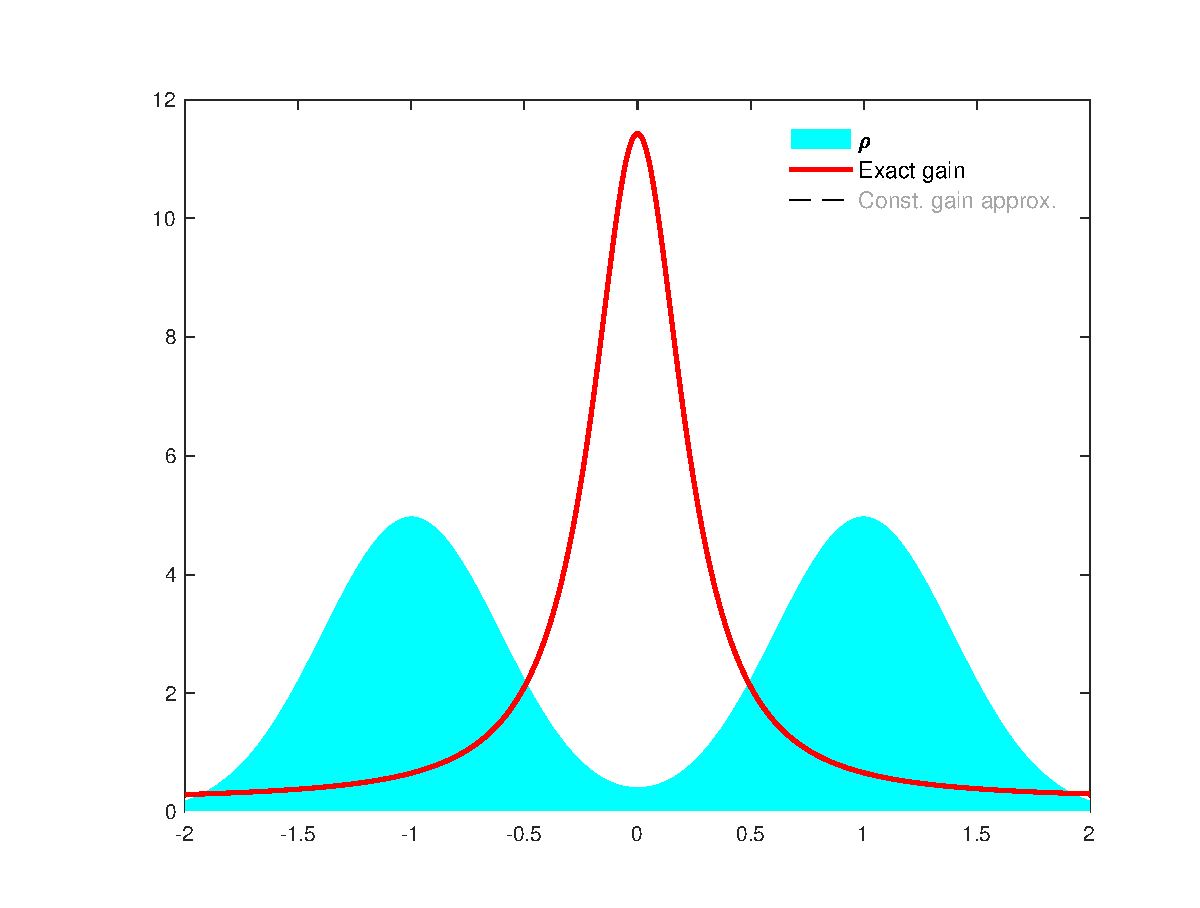
\includegraphics[width= .65\hsize]{gain_exact.eps}}
%		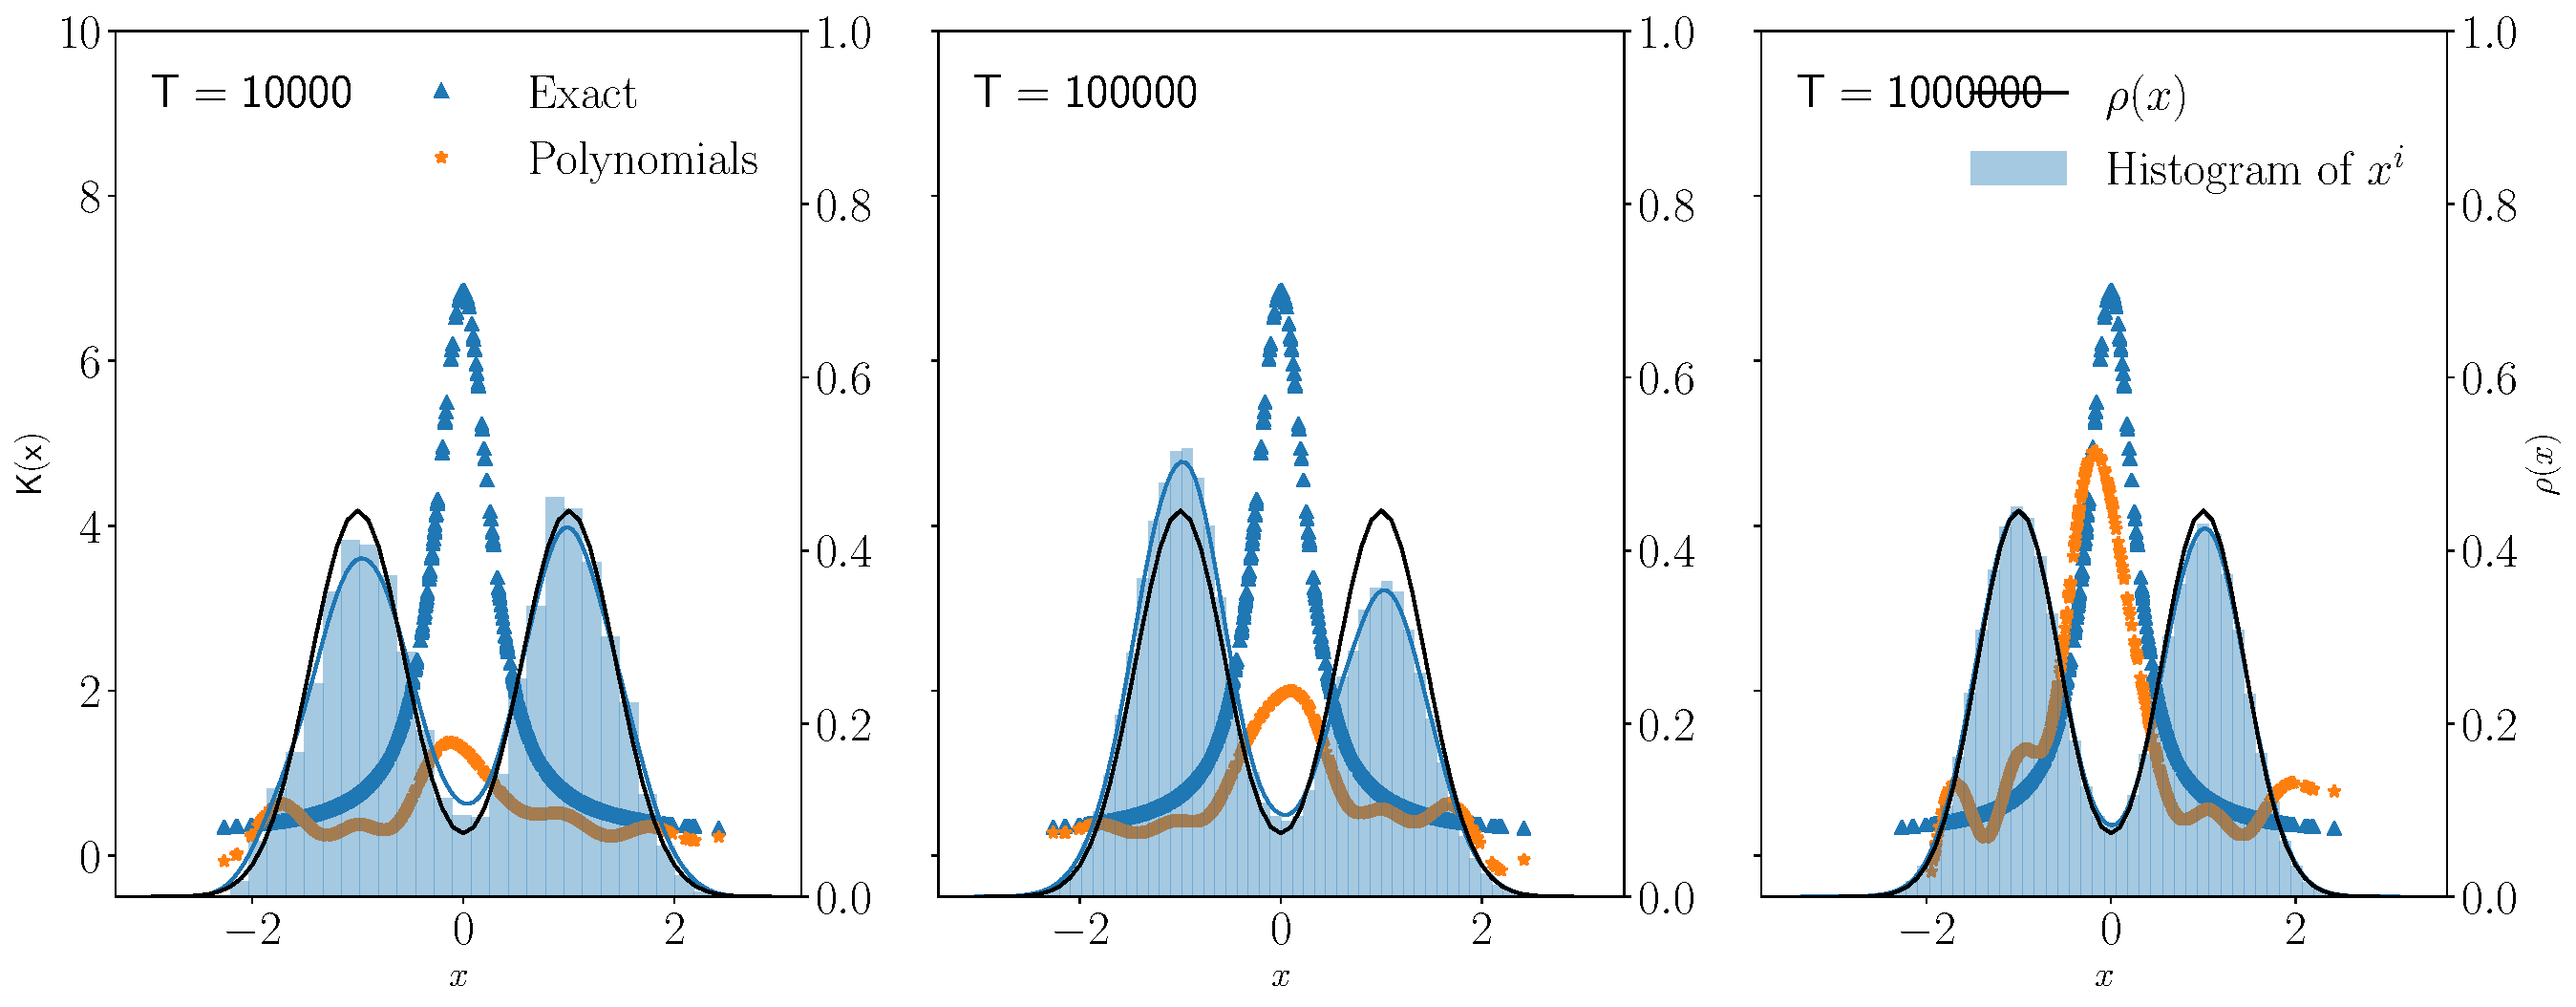
\includegraphics[width= \hsize]{Chap4_diff_td_linear_polynomials.pdf}\\
%	    $\gradTD$ with $\basis_i = x^i$ with $1 \leq i \leq 10$.}
%    
%	\only<3>{
%		\centering
%		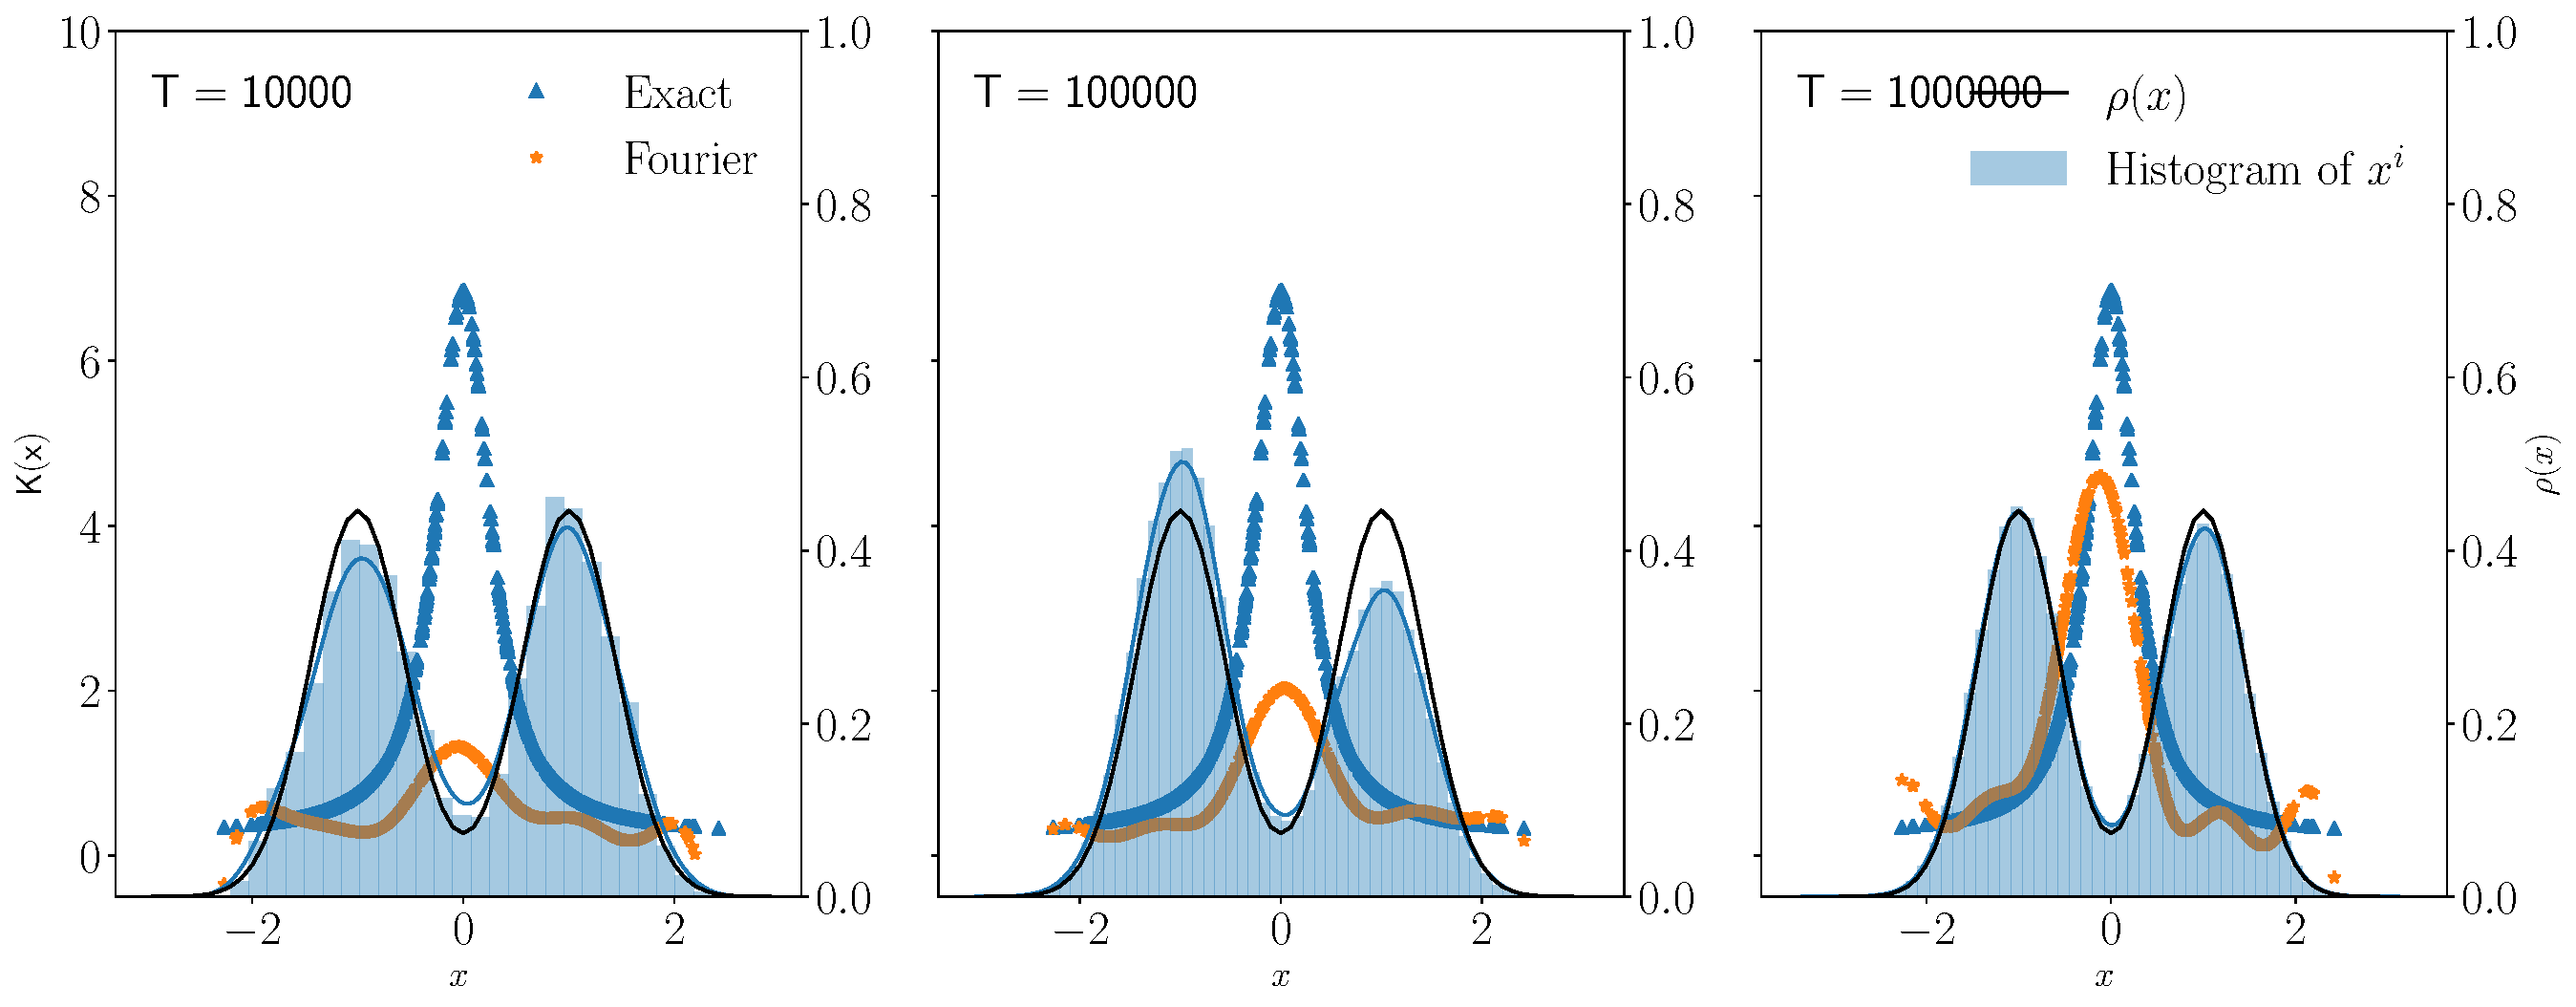
\includegraphics[width= \hsize]{Chap4_diff_td_linear_fourier.pdf}\\
%	  $\gradTD$ with $\basis_i = \sin ix, \, \basis_{i+1} = \cos ix$ with $1 \leq i \leq 5$.
%	}

	\only<2>{
		\centering
		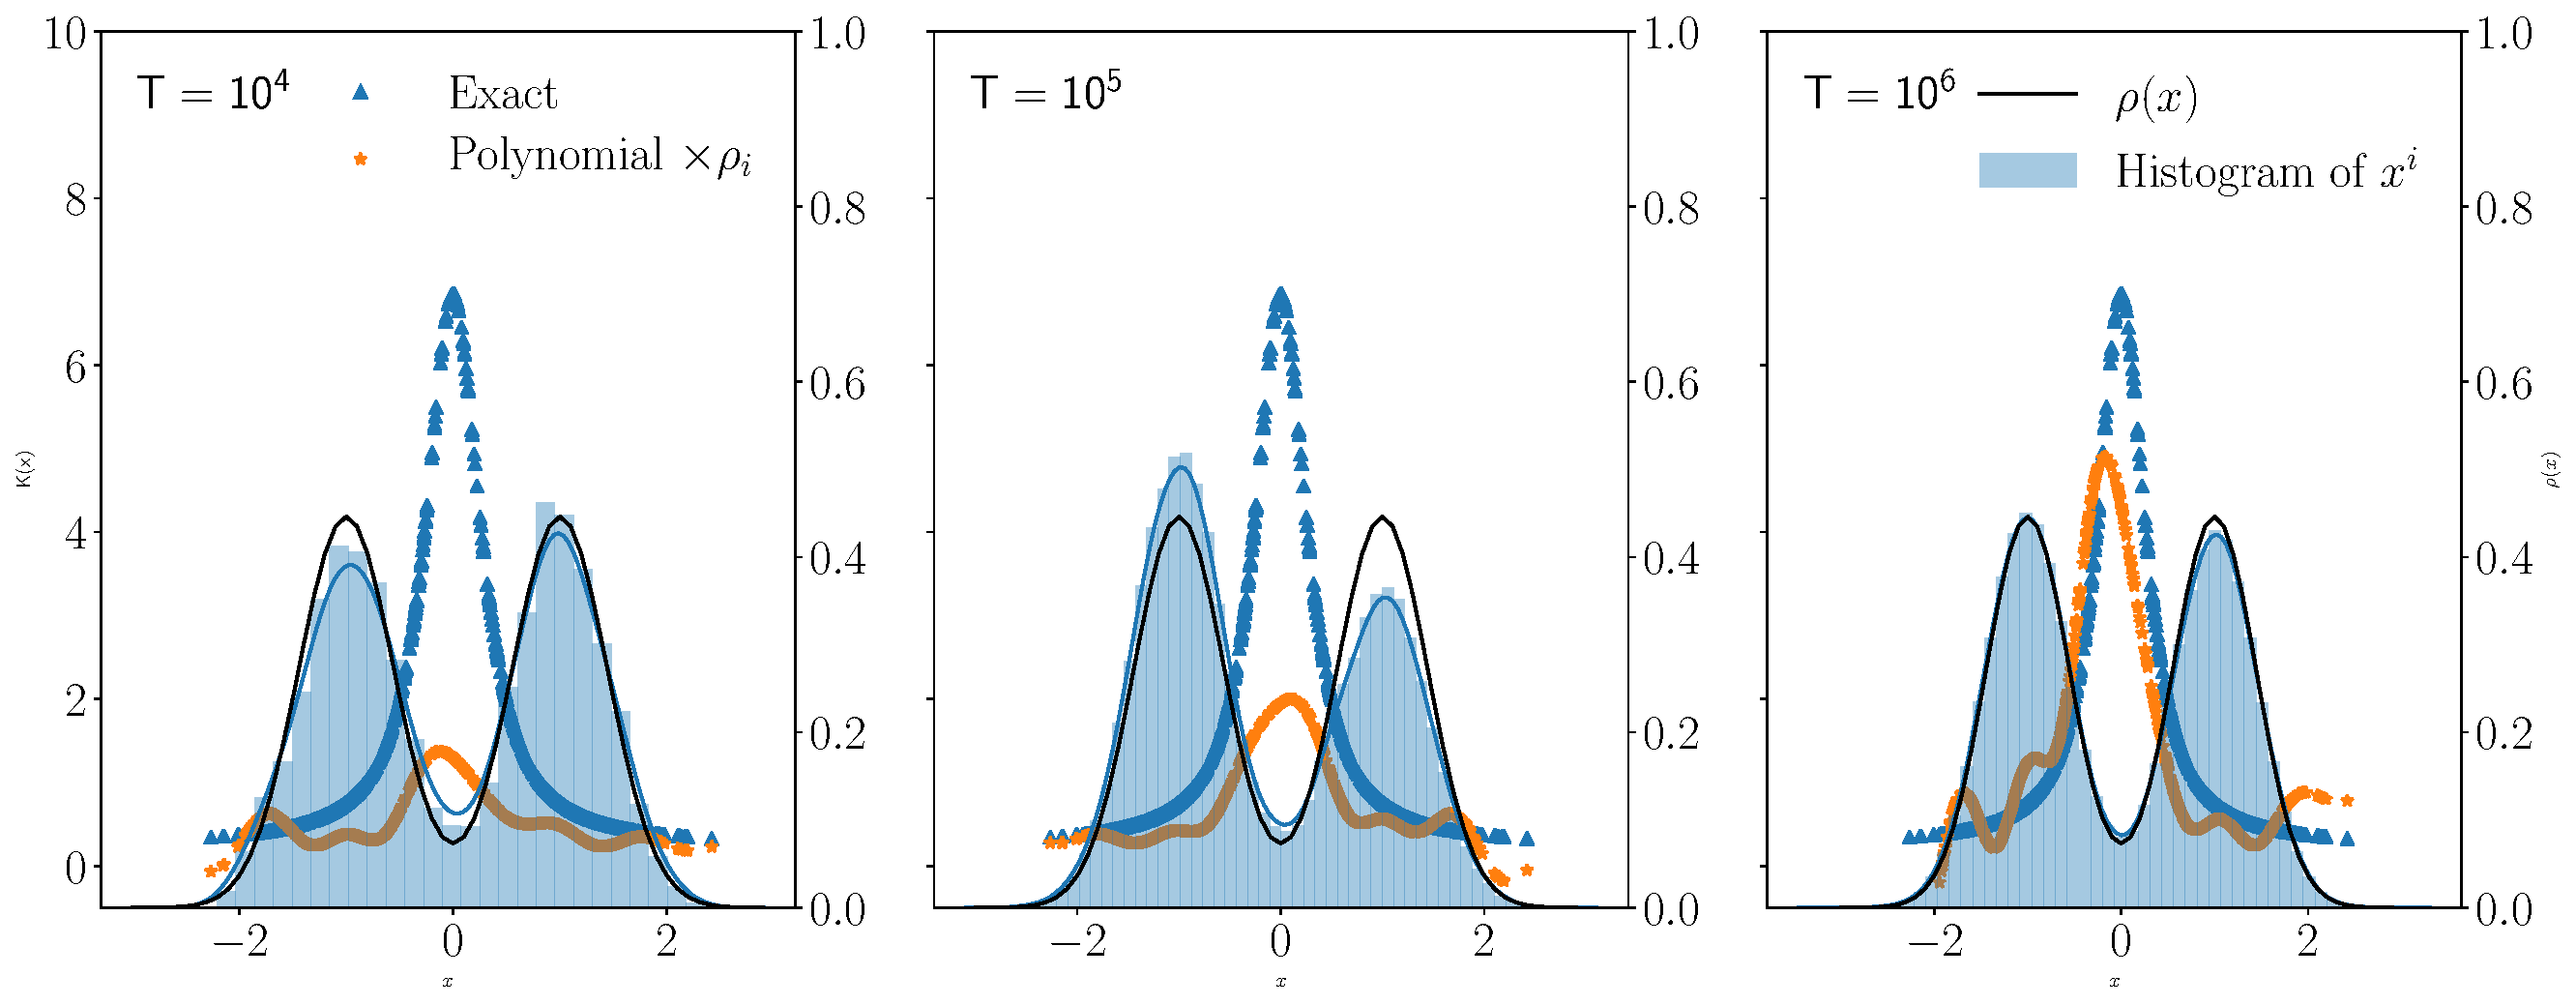
\includegraphics[width= \hsize]{Chap4_diff_td_linear_wt_polynomials.pdf}\\
	  $\gradTD$ with $\basis_i = x^i \pr_1(x), \, \basis_{i+1} = x^i \pr_2(x)$ with $1 \leq i \leq 5$.
	}
%	\only<5>{
%		\centering
%		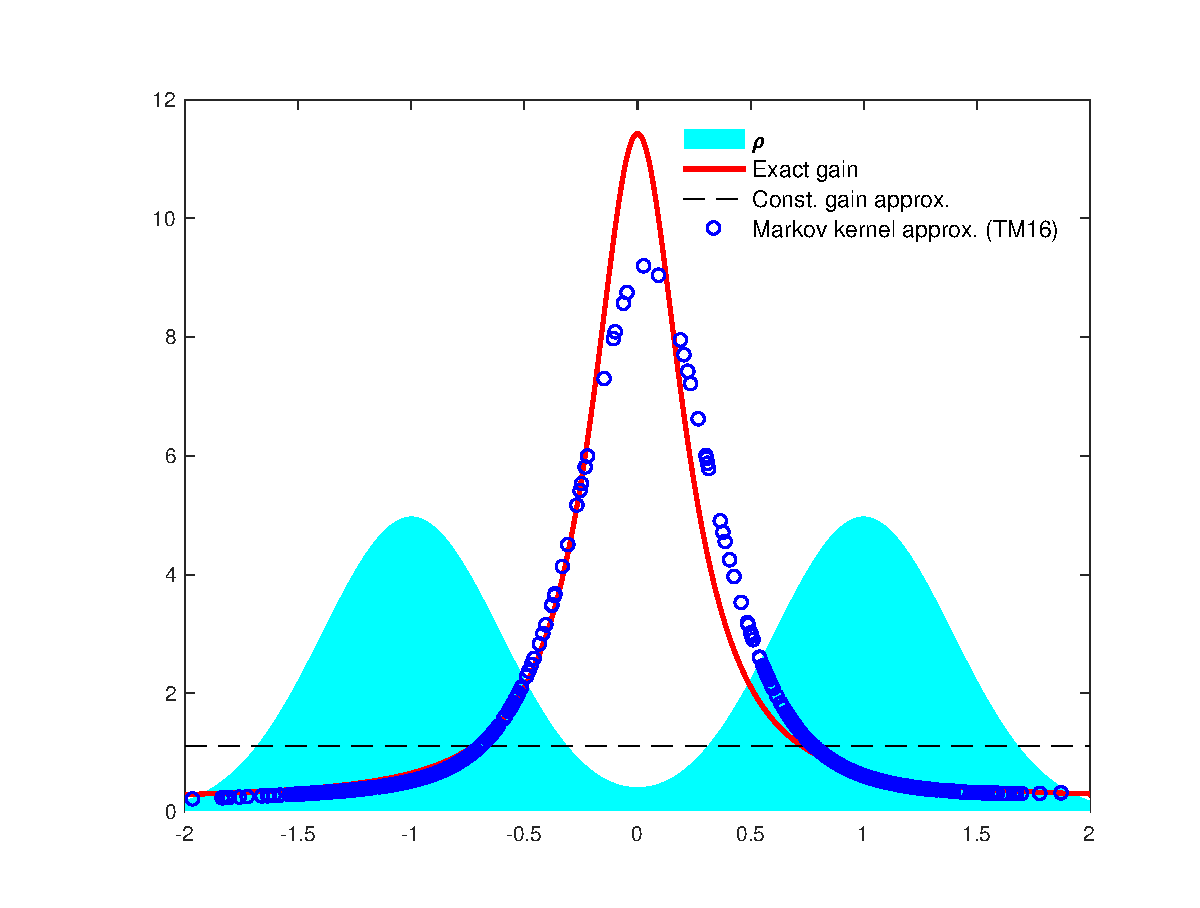
\includegraphics[width= .65\hsize]{gain_exact_const_coif.eps}}
%	
%	\only<6->{
%		\centering
%		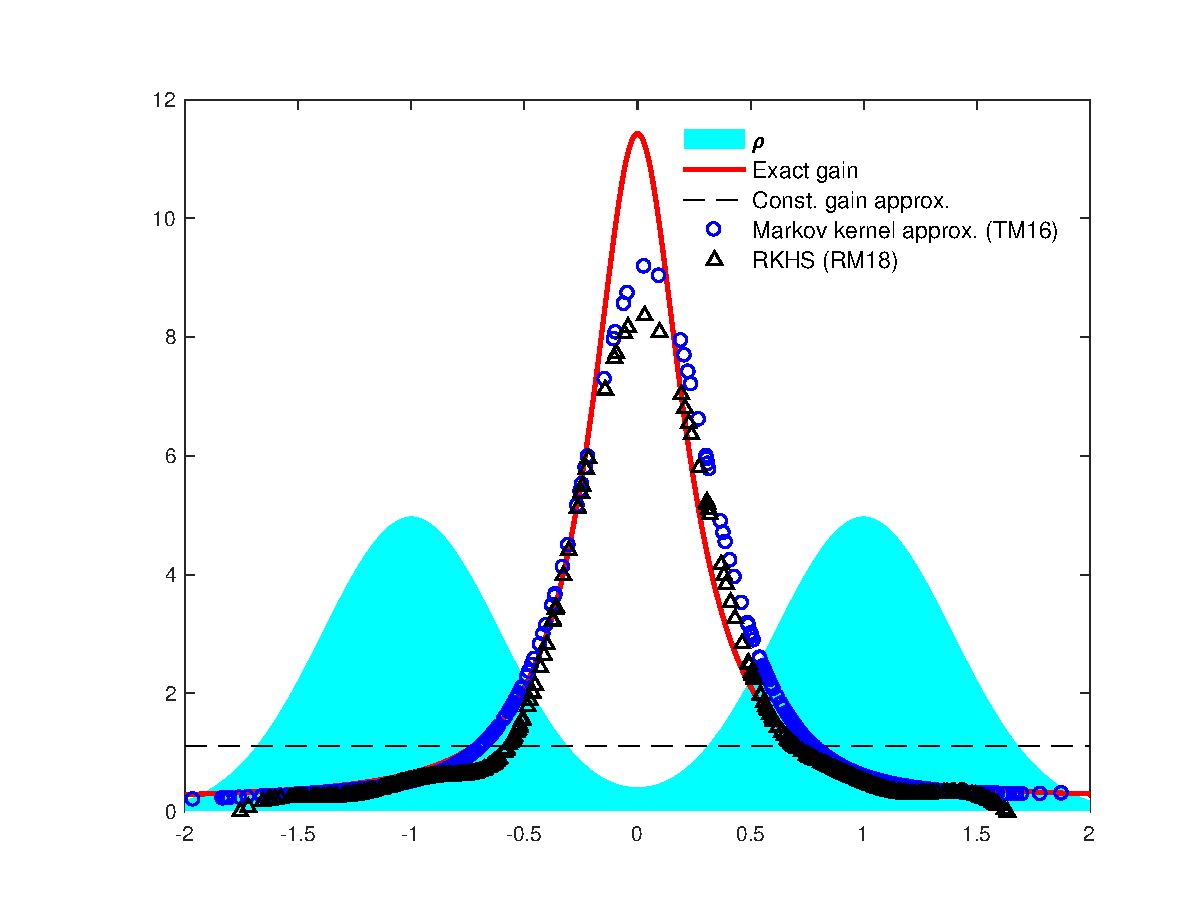
\includegraphics[width= .65\hsize]{gain_exact_const_coif_rkhs.eps}}
\end{minipage}
\end{frame}

\begin{frame}
\frametitle{Application to nonlinear filtering}
\framesubtitle{Numerical example - Gain approximation for a fixed $t$}
\begin{minipage}[t][6.5cm][t]{\textwidth}
	\begin{tabular}{lll}\alertb{Example:} &For a fixed $t$, $\pr_t$ a Gaussian mixture
		\\
		&   $c(x)\equiv x$
		\\
		& $N  = 100, 500, 1000$
	\end{tabular}

	\only<1>{
		\centering
		% 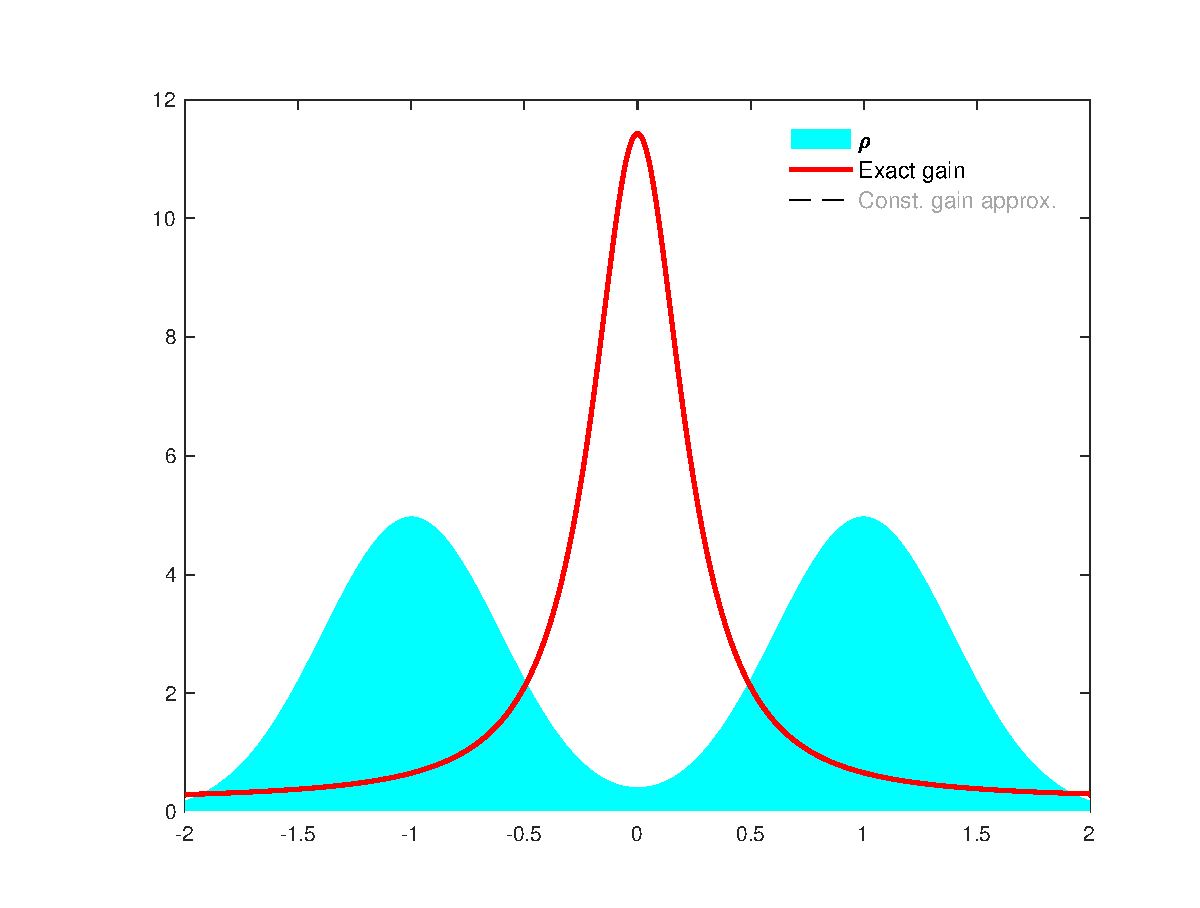
\includegraphics[width= .65\hsize]{gain_exact.eps}}
		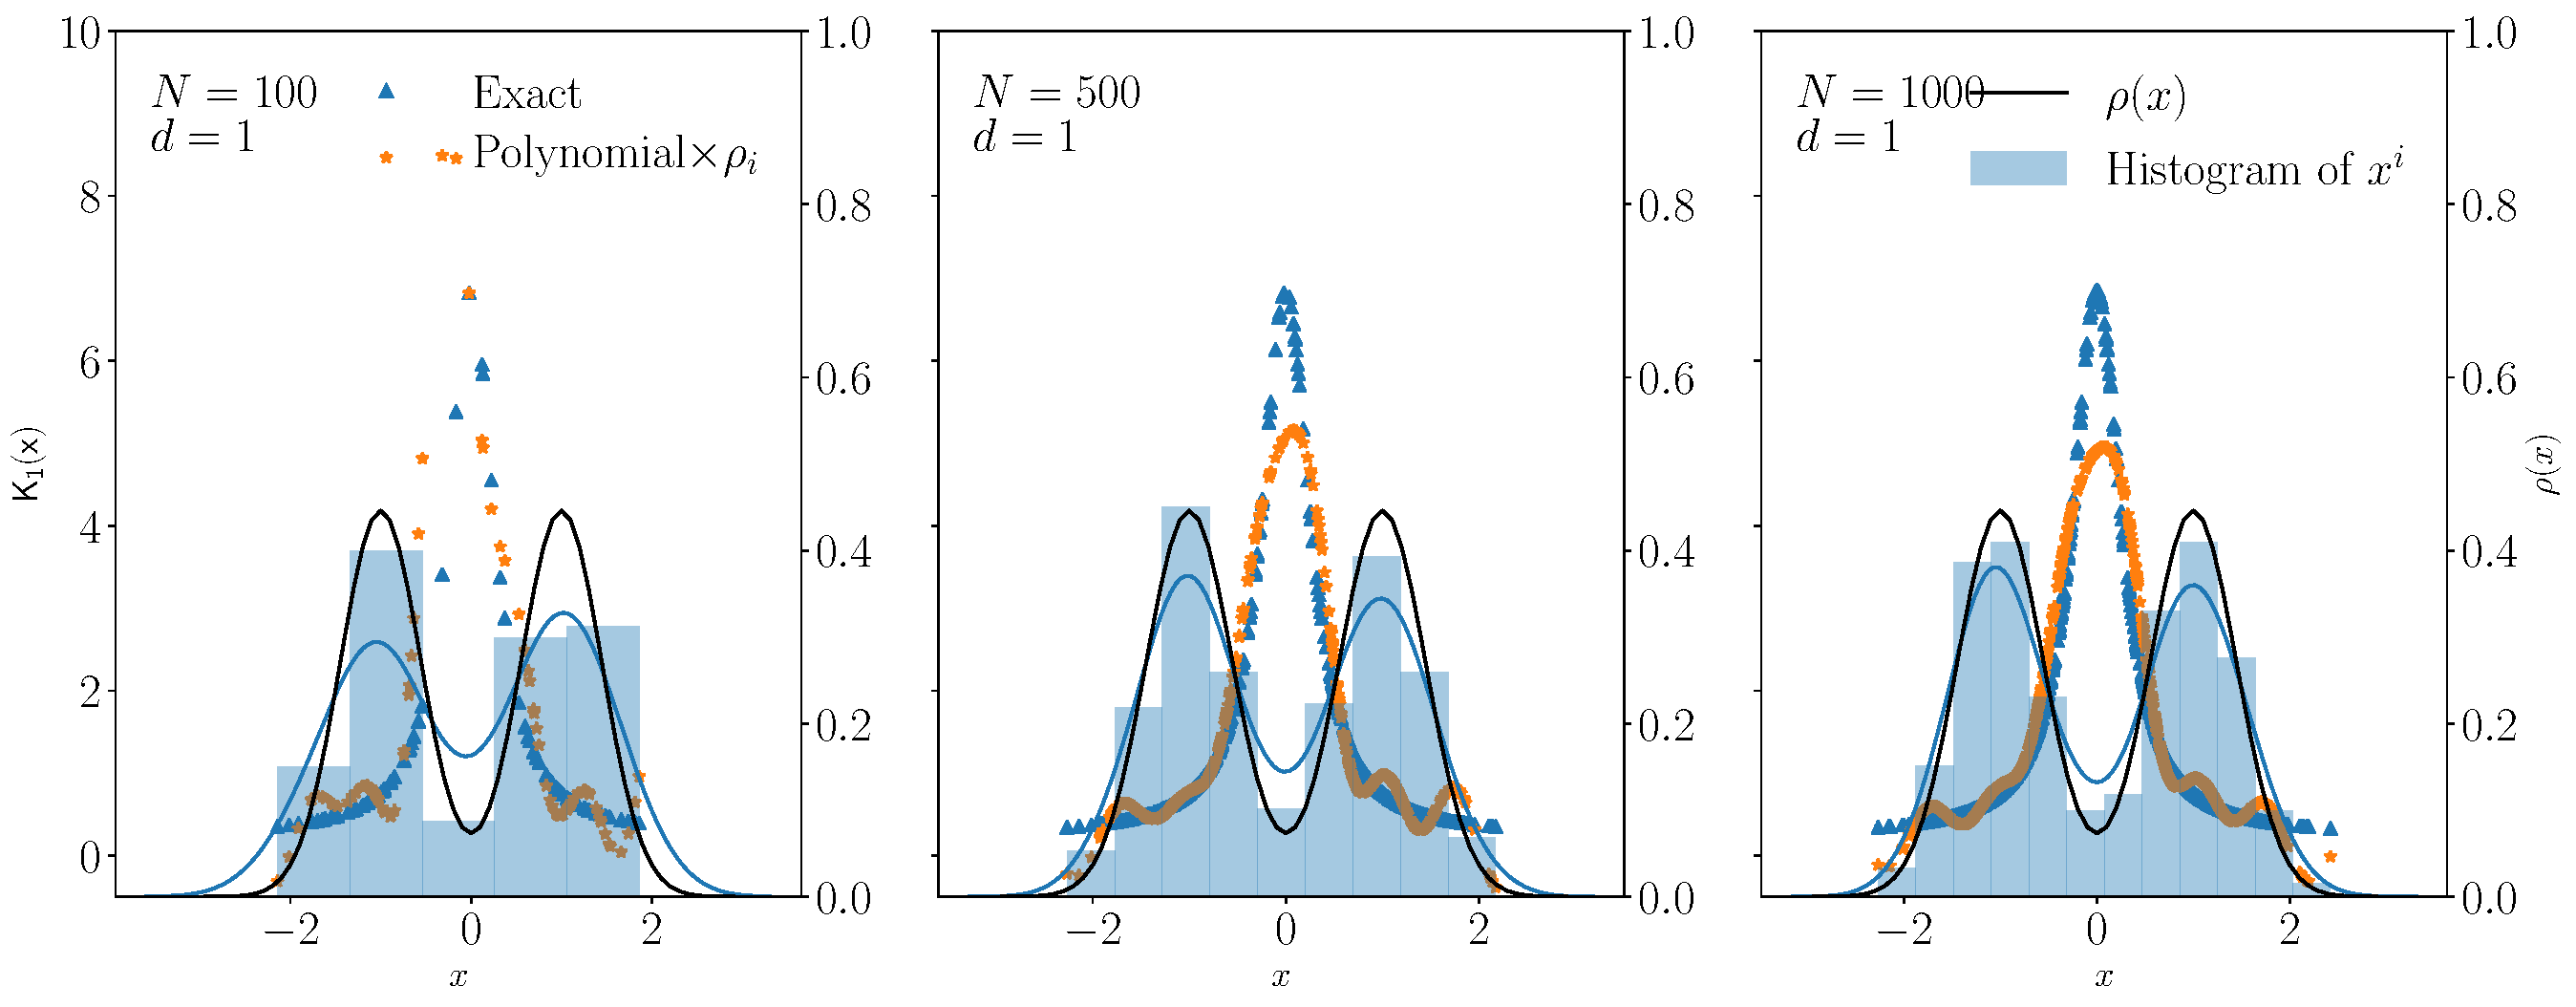
\includegraphics[width= \hsize]{Chap4_lang_td_wt_polynomials.pdf}\\
		$\gradTD$-L with $\basis_i = x^i \pr_1(x), \, \basis_{i+1} = x^i \pr_2(x)$ with $1 \leq i \leq 5$.
	}

	\only<2>{
	\centering 
	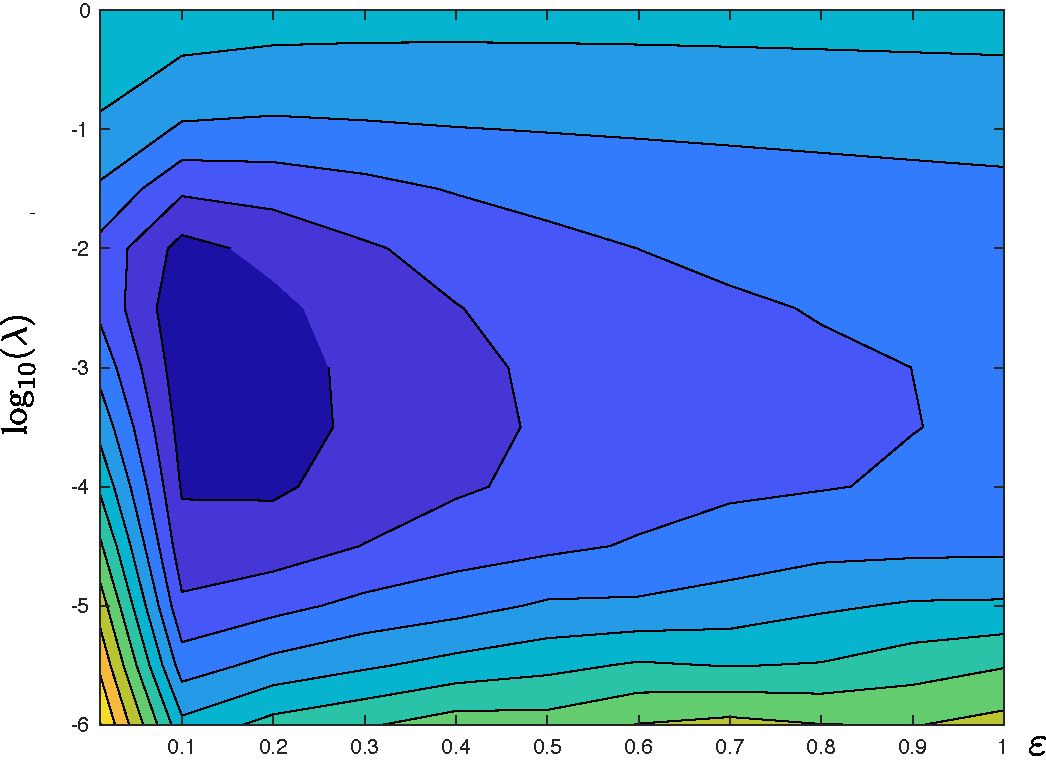
\includegraphics[width=0.5\hsize]{log_mse_contour_2m.pdf}\\
	Grid-search using $\Kern_\epsy \eqdef e^{-\frac{\|x-x'\|^2}{4 \epsy}}$, yields and $\epsy=0.1$ and $\lambda = 10^{-2}$ .
	}

	\only<3>{
	\centering
	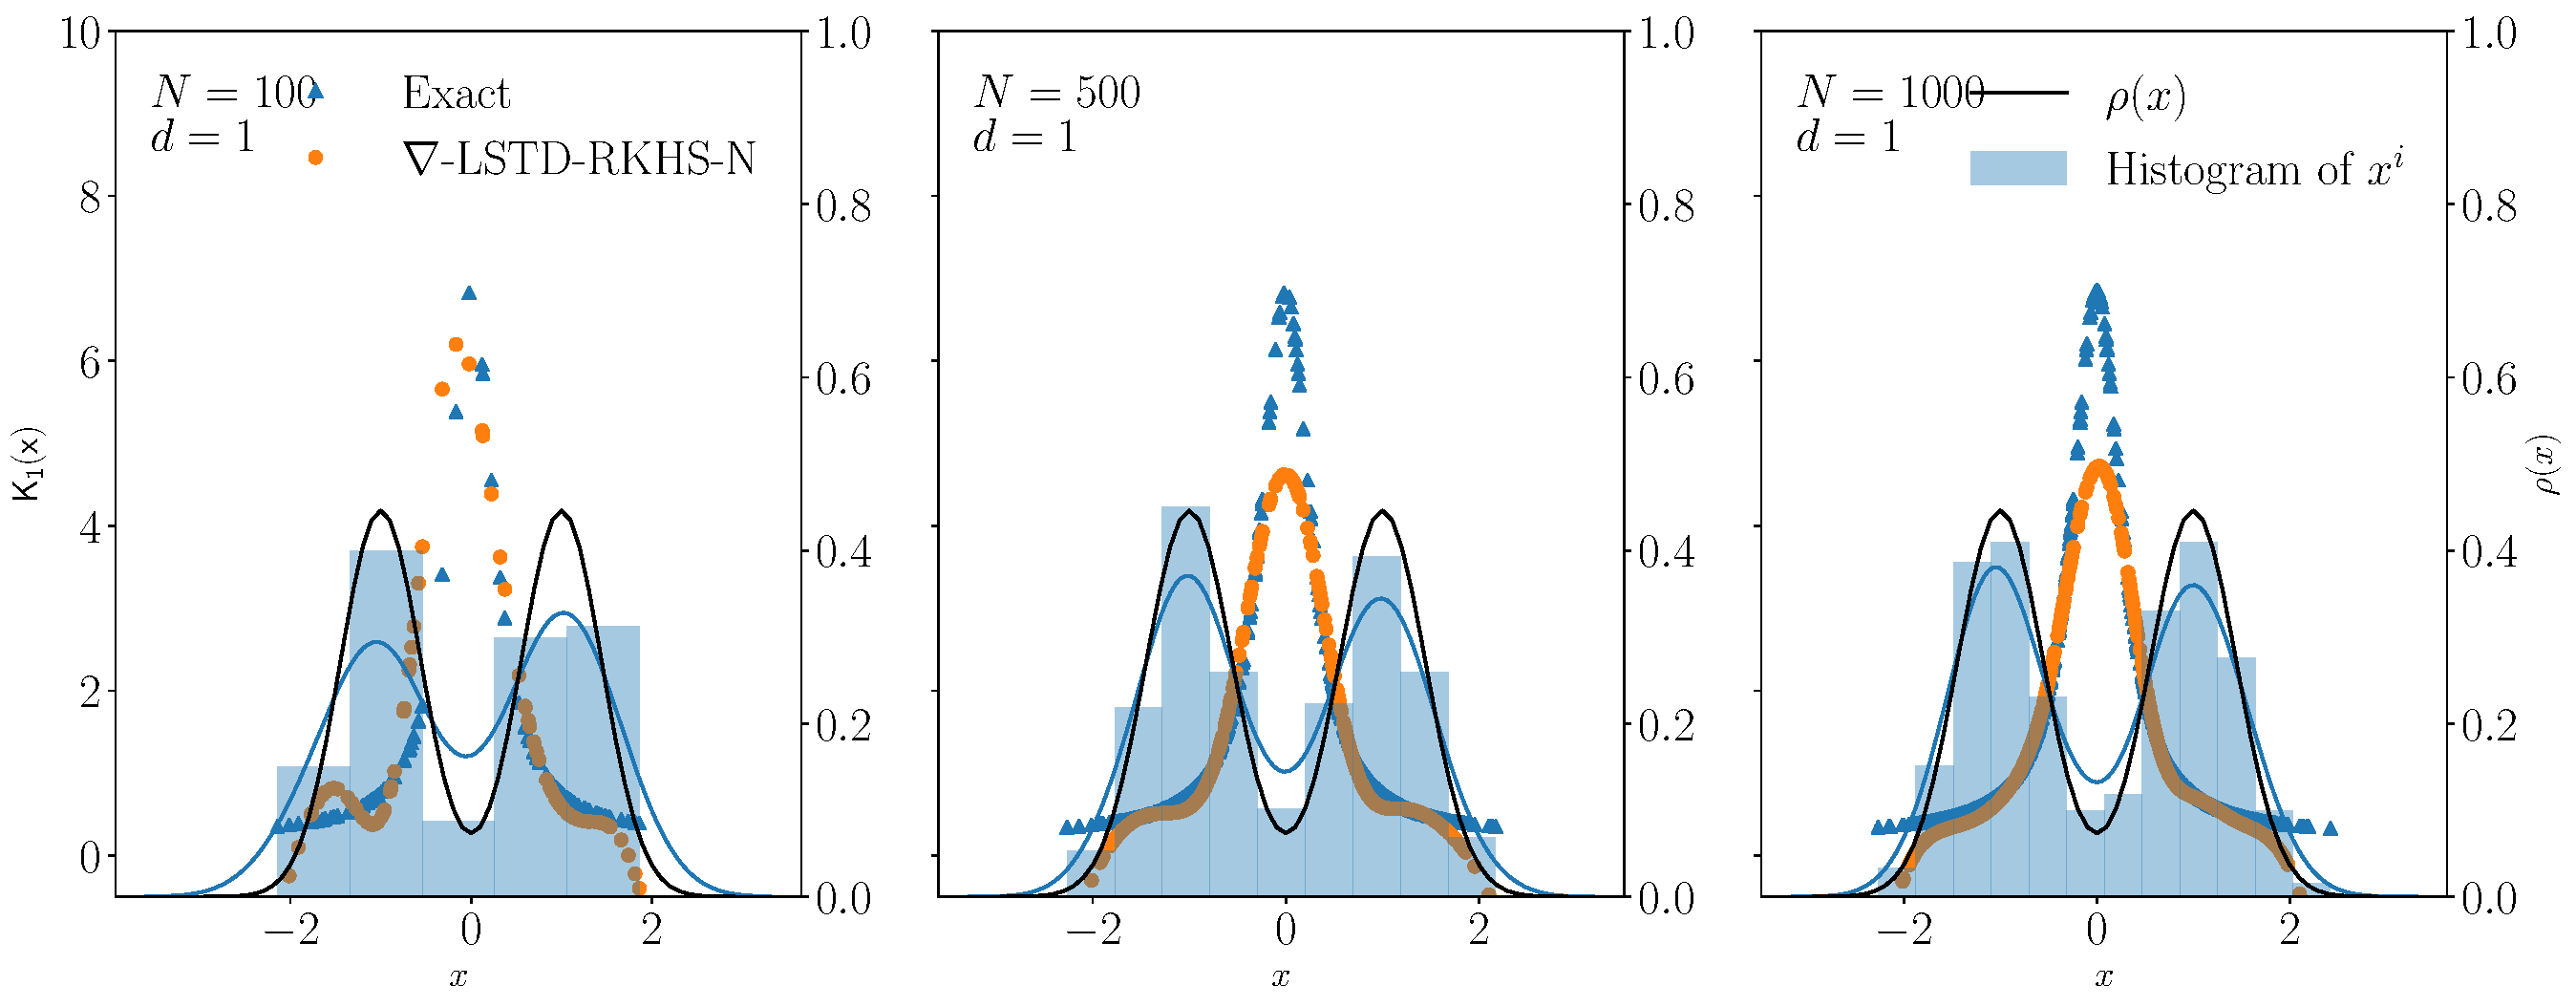
\includegraphics[width= \hsize]{Chap4_N.pdf}\\
	$\gradTD$-RKHS-N with Gaussian kernel, $\epsy=0.1$ and $\lambda = 10^{-2}$
    }

	\only<4>{
		\centering
		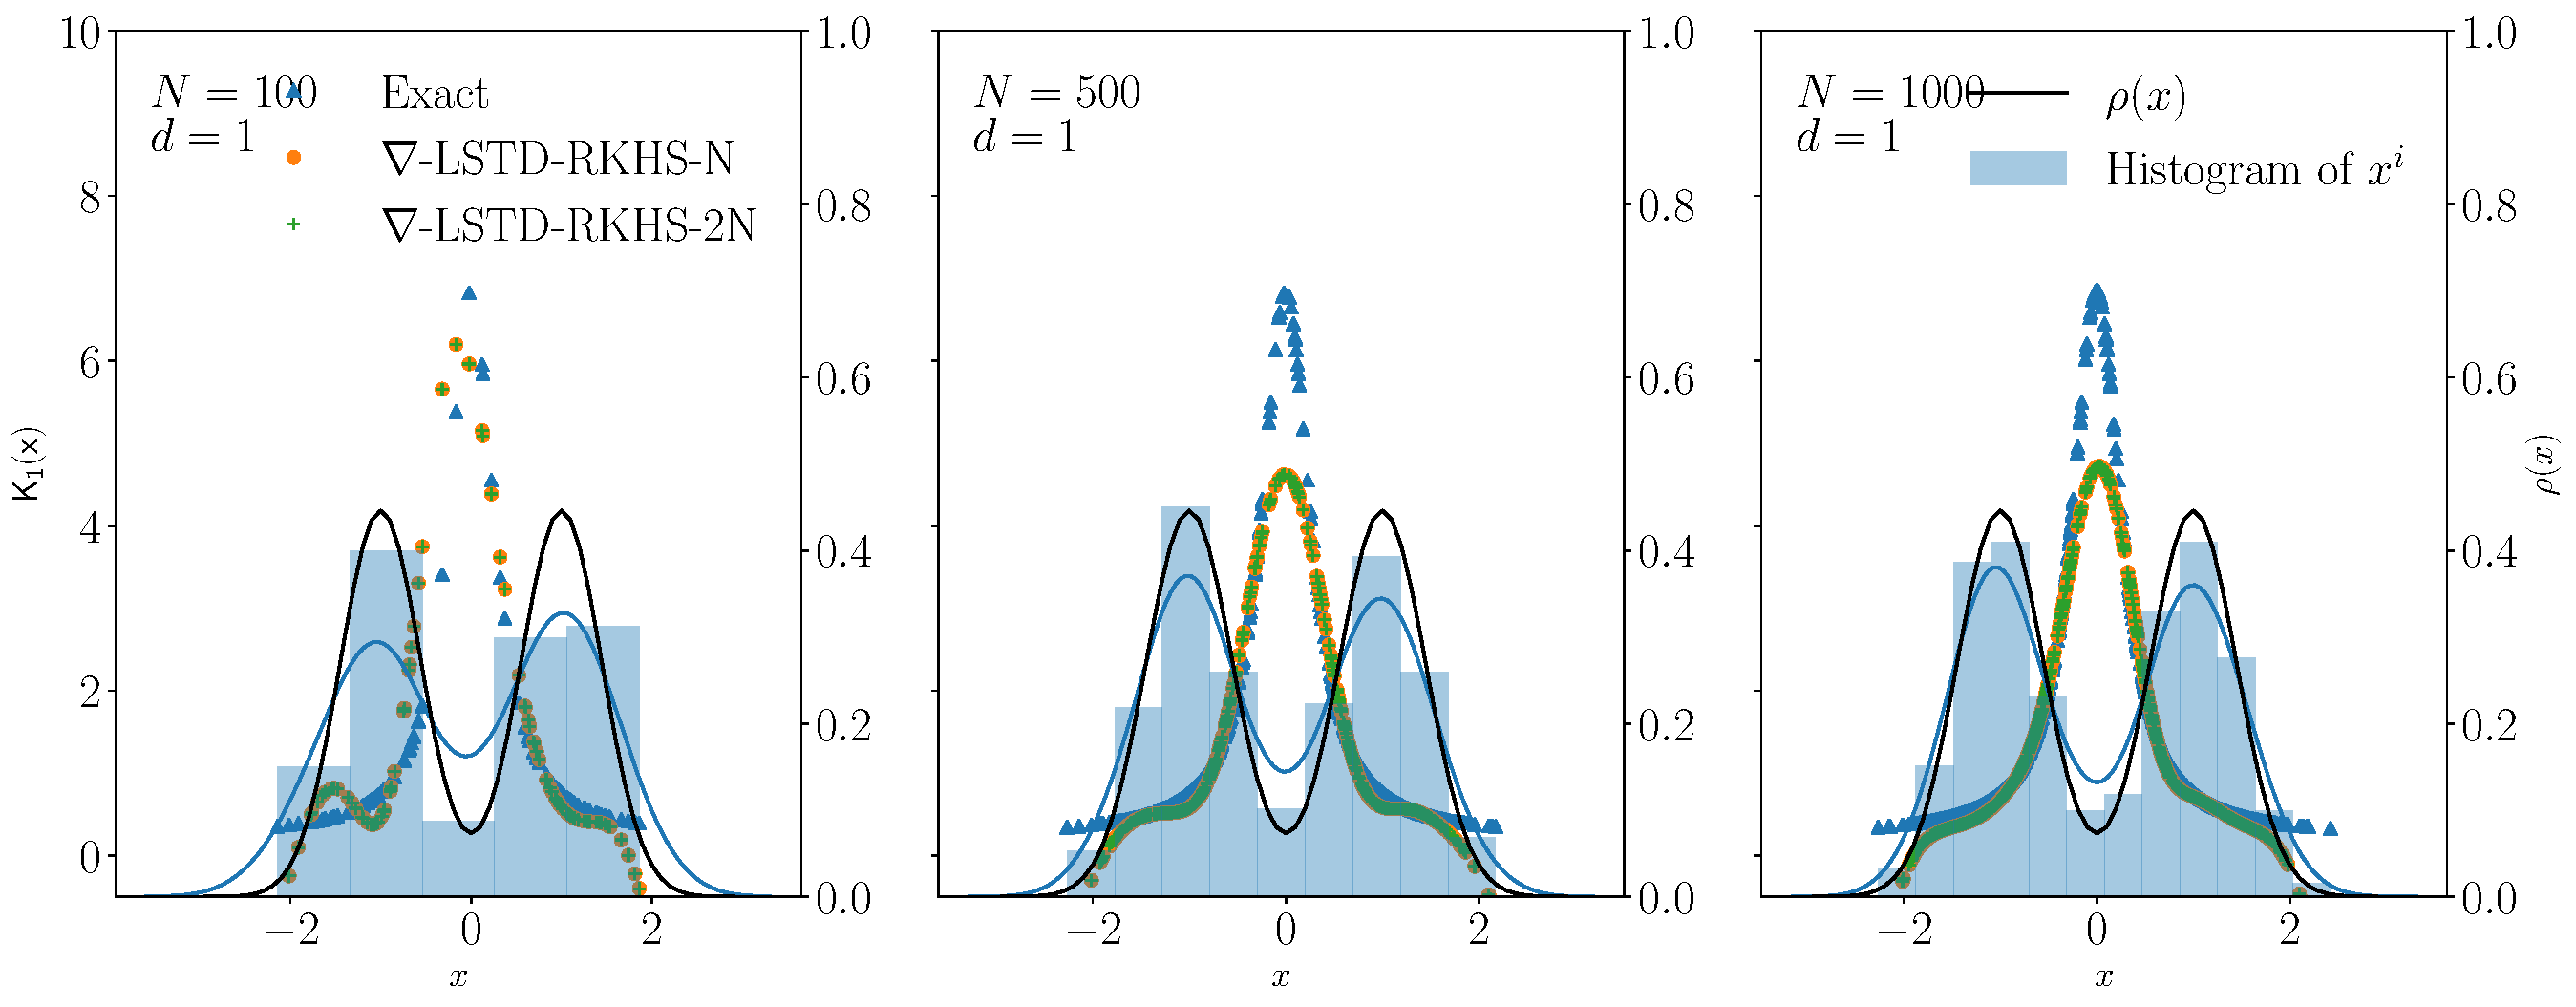
\includegraphics[width= \hsize]{Chap4_N_dN.pdf}\\
		$\gradTD$-RKHS-2N with Gaussian kernel, $\epsy=0.1$ and $\lambda = 10^{-2}$
	}

	\only<5>{
		\centering
		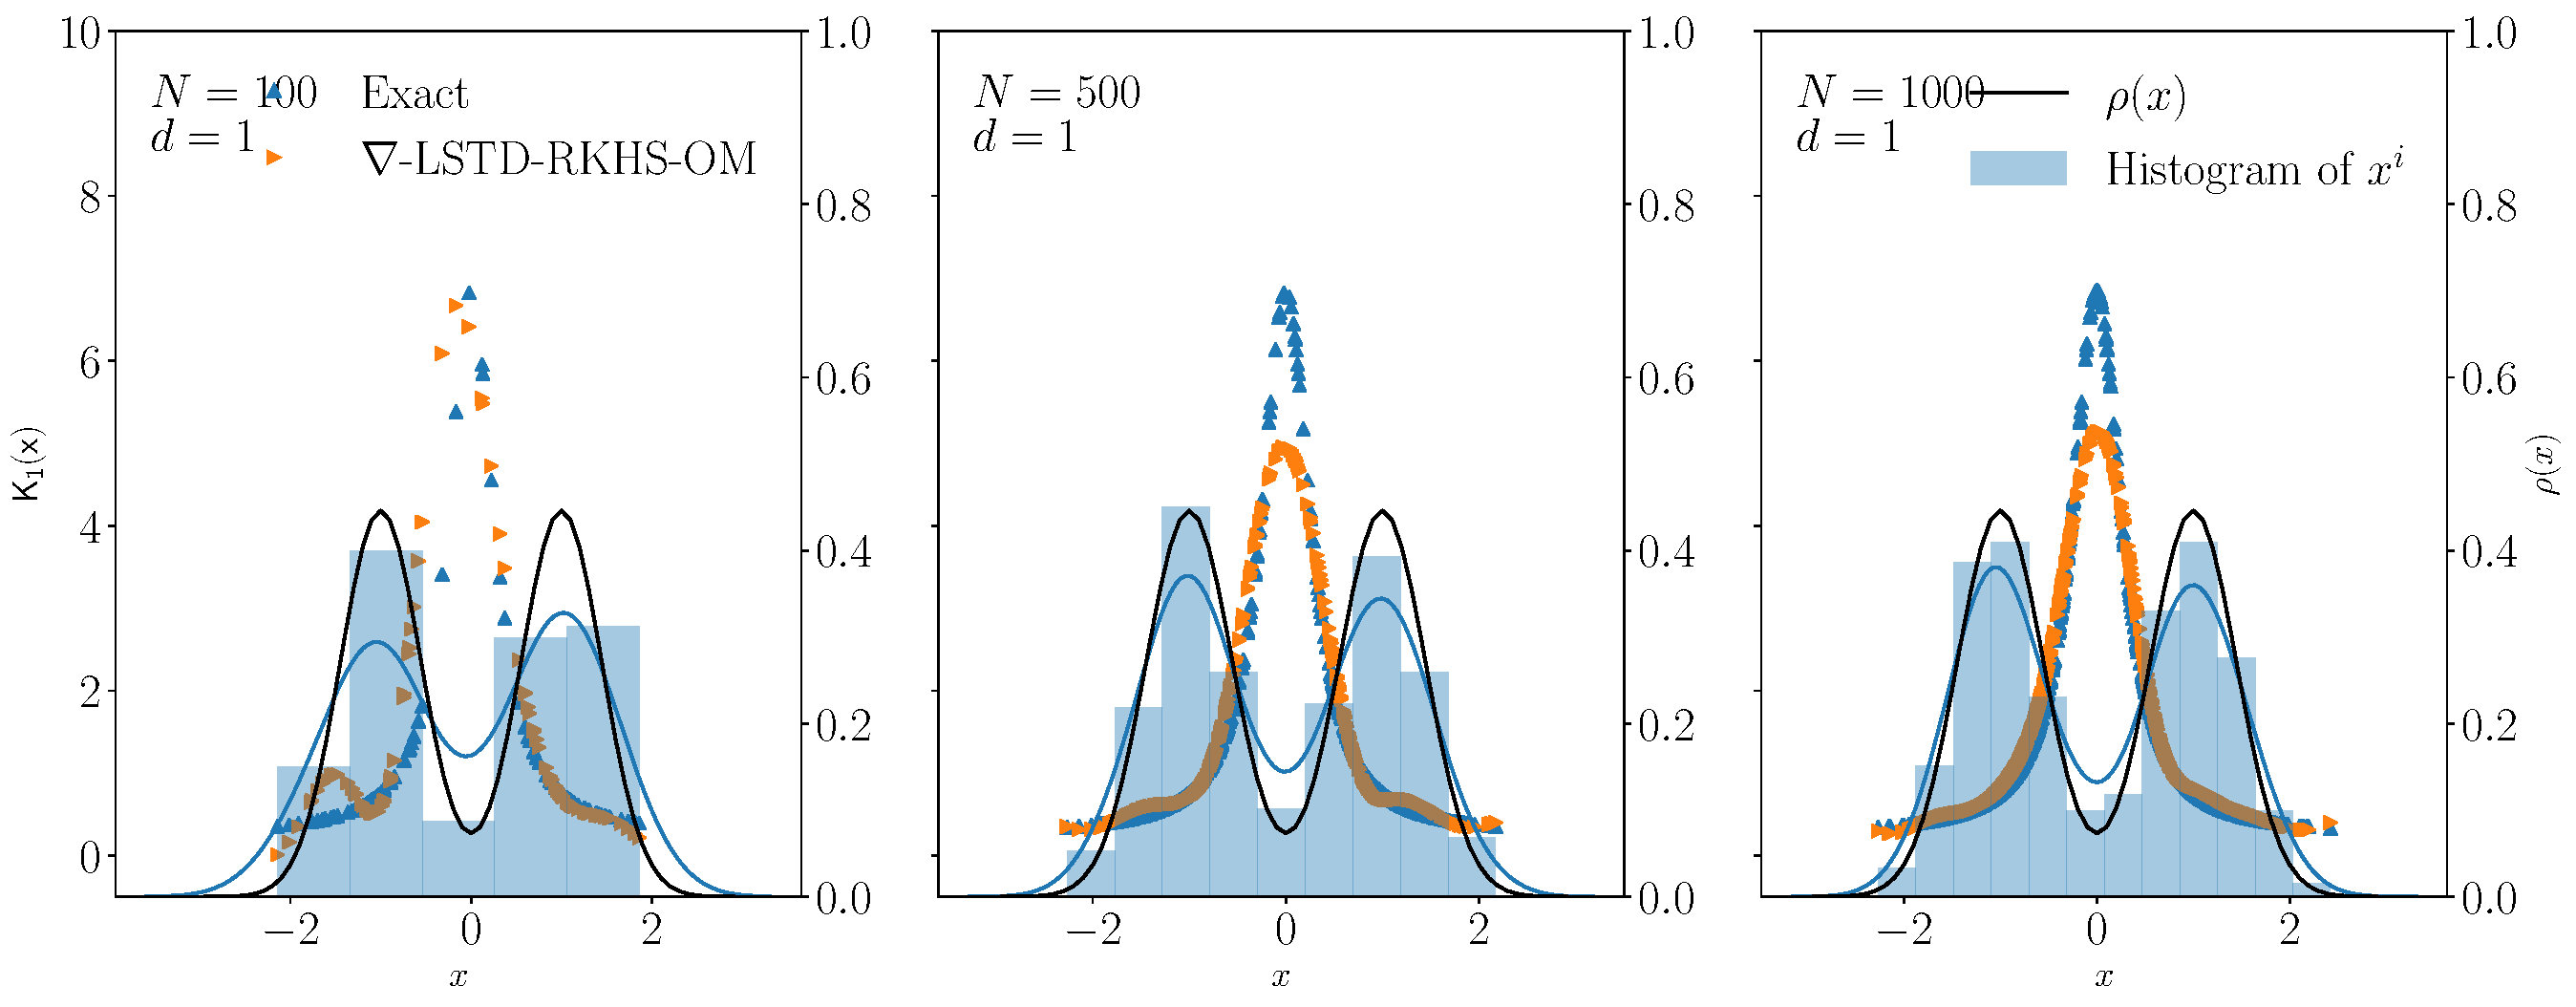
\includegraphics[width= \hsize]{Chap4_rkhs_om.pdf}\\
		$\gradTD$-RKHS-OM with Gaussian kernel, $\epsy=0.1$ and $\lambda = 10^{-2}$
	}

	\only<6>{
		\centering
		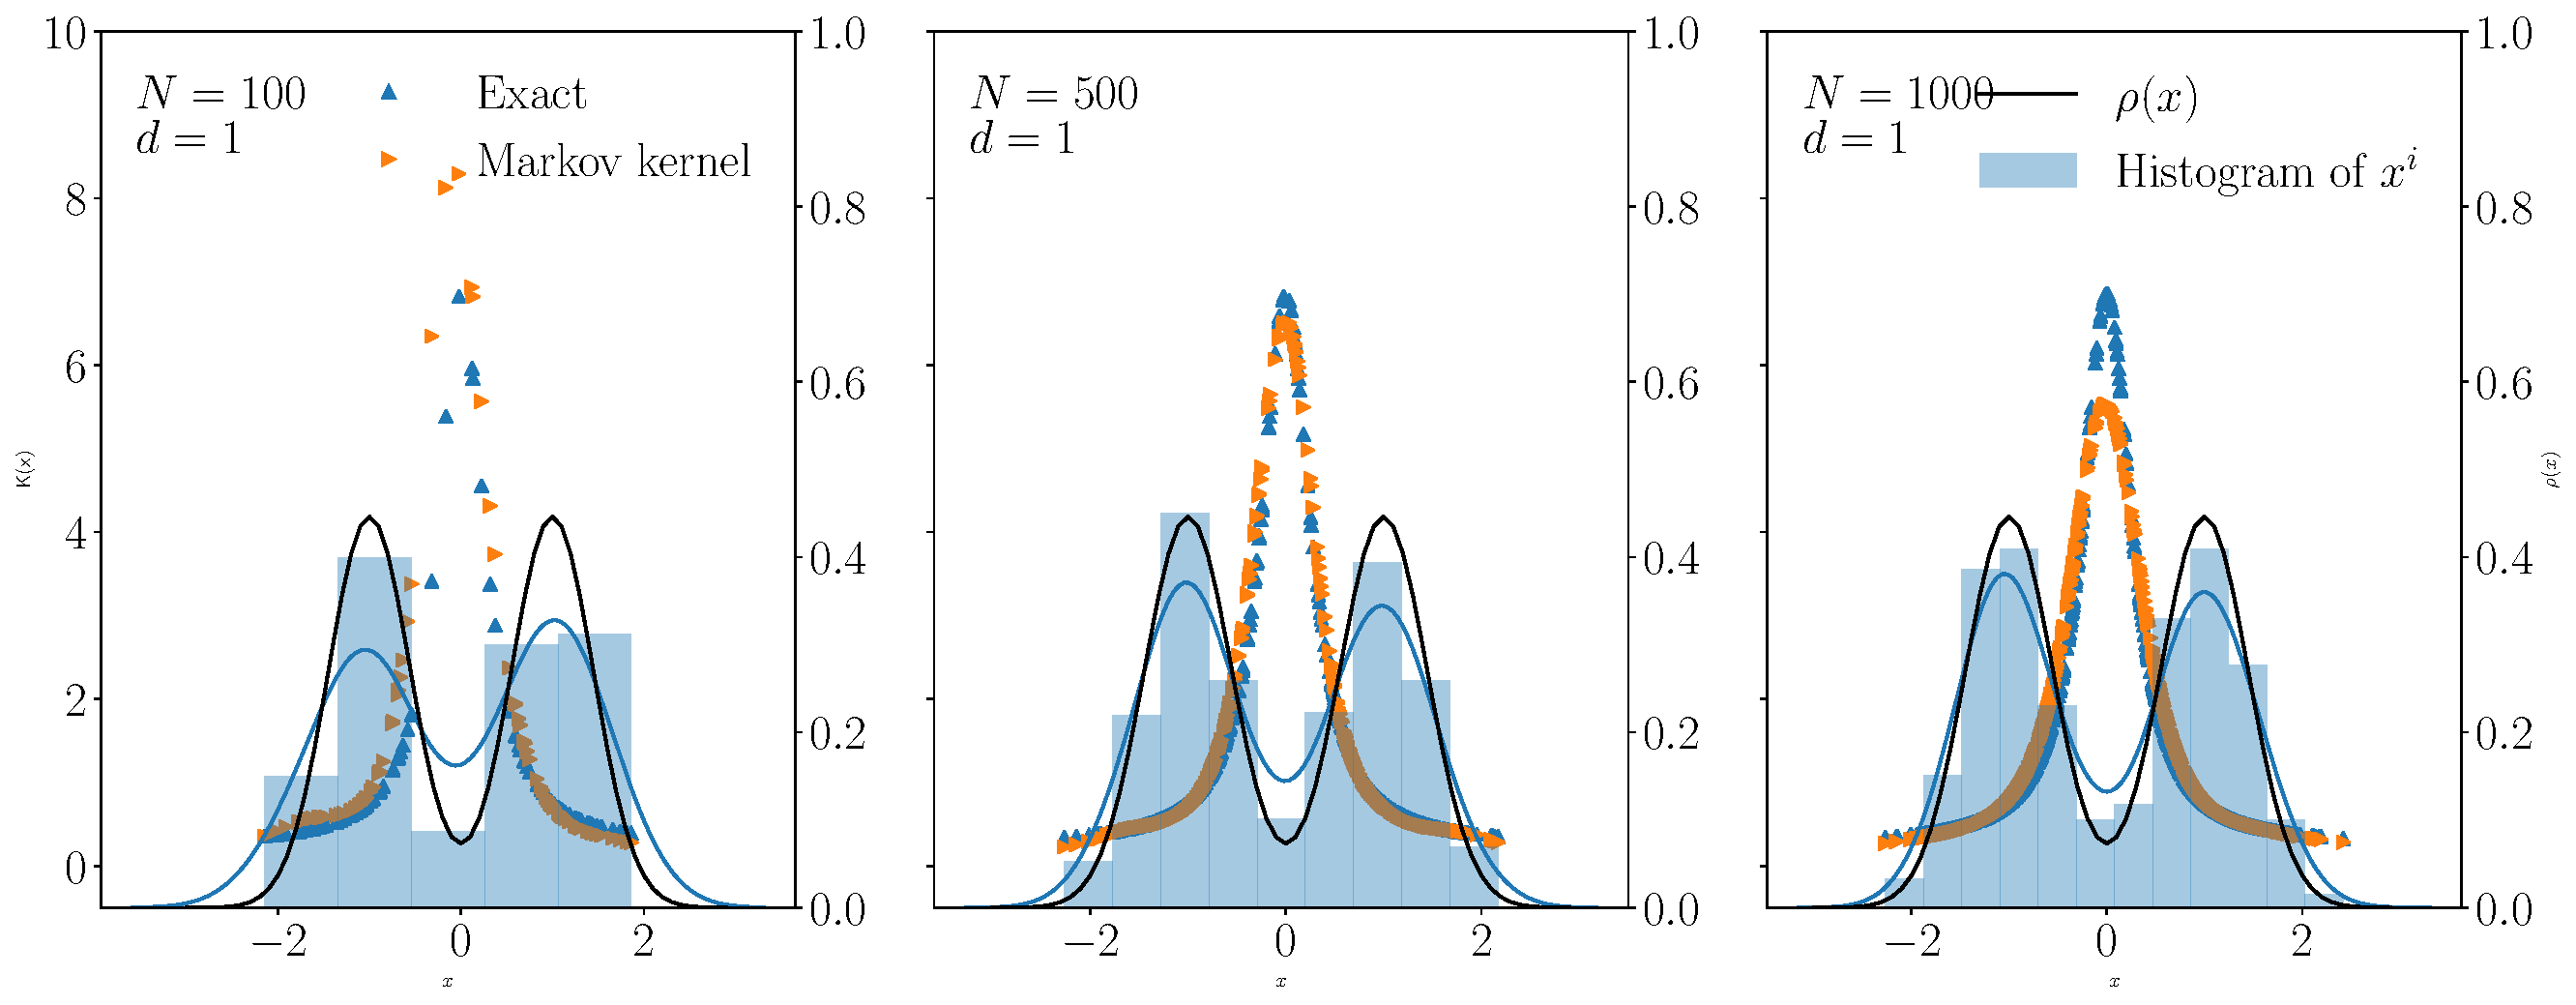
\includegraphics[width= \hsize]{Chap4_coif.pdf}\\
	 Markov kernel approximation with $\epsilon = 0.1$
	}

\only<7>{
	\centering
	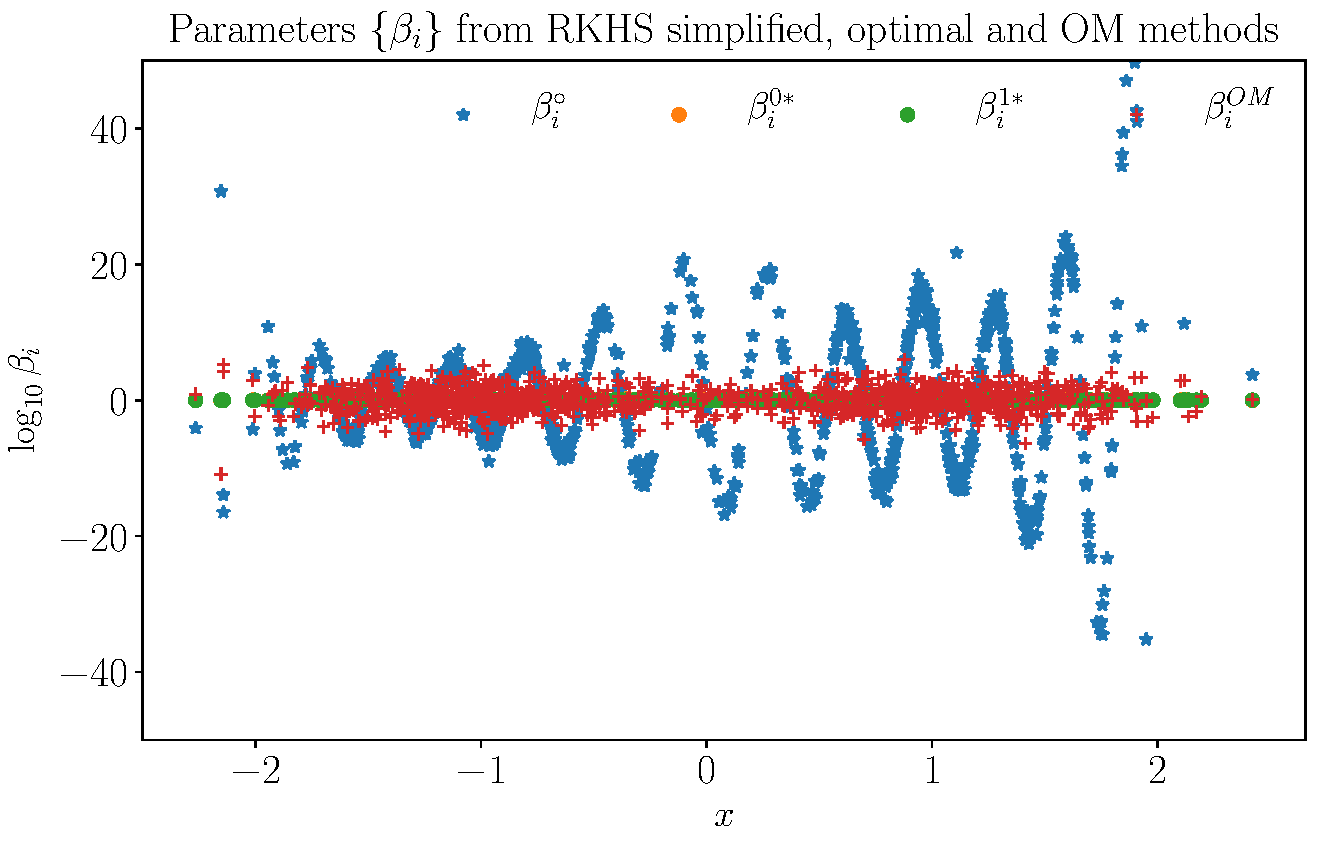
\includegraphics[width=0.75\hsize]{Chap4_beta_comparison.pdf}\\
	% Magnitudes of $\{\beta_i\}$ obtained from $\gradTD$-RKHS-2N, $\gradTD$-RKHS-N and $\gradTD$-RKHS-OM algorithms
}

\only<8>{
	\centering
	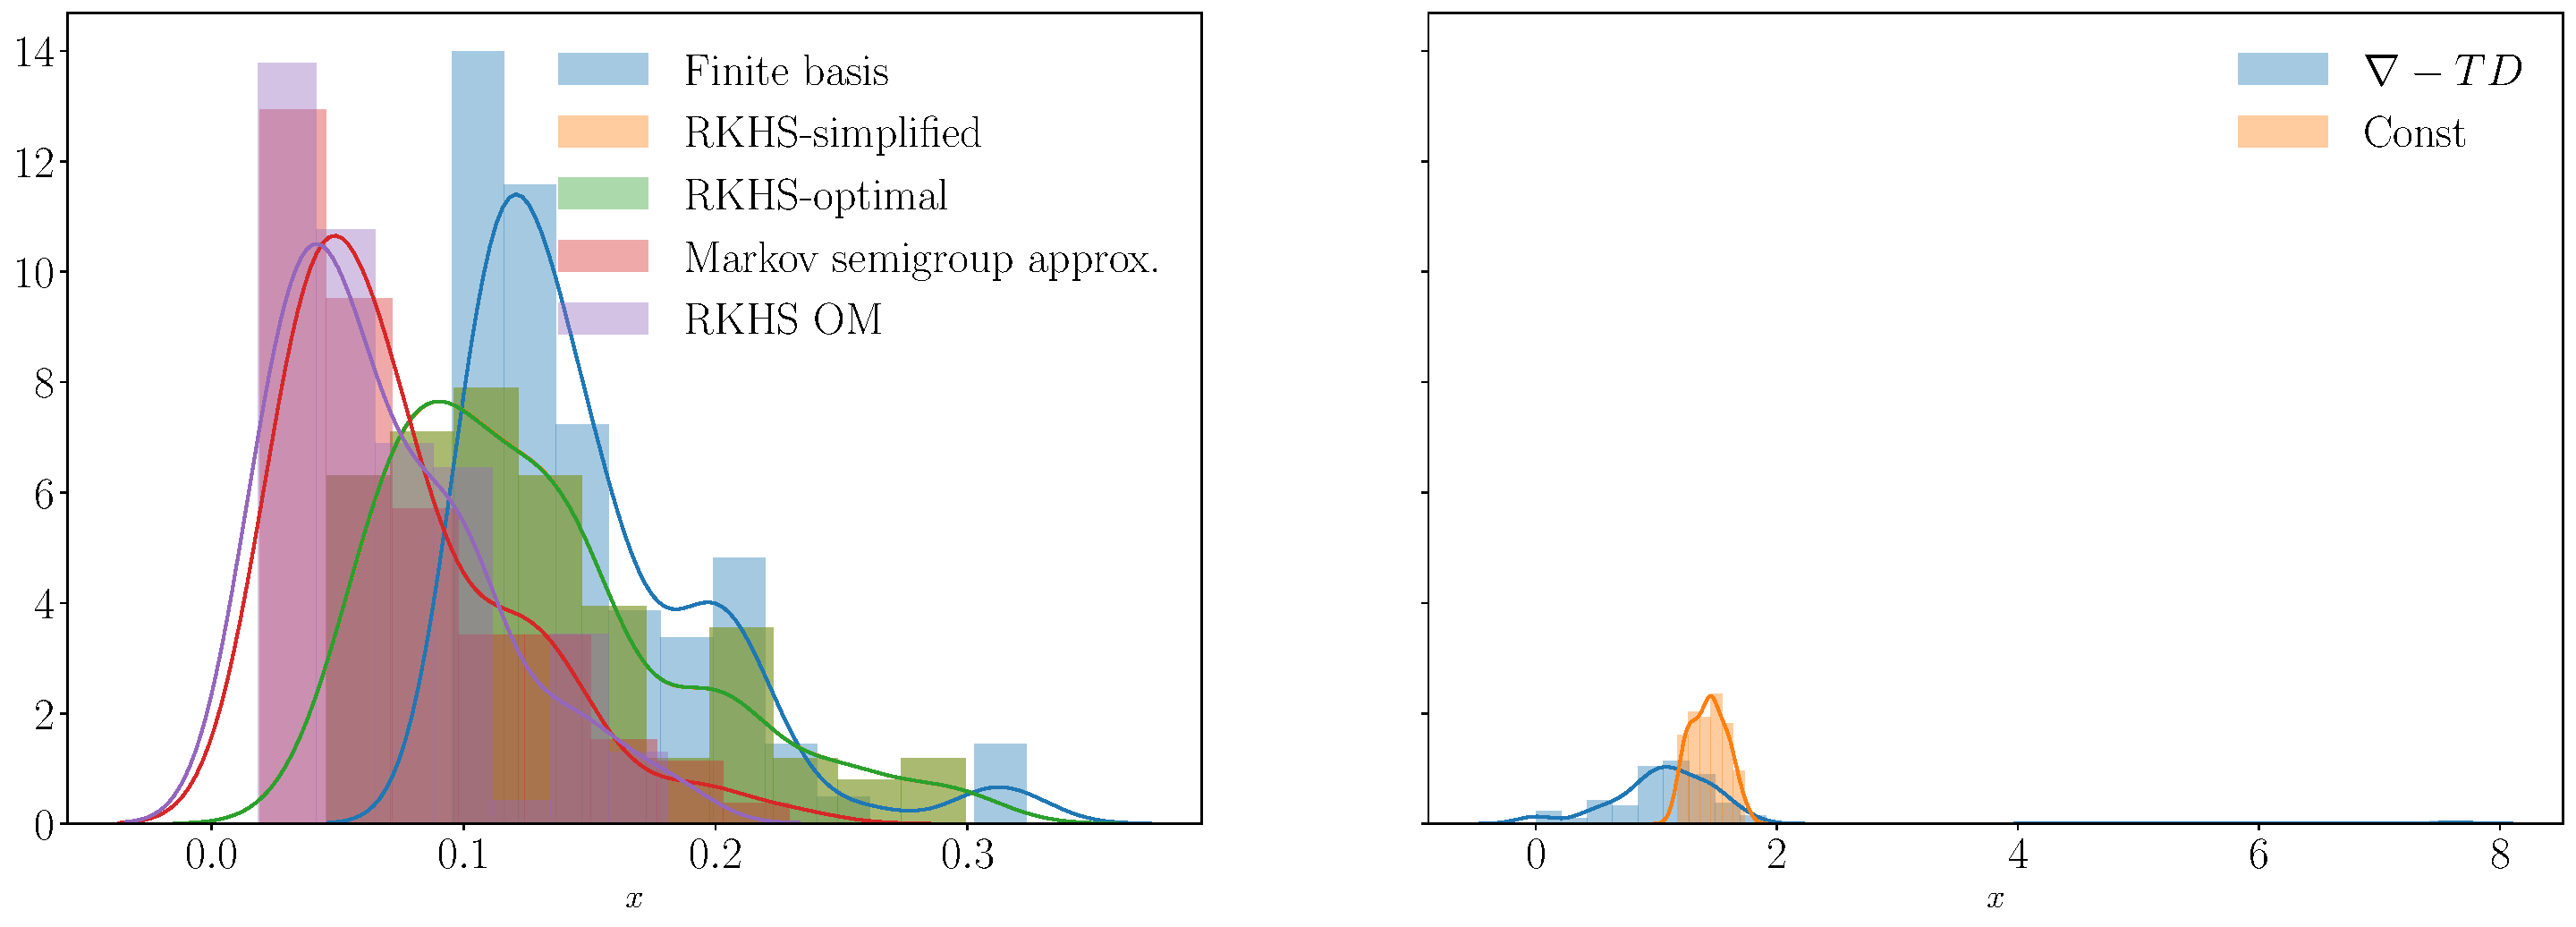
\includegraphics[width= \hsize]{Chap4_hist_mse_d1_runs100.pdf}\\
	Histogram of MSEs obtained from $100$ independent trials
}
\end{minipage}
\end{frame}

\begin{frame}
\frametitle{Application to nonlinear filtering}
\framesubtitle{Numerical example - Gain approximation for a fixed $t$}
\begin{minipage}[t][6.5cm][t]{\textwidth}
	\begin{tabular}{lll}\alertb{Example:} & $\pr(x) = \prod_{k=1}^d \pr_k(x_k)$
		\\
		&   $c(x) = C^\transpose x$, where $ C = \ind_d$
		\\
		& $d  = 2,5,10, \quad N = 1000$
		% \\
	\end{tabular}
%
%	\only<1>{
%		\centering
%		% 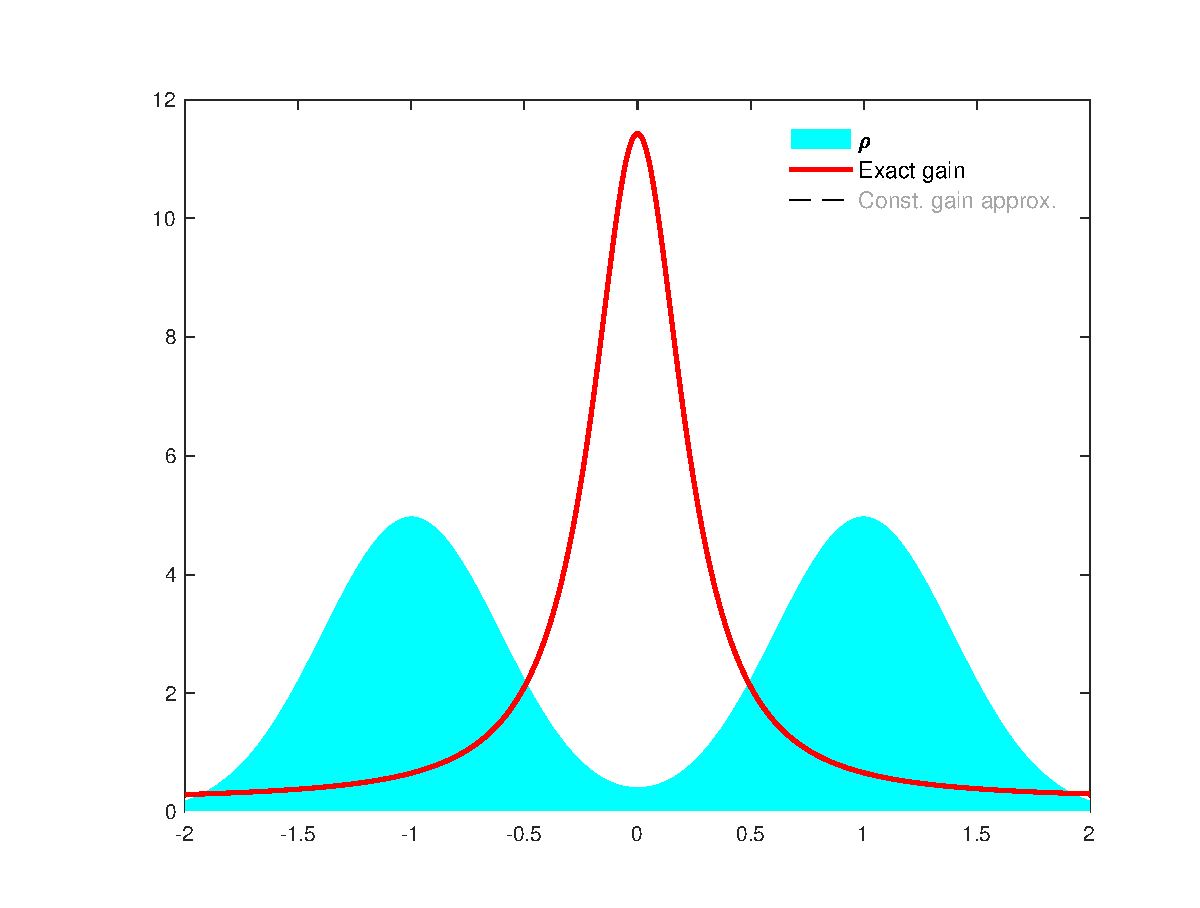
\includegraphics[width= .65\hsize]{gain_exact.eps}}
%		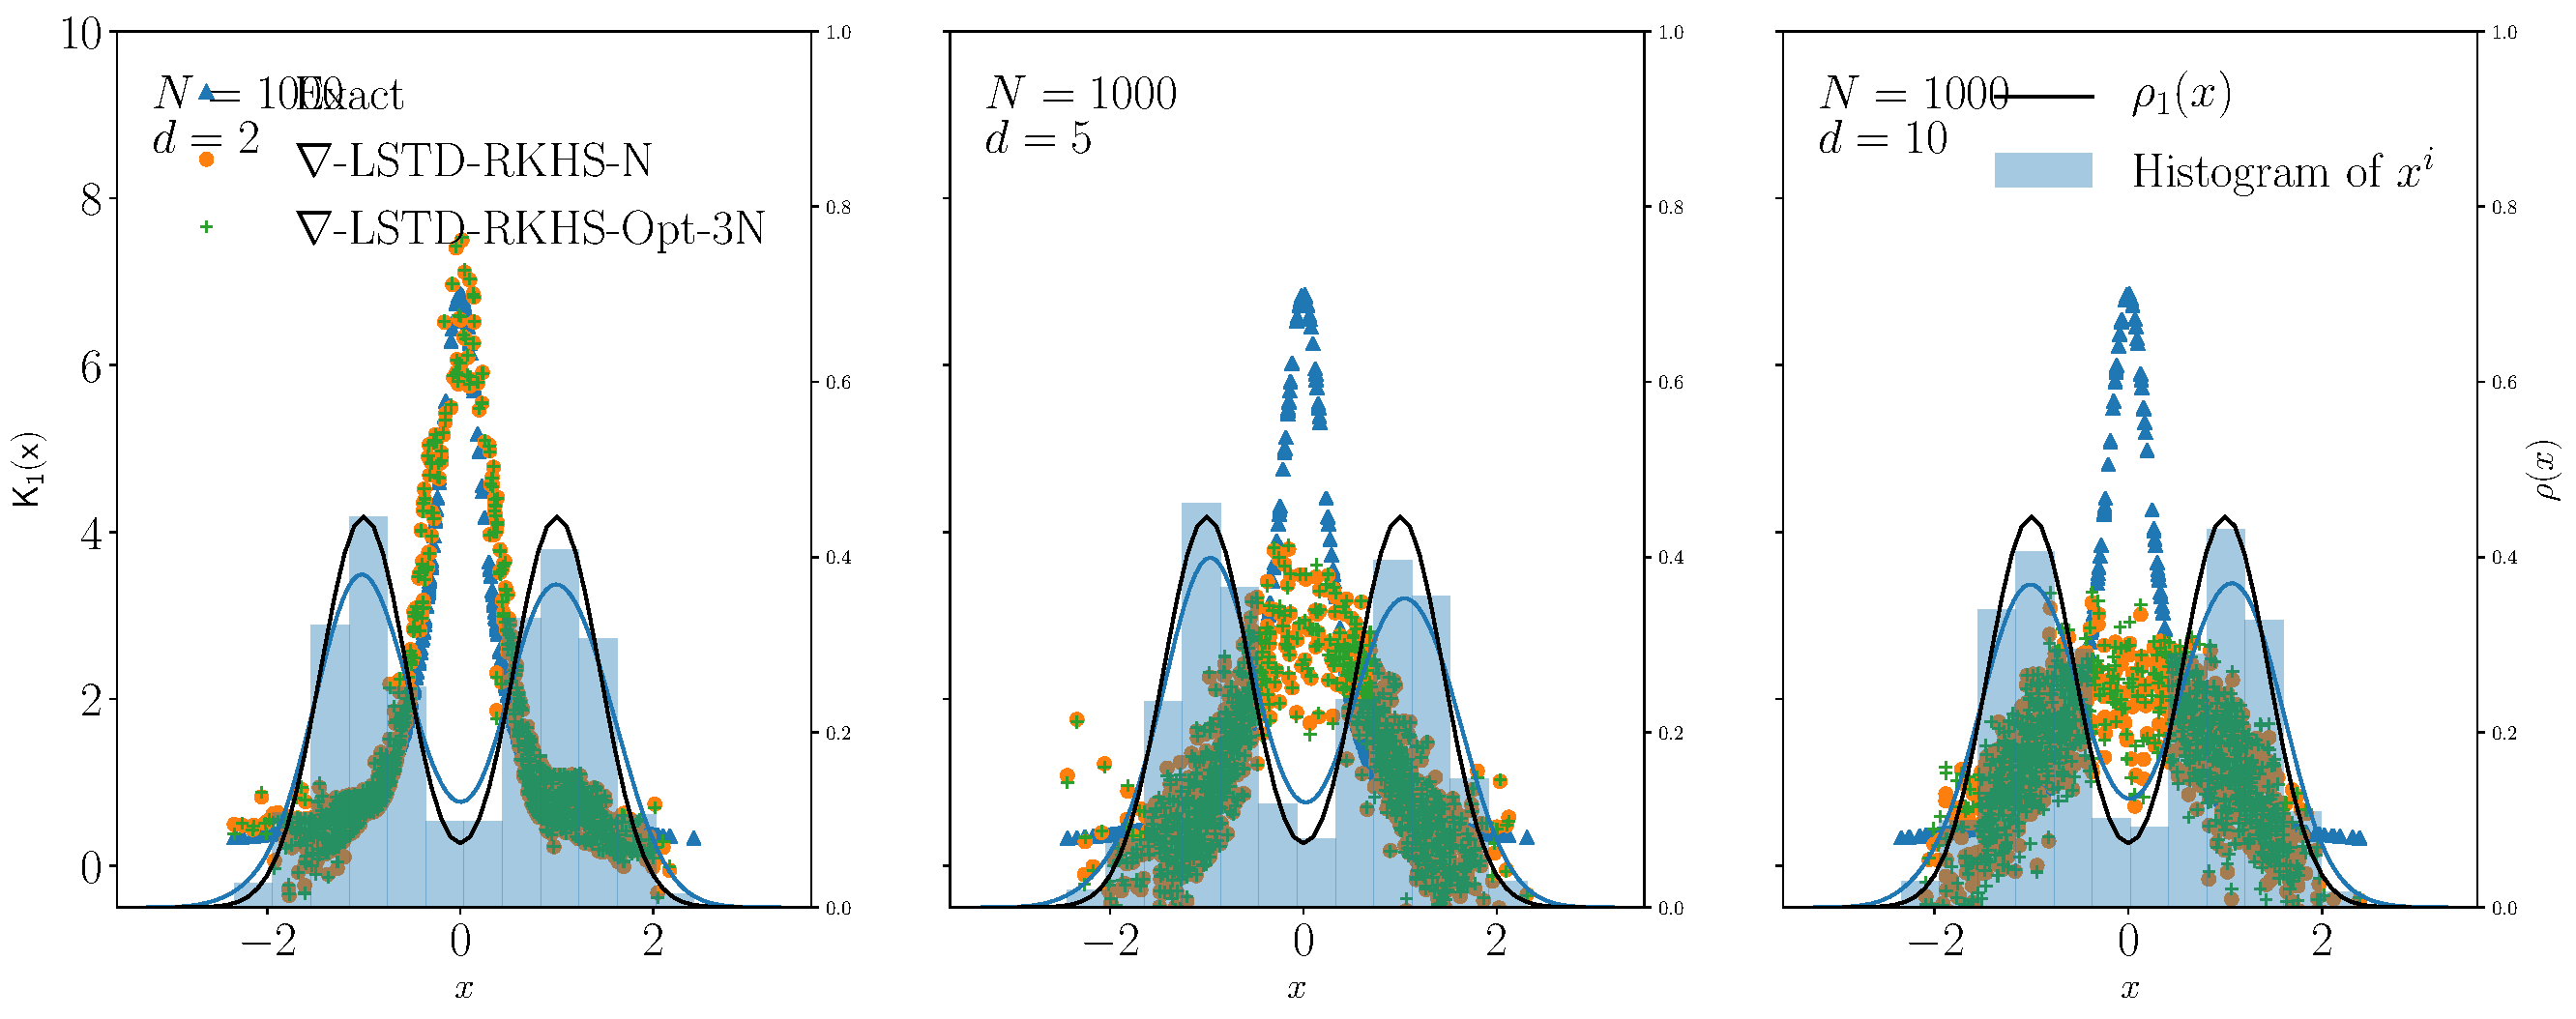
\includegraphics[width= \hsize]{Chap4_gain_N_dN_d2510.pdf}\\
%		$\gradTD$-RKHS-N and $\gradTD$-RKHS-Optimal
%	}

	\only<1>{
		\centering 
		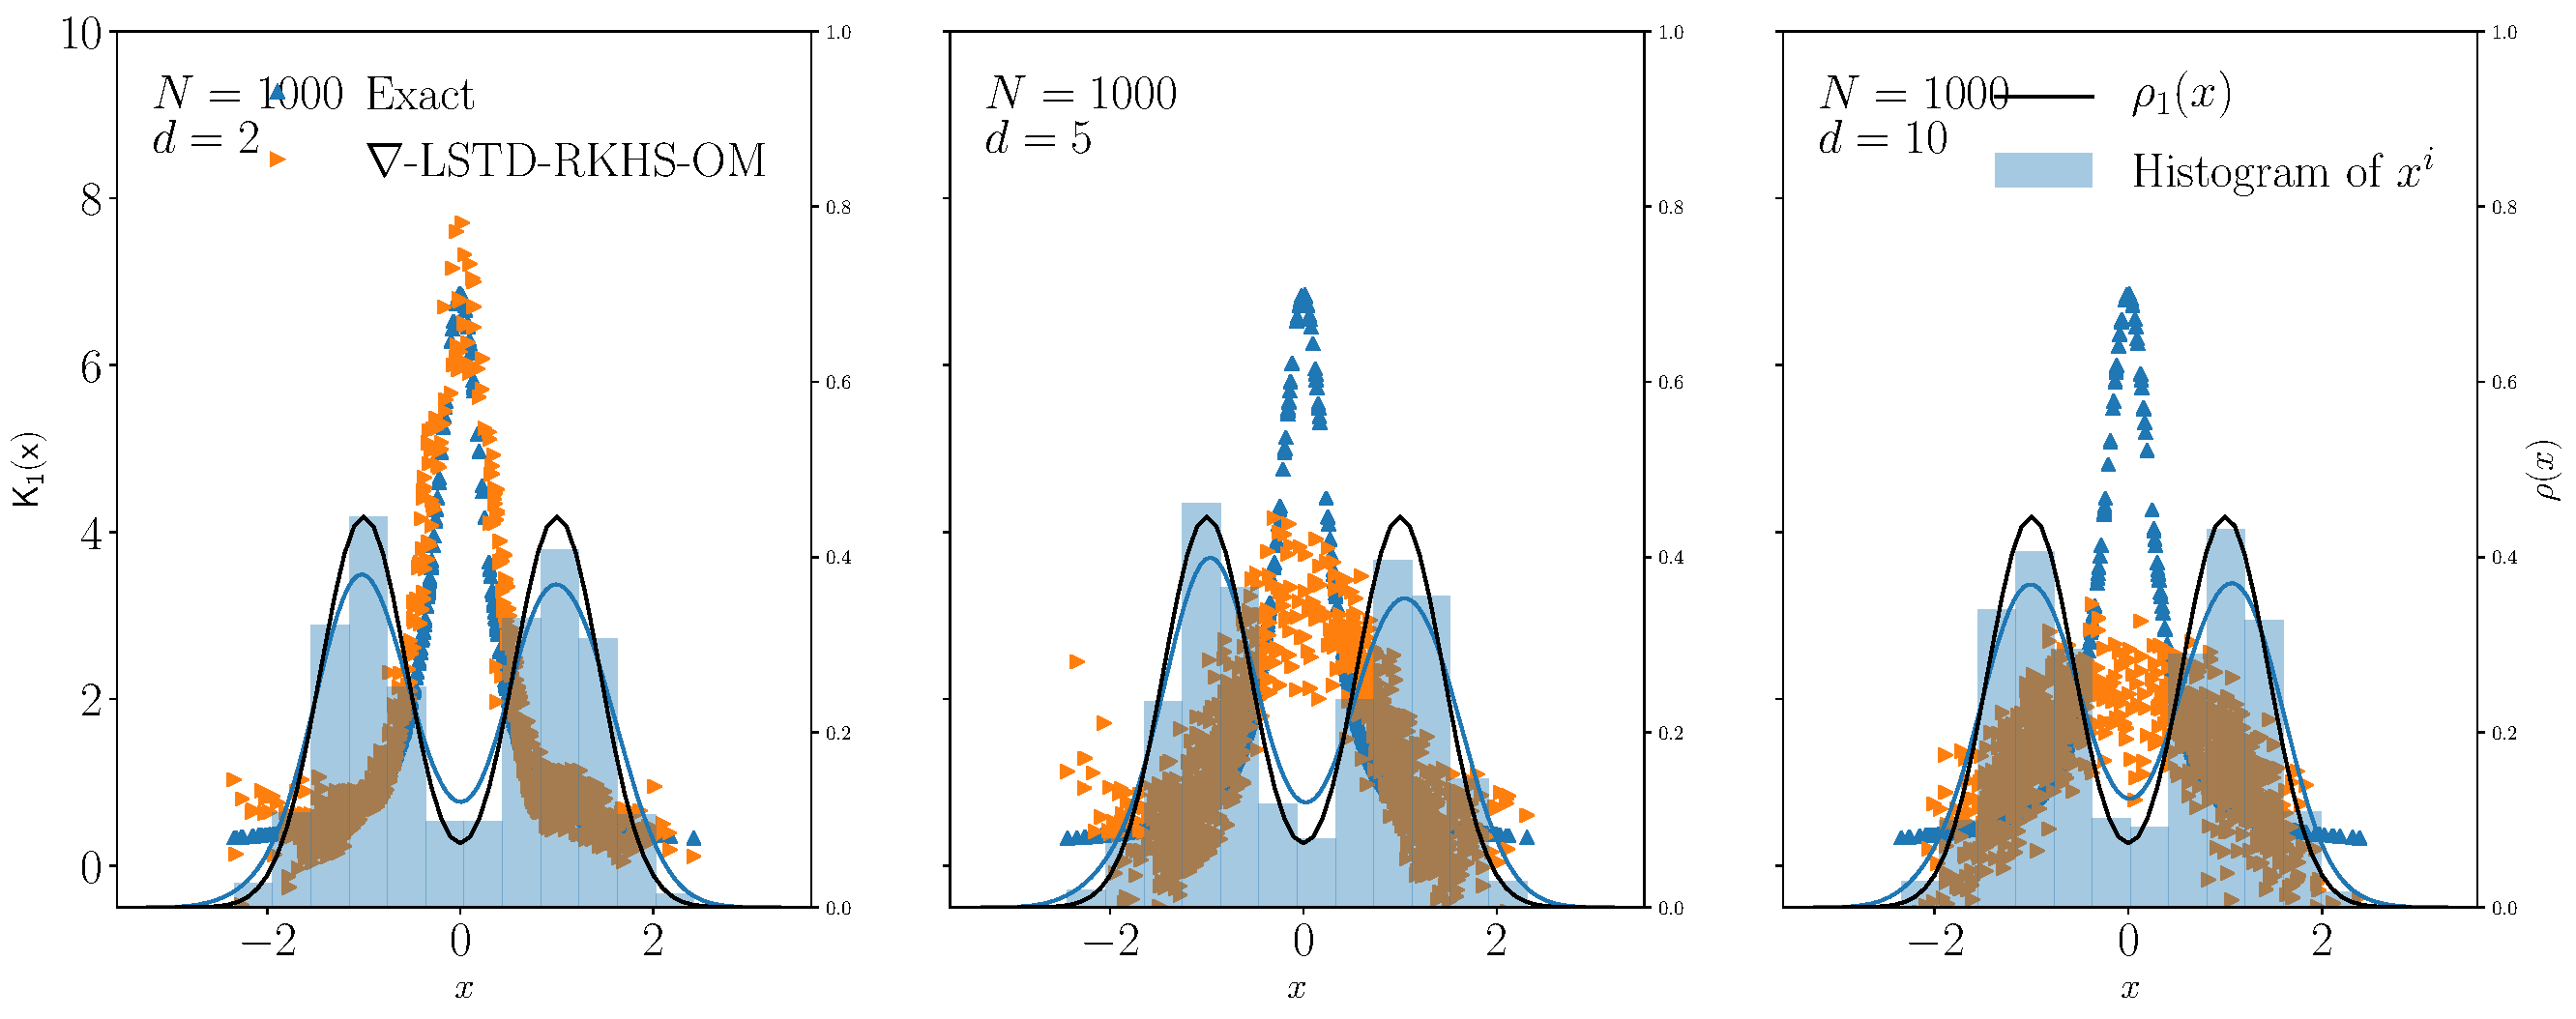
\includegraphics[width=\hsize]{Chap4_gain_om_d2510.pdf}\\
		$\gradTD$-RKHS-OM
	}

	\only<2>{
		\centering
		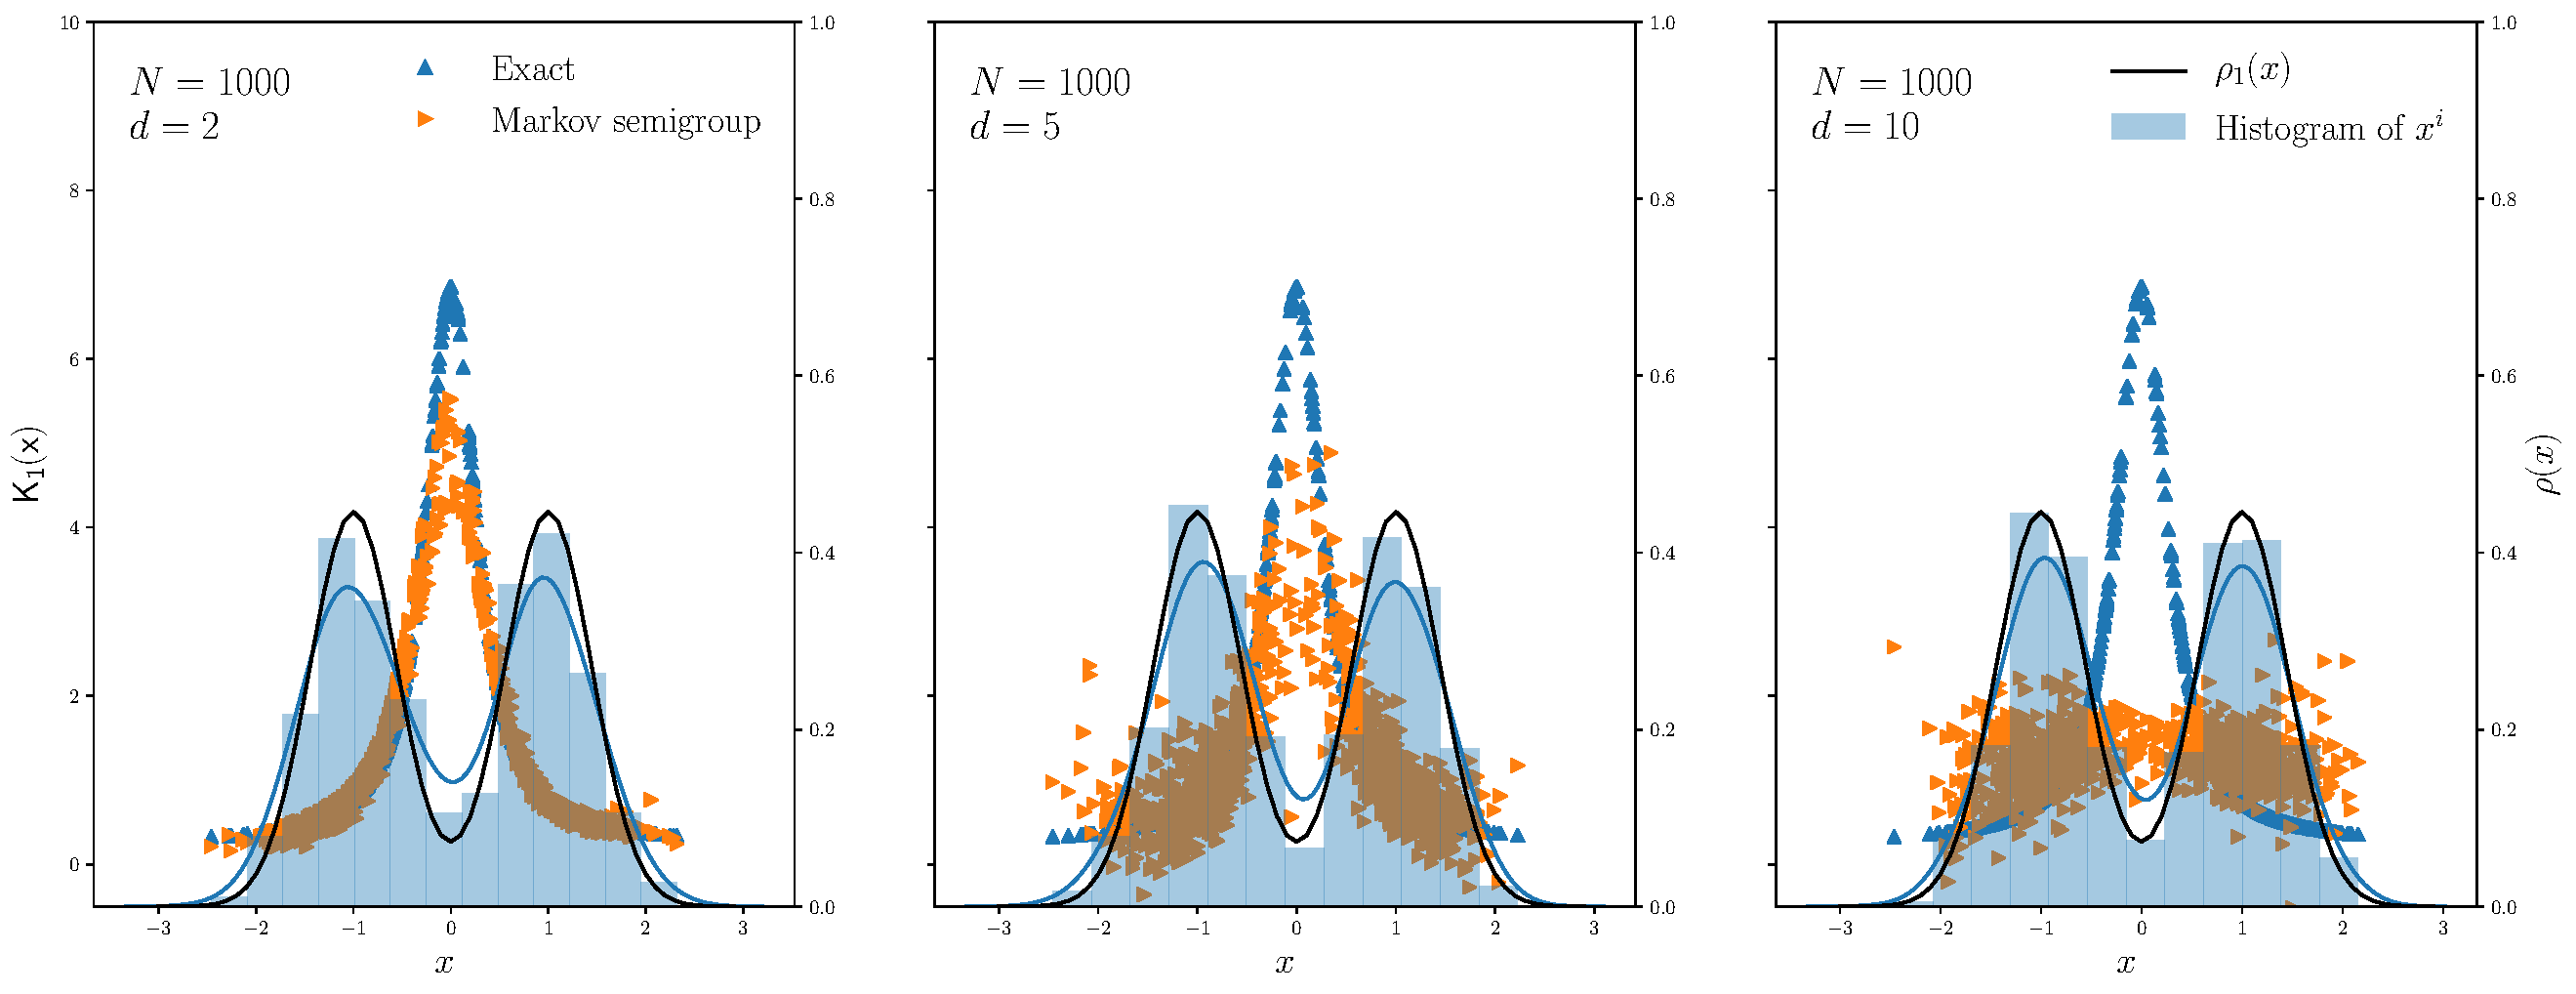
\includegraphics[width= \hsize]{Chap4_gain_coif_d2510.pdf}\\
		Markov kernel approximation
	}
\end{minipage}
\end{frame}

\begin{frame}
\frametitle{Application to nonlinear filtering}
\framesubtitle{Numerical example - Gain for a nonlinear oscillator model}
\begin{minipage}[t][6.5cm][t]{\textwidth}
	\begin{tabular}{lll}\alertb{Example:} 
	& $\pr(x)$ is a mixture of von Mises densities on a circle \\
	& $\ud \oscState = \omega \ud t+\sigma_{B}\ud B_t \quad \text{mod }2\pi$,	\\
	& $\ud Z_t = c(\oscState)\ud t+ \sigma_{W} \ud  W_t, \quad c(\oscState)=\frac{1}{2}[1+\cos(\oscState)]$
\end{tabular}
	
	\only<2>{
		\centering
		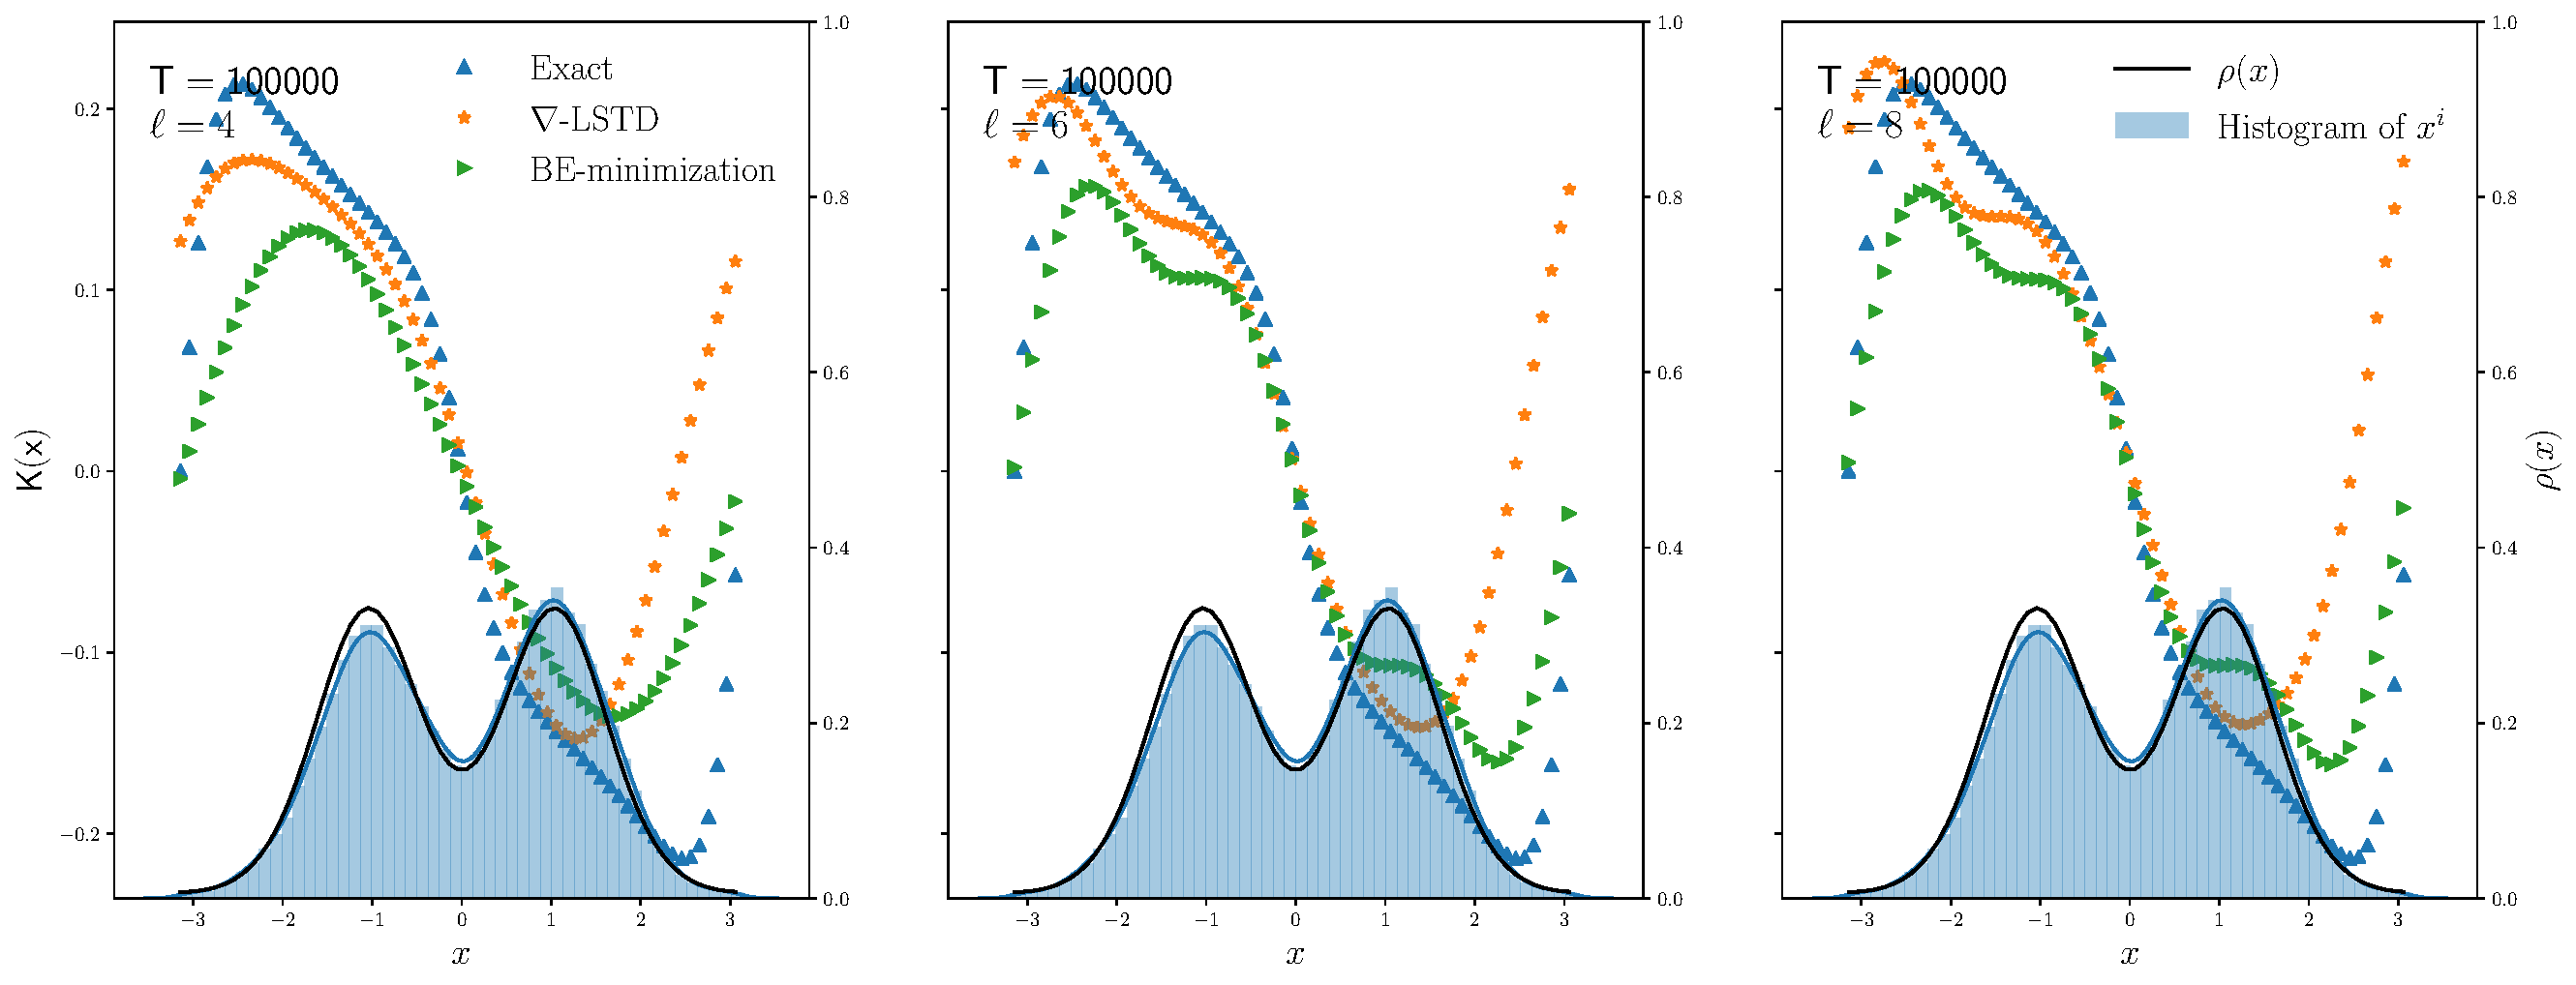
\includegraphics[width= \hsize]{Chap4_nl_oscillator_be.pdf}\\
		$\gradTD$-L with $\basis_i = \sin(ix), \basis_{i+1} = \cos(ix)$ with $1 \leq i \leq \ell/2$, $\ell = 4,6,8$.
	}
	
\end{minipage}
\end{frame}

\begin{frame}
\frametitle{Applications to Nonlinear filtering}
\framesubtitle{Numerical example - Parameter estimation}
\begin{minipage}[t][6.5cm][t]{\textwidth}
	
	\begin{tabular}{lll}\alertb{Example:}   & Parameter estimation with bimodal prior 
		\\
		&   Observations:  parameter plus additive noise with $\sigma_W = 1$.
	\end{tabular}

	\centering
	\only<1>{ 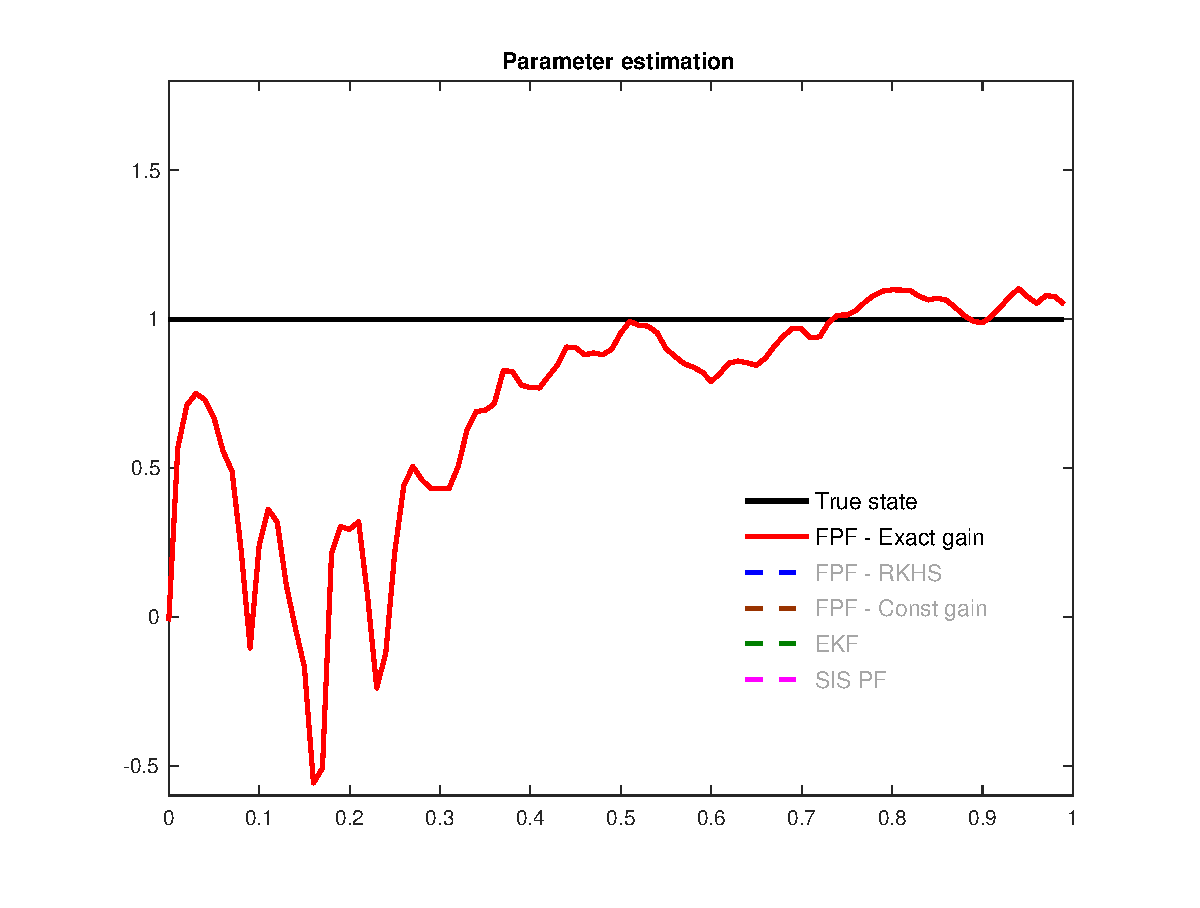
\includegraphics[width= .7\hsize]{state_est_exact.eps}  	
	}	
	\only<2>{ 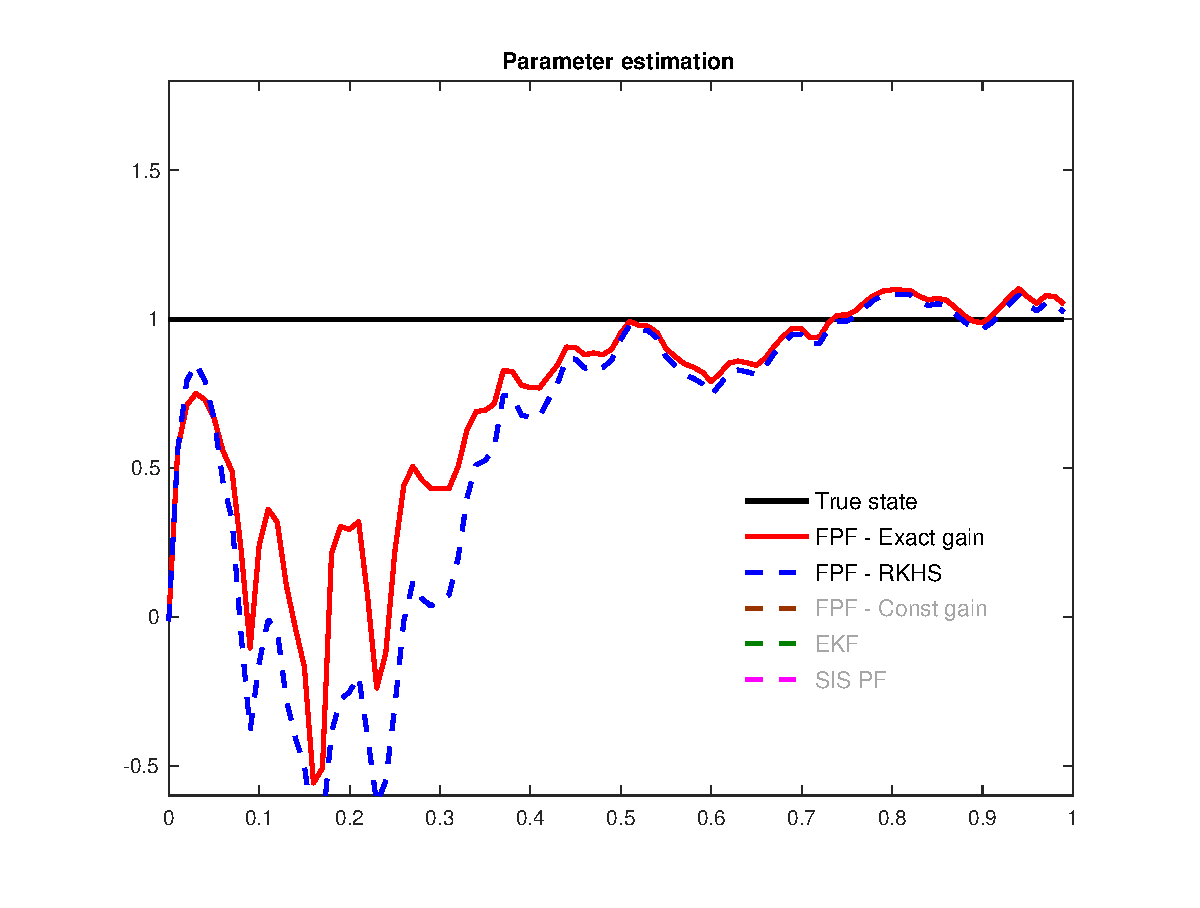
\includegraphics[width= .7\hsize]{state_est_rkhs.eps}  	
	}	
	\only<3>{	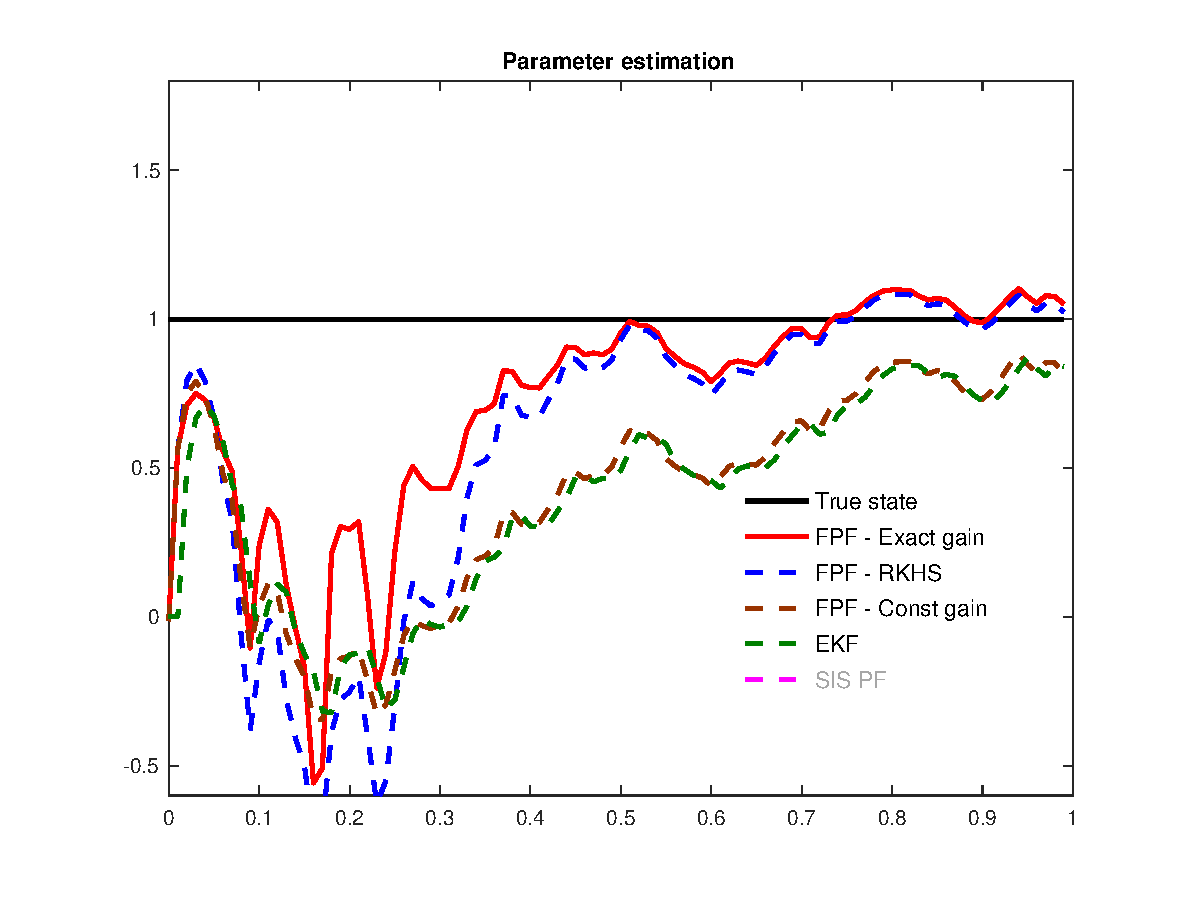
\includegraphics[width= .7\hsize]{state_est_const_kal.eps}}
	\only<4->{	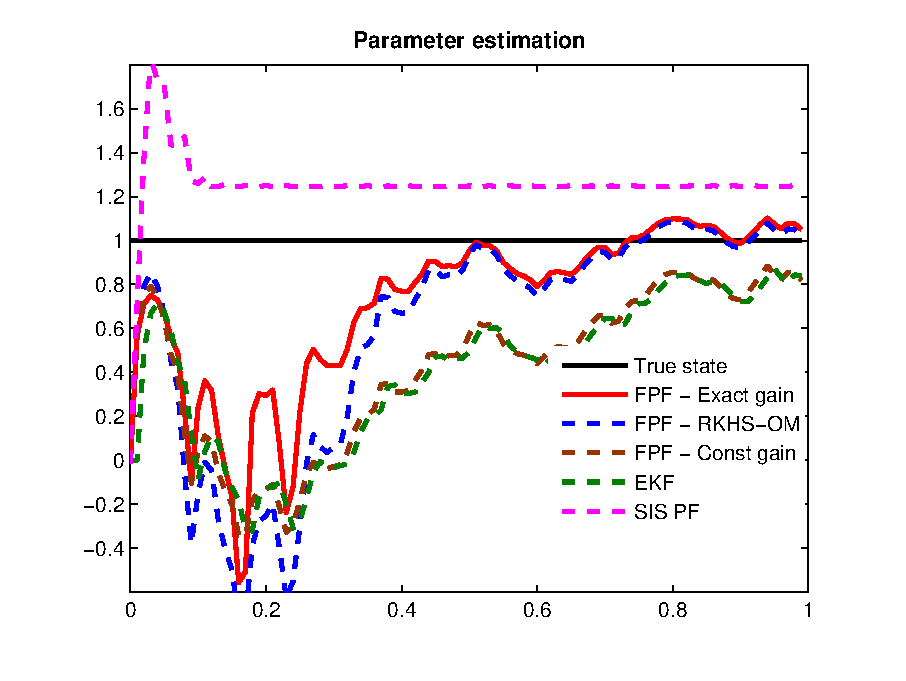
\includegraphics[width= .7\hsize]{state_est_all.eps}}
\end{minipage}
\end{frame}

\begin{frame}
\frametitle{Applications to Nonlinear filtering}
\framesubtitle{Numerical example - Parameter estimation}
\begin{minipage}[t][6.5cm][t]{\textwidth}
	
	\begin{tabular}{lll}\alertb{Example:}   & Parameter estimation with bimodal prior
		\\
		&   Observations:  parameter plus additive noise with $\sigma_W = 1$.
	\end{tabular}
  \begin{figure}
  	\centering
%  	\mbox{
%  		\subfloat [] {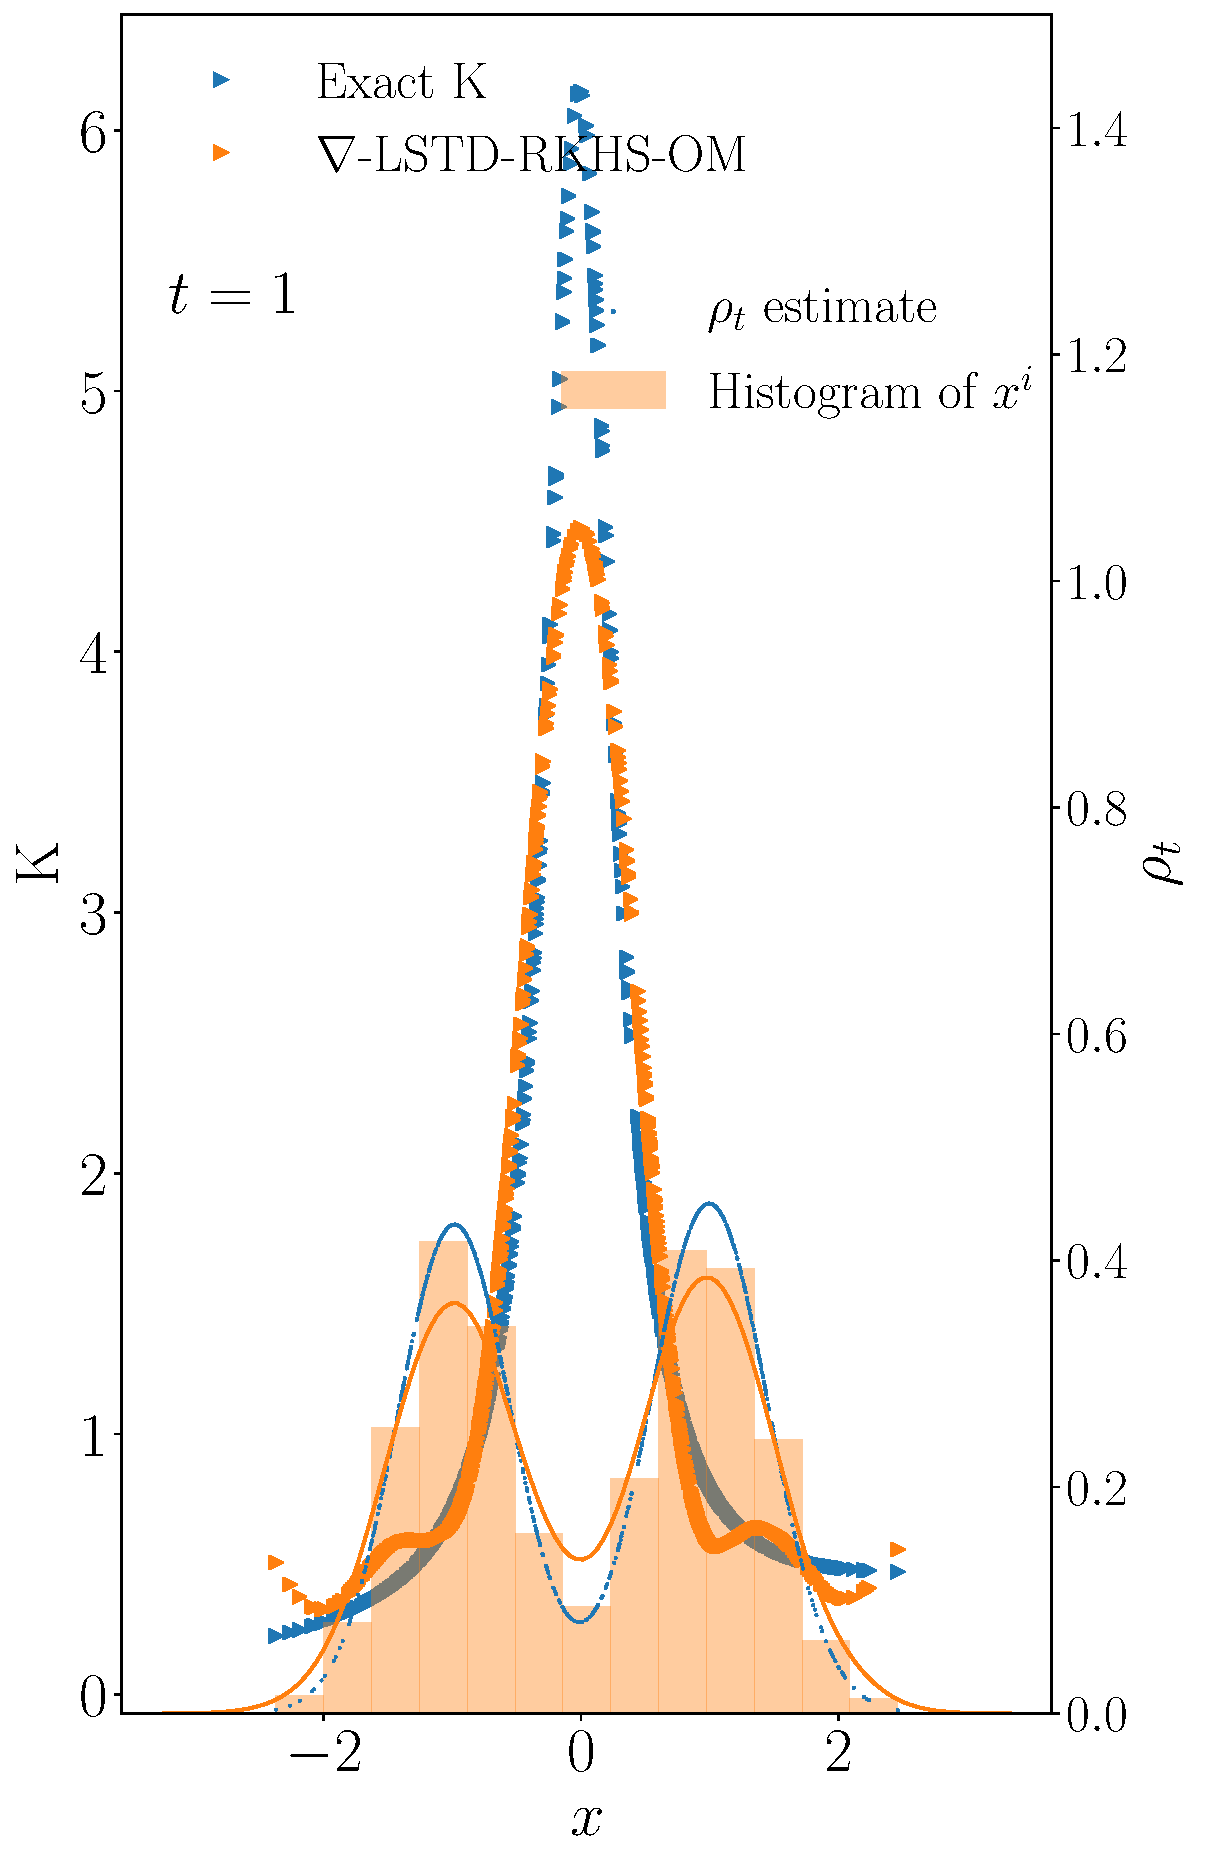
\includegraphics[width = 0.3\hsize]{Chap4_gain_posterior_exact_om_t_1.pdf}} 
%  		\subfloat [] {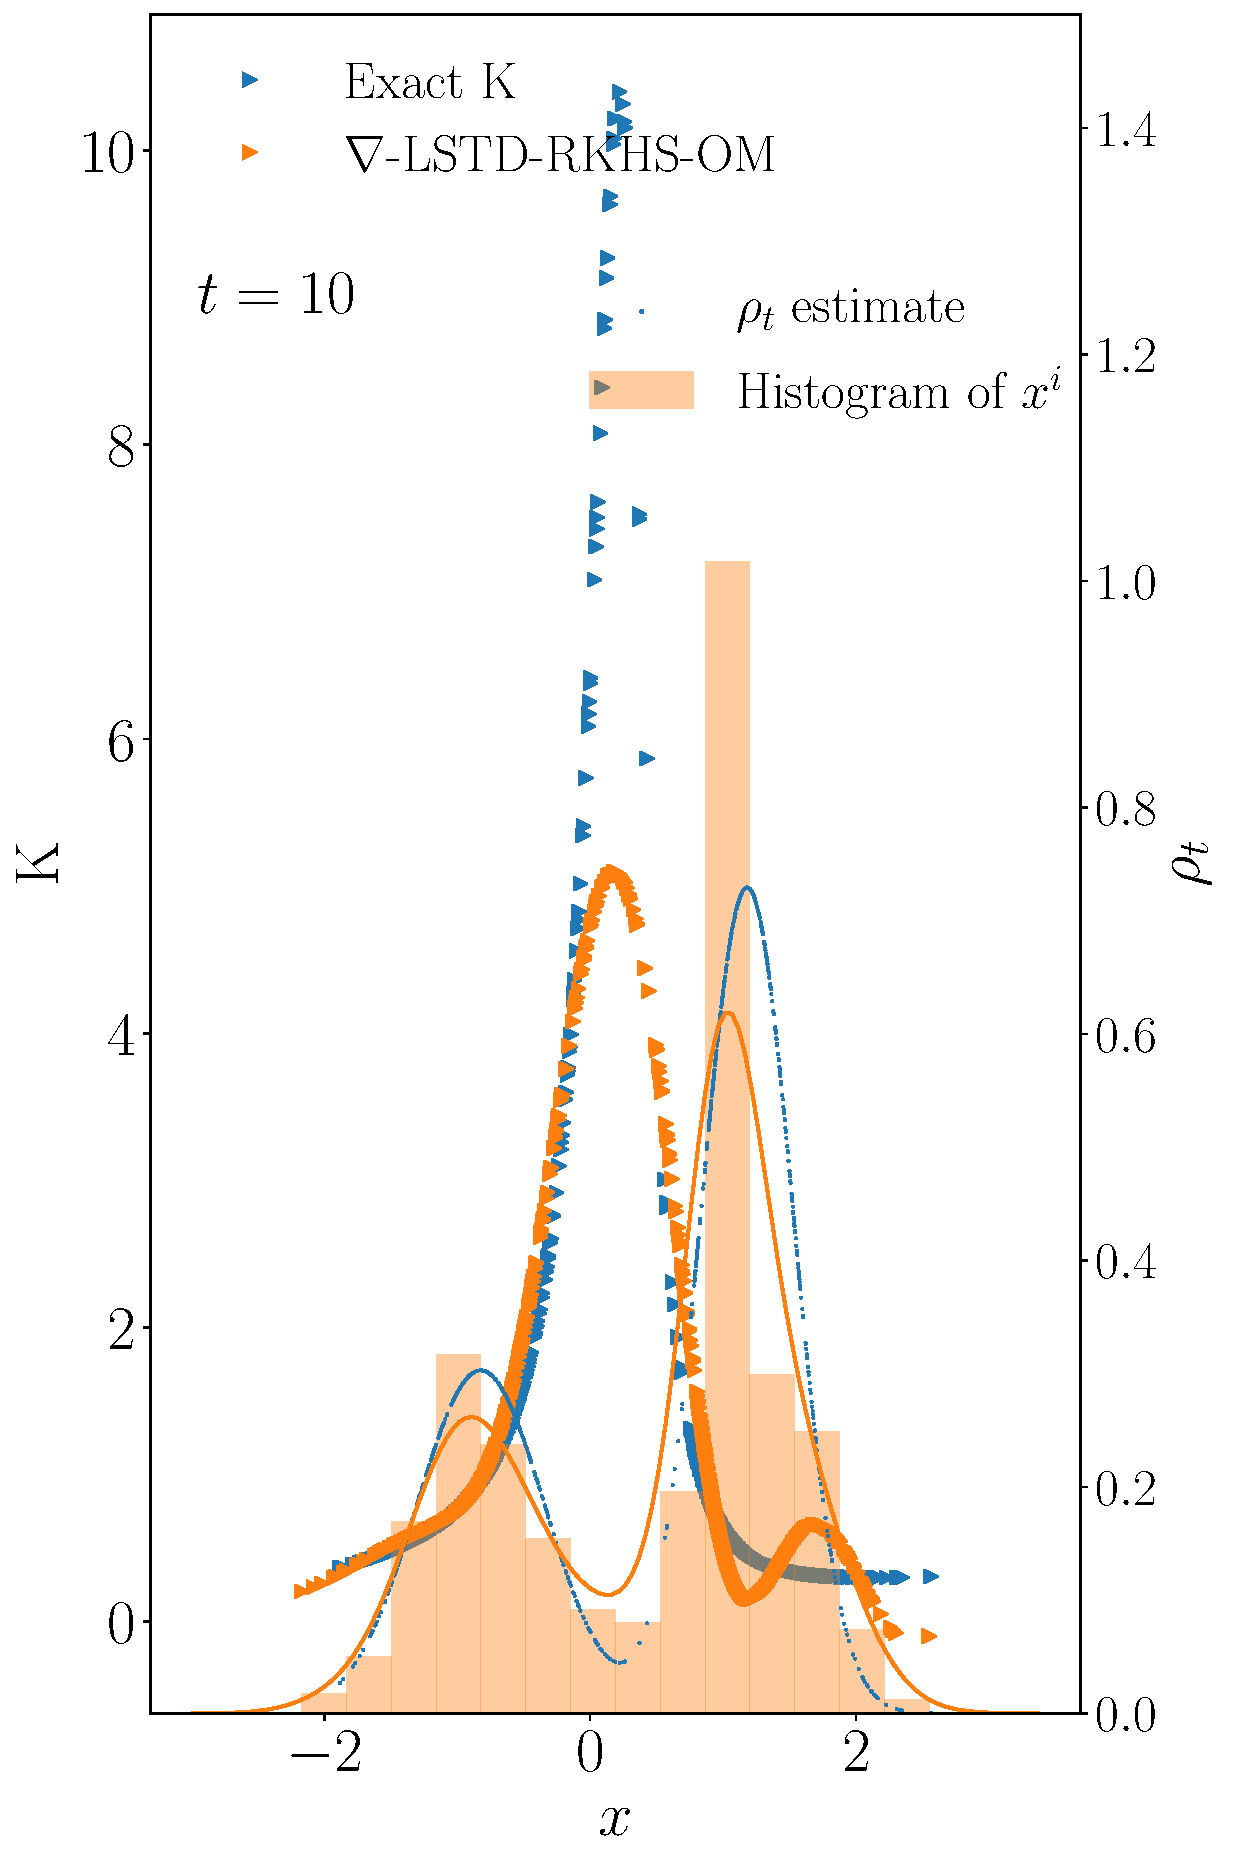
\includegraphics[width= 0.3\hsize]{Chap4_gain_posterior_exact_om_t_10.pdf}} 
%  		\subfloat [] {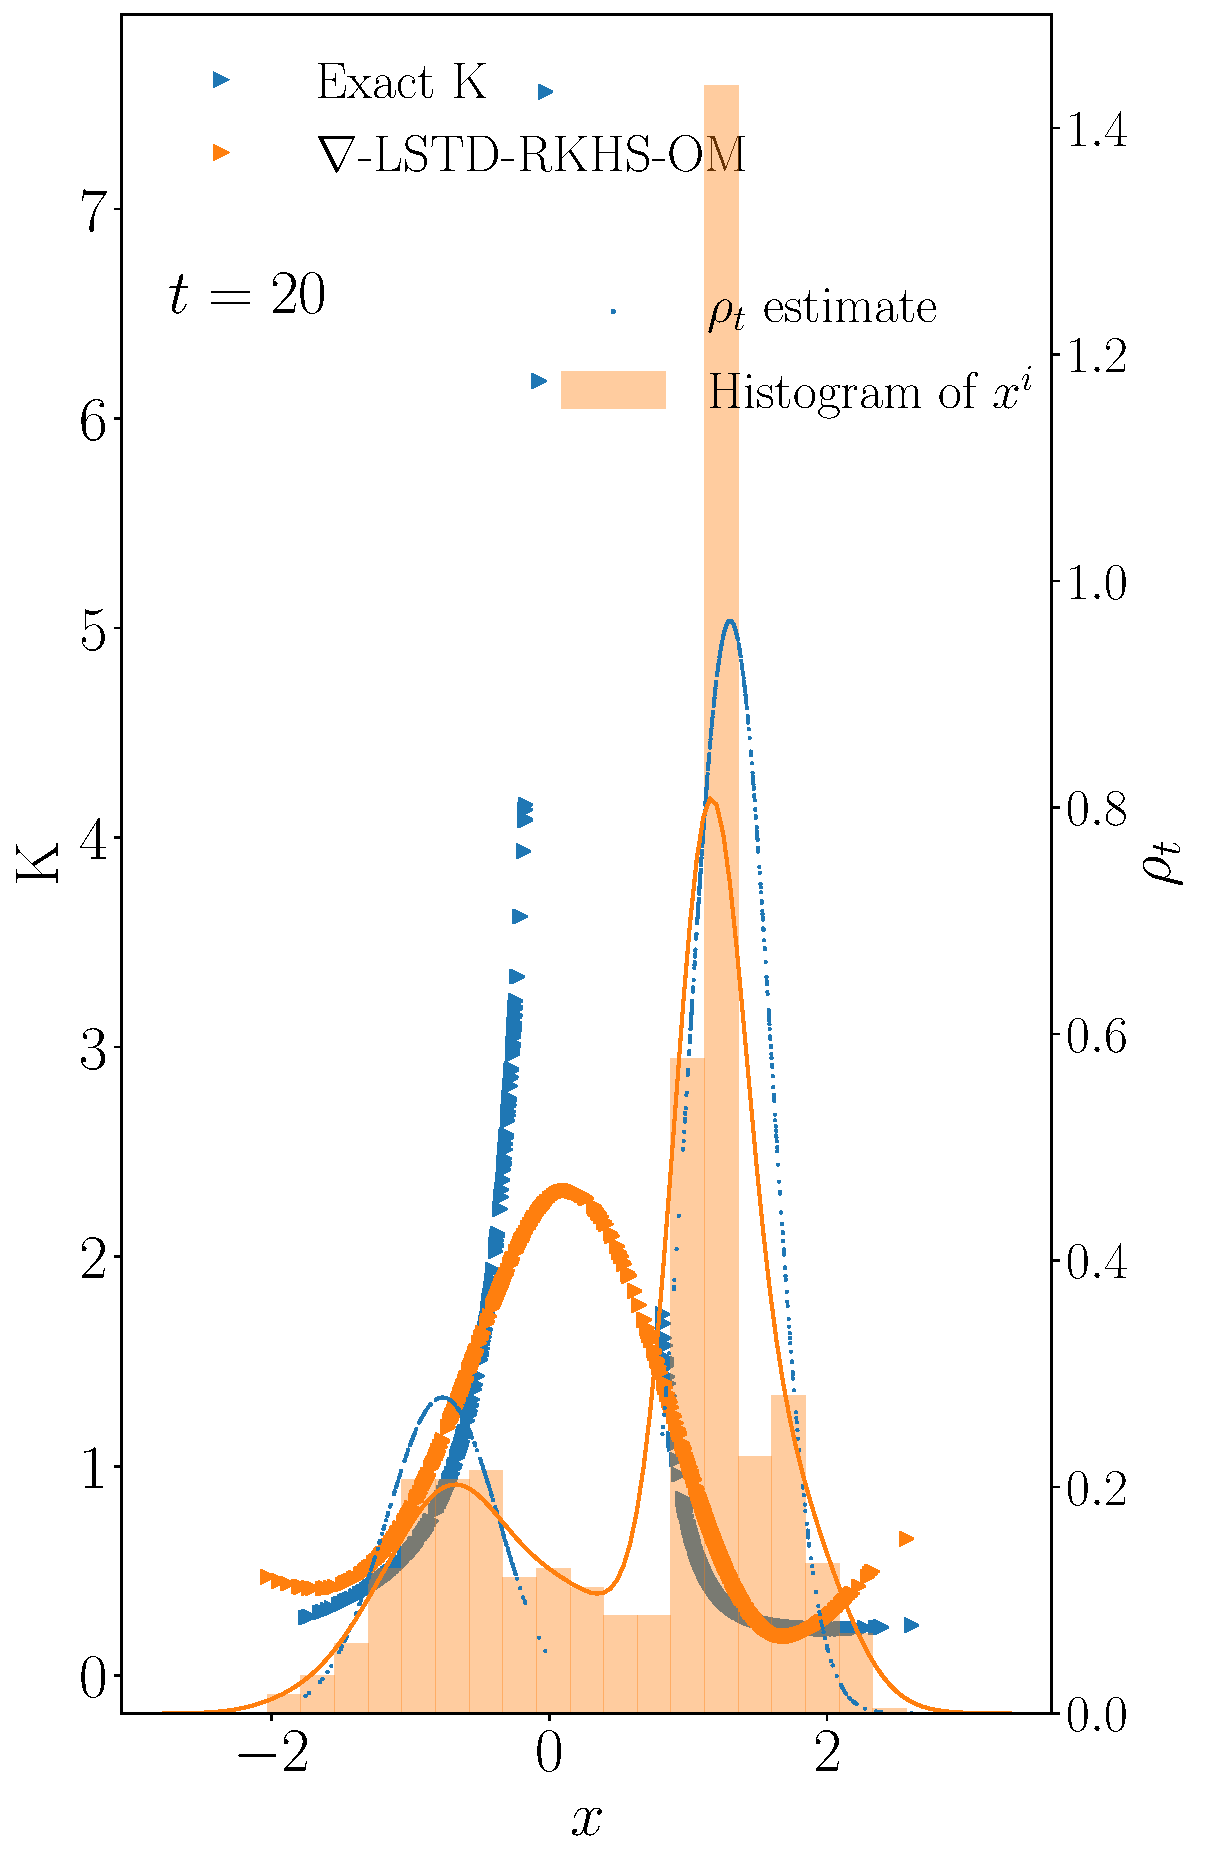
\includegraphics[width = 0.3\hsize]{Chap4_gain_posterior_exact_om_t_20.pdf}} 
%  	}
	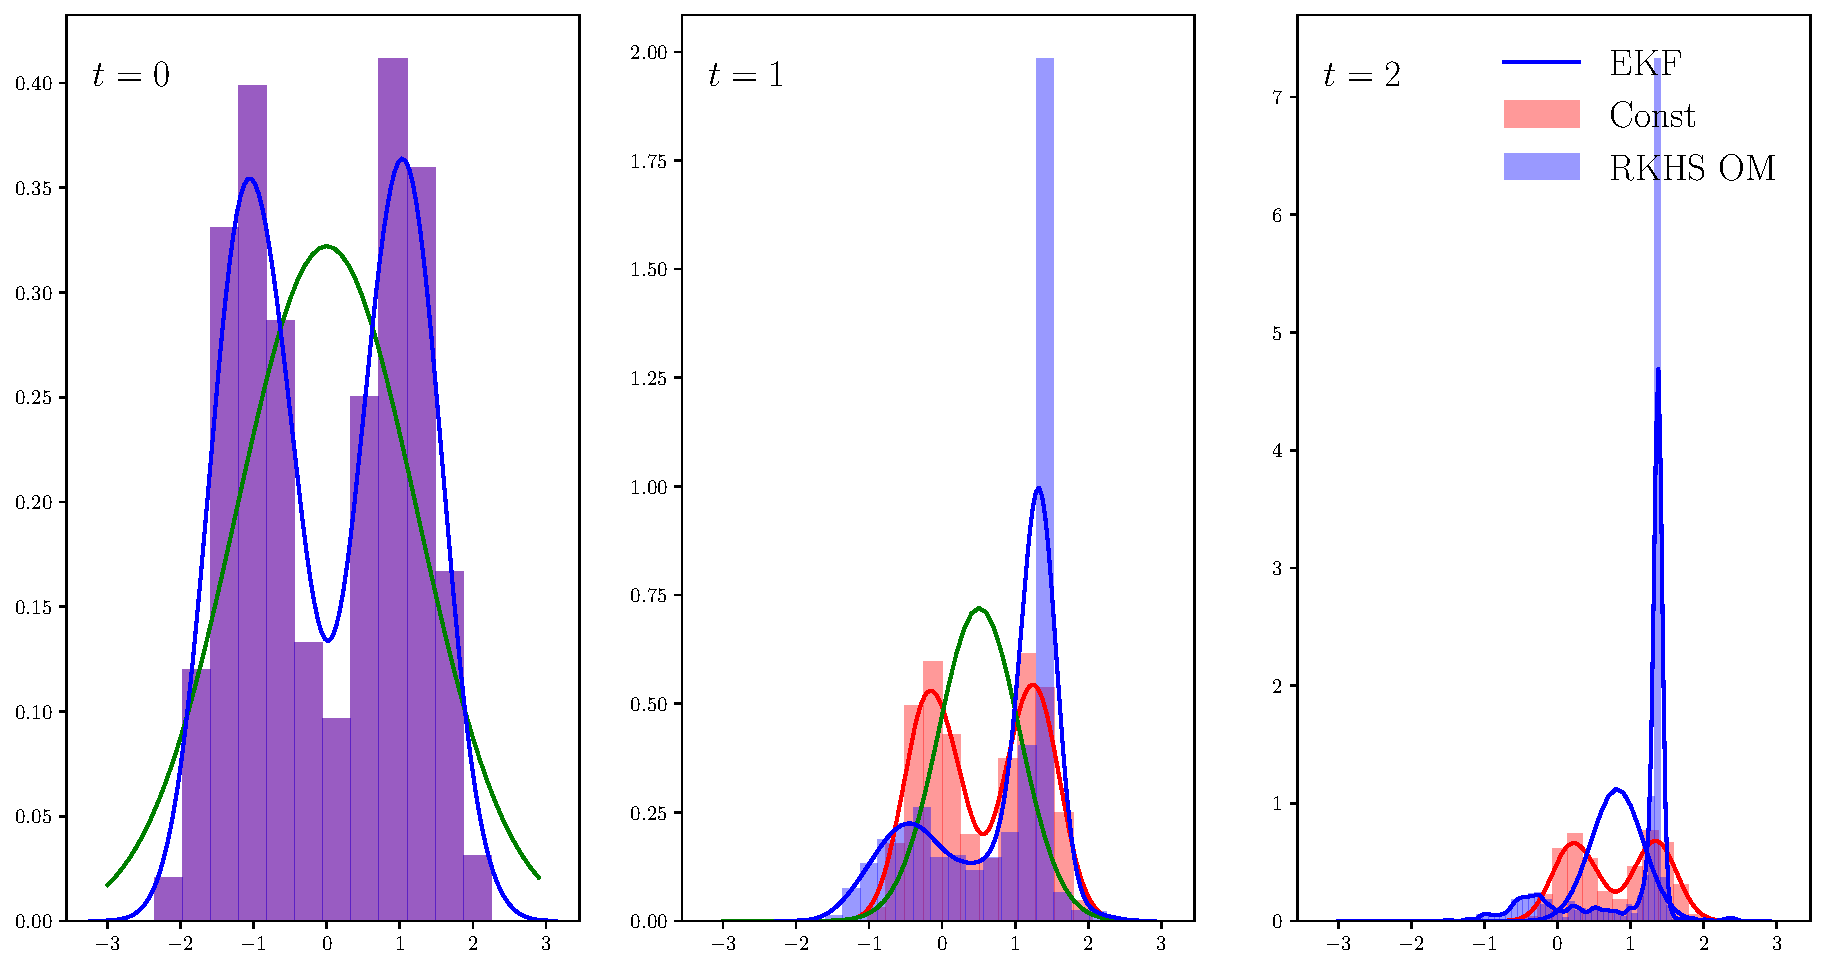
\includegraphics[width = 0.85\hsize] {Chap4_Posterior_estimate.pdf}
  \end{figure}
\end{minipage}
\end{frame}

\begin{frame}
\frametitle{Applications to Nonlinear filtering}
\framesubtitle{Numerical example - Nonlinear $2d$ ship dynamics model}
\begin{minipage}[t][6.5cm][t]{\textwidth}
	
	\begin{tabular}{lll}\alertb{Example:}   & Nonlinear ship dynamics model in $2d$.
		\\
		&   Observations: $c(x) = \arctan(x_1/x_2)$ with std. deviation  $ \approx 18^\circ$.
	\end{tabular}
	
	
	\centering
	\only<1>{ 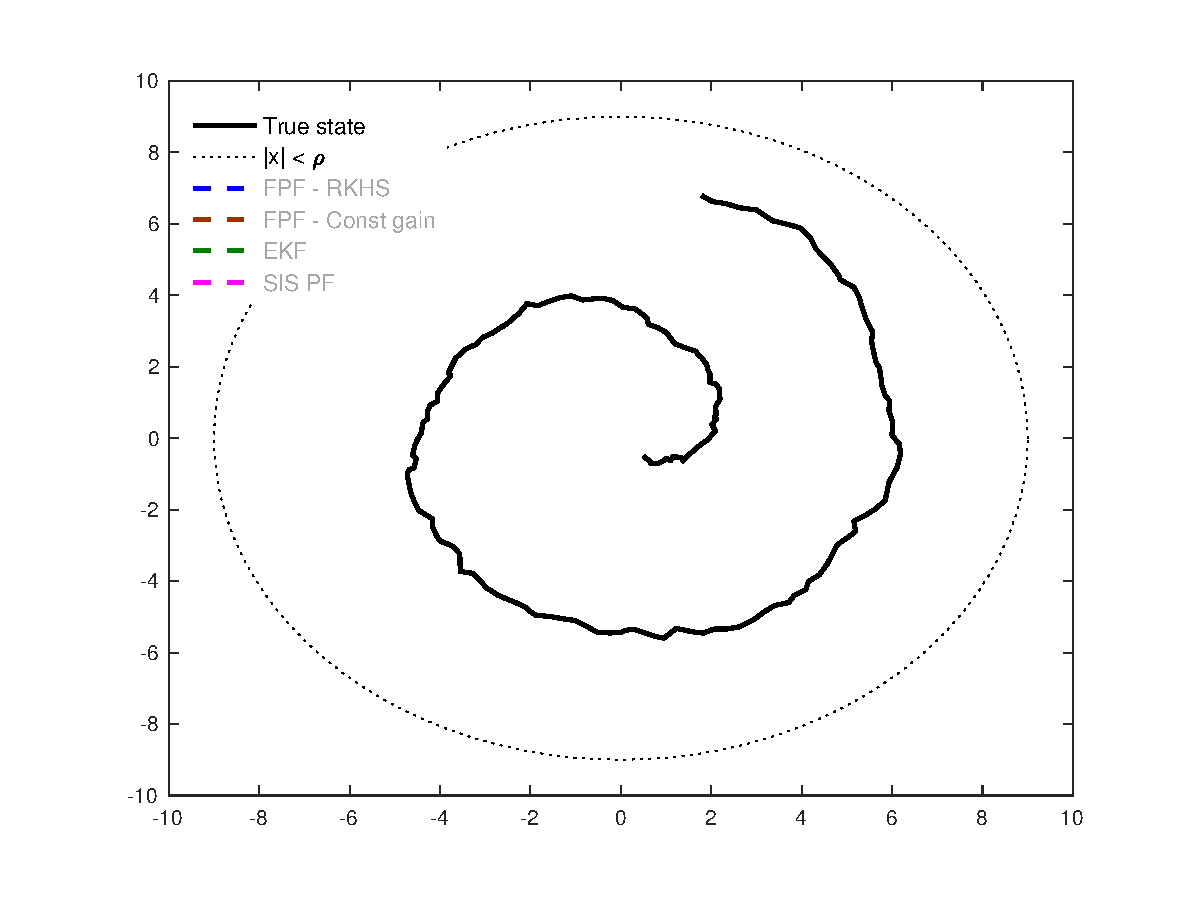
\includegraphics[width= .6\hsize]{ship_state_exact.eps}  	
	}	
	\only<2>{ 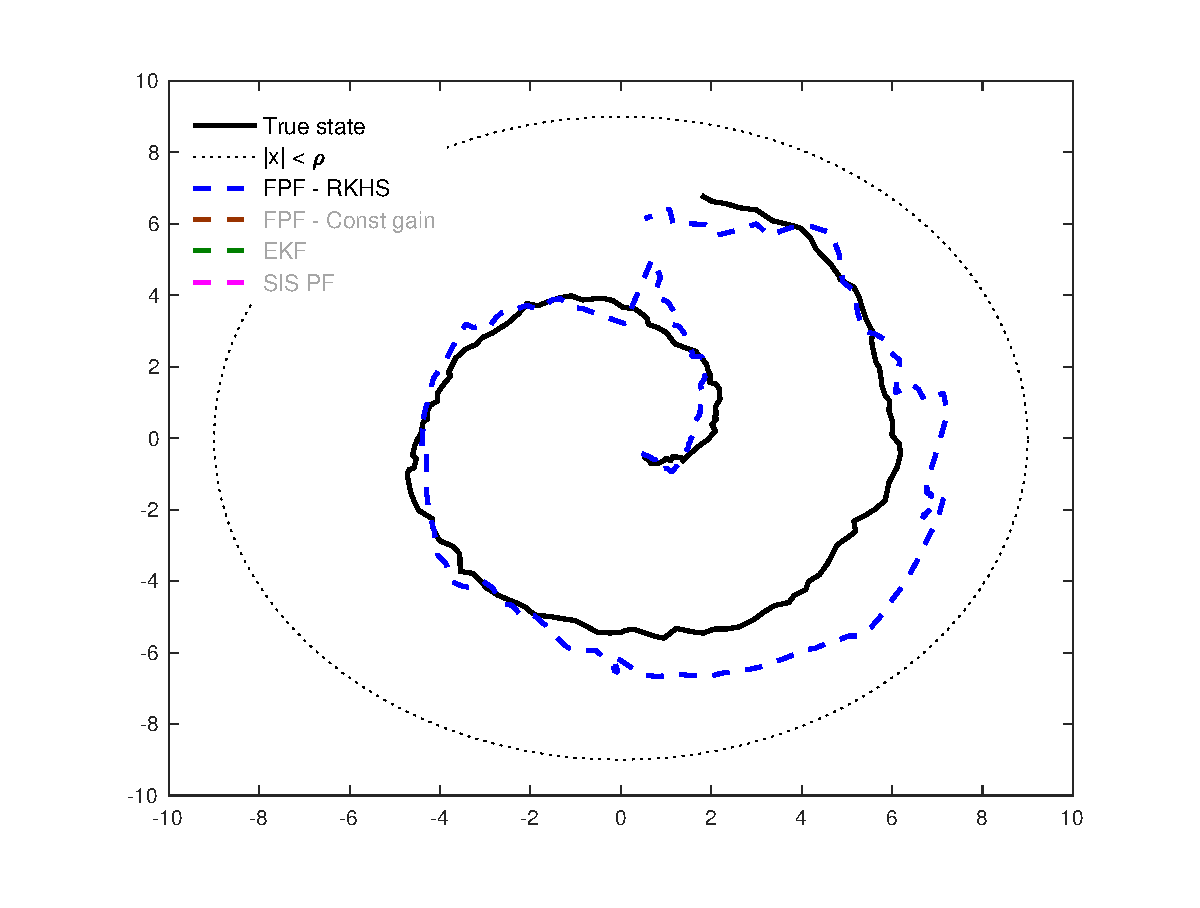
\includegraphics[width= .6\hsize]{ship_state_rkhs.eps}  	
	}	
	\only<3>{	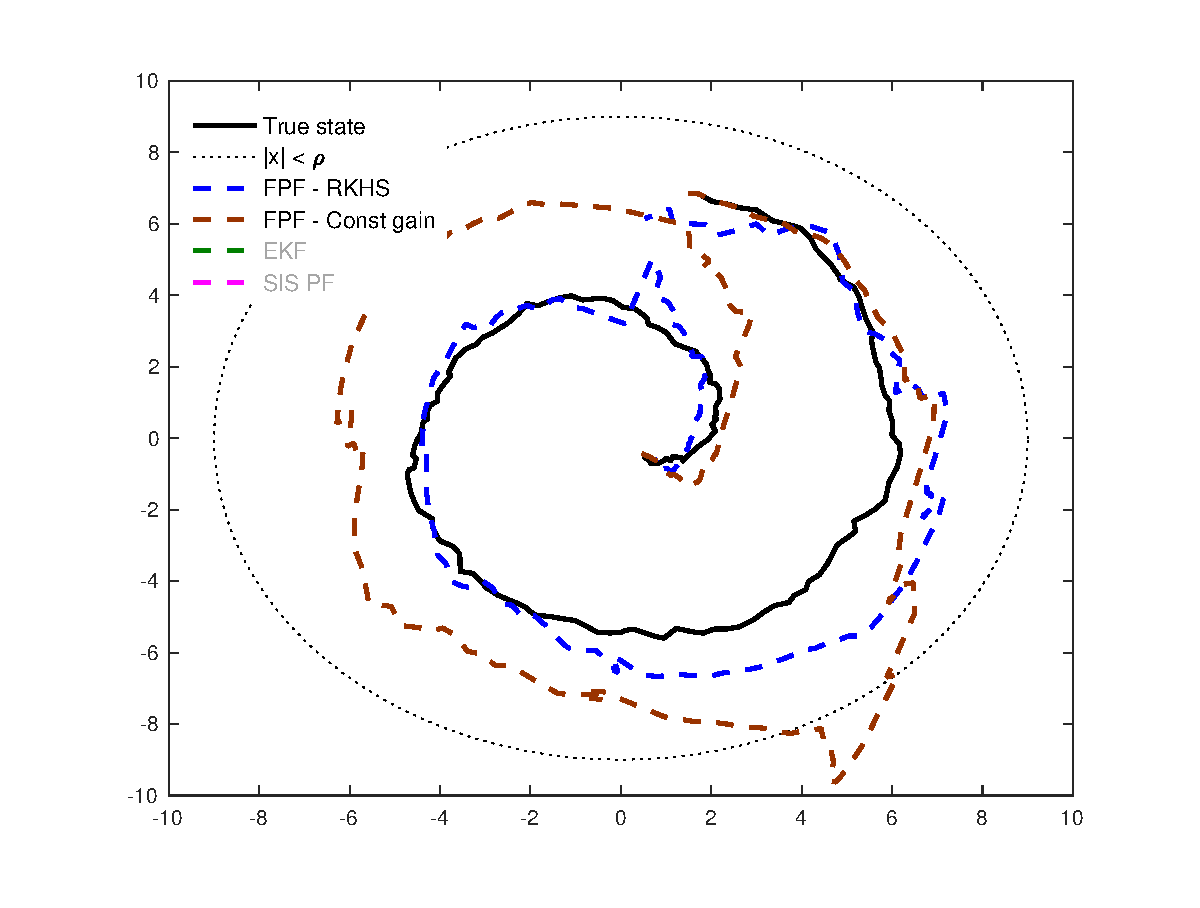
\includegraphics[width= .6\hsize]{ship_state_const.eps}}
	\only<4->{	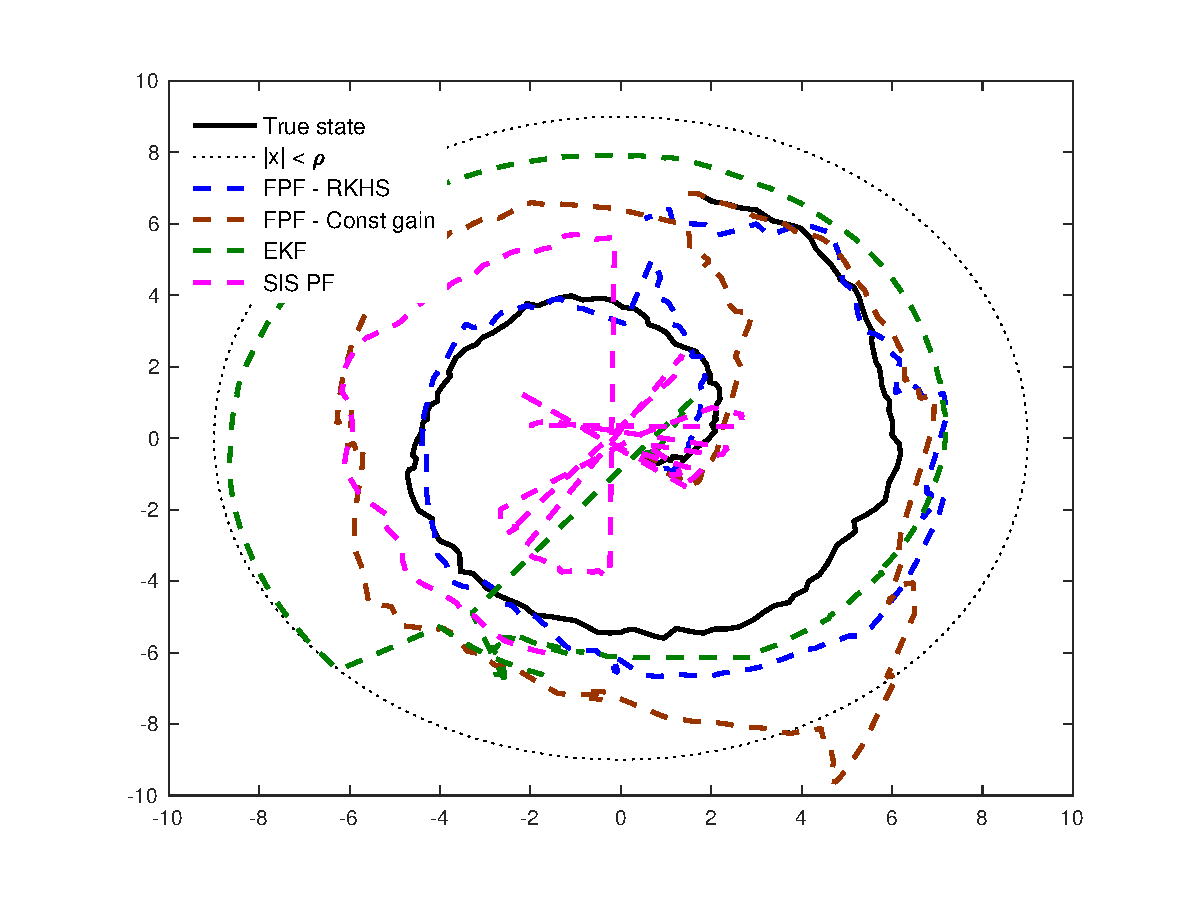
\includegraphics[width= .6\hsize]{ship_state_all.eps}}
\end{minipage}
\end{frame}

\begin{frame}
\frametitle{Applications to Nonlinear filtering}
\framesubtitle{Numerical example - Nonlinear $2d$ ship dynamics model}
\begin{center}
	\centering Summary table of RMSEs from $100$ trials	\begin{tabular}{ |c|c|c|c| }
		\hline
		Type of filter & $\Sigma_1 = I_{2 \times 2}$ & $\Sigma_2 = 5I_{2 \times 2}$ & Lost track ($\Sigma_2$) \\
		\hline
		FPF RKHS-OM & $0.9023$  &  $1.6254$ & $4$ times\\
		FPF RKHS mem. &$0.9162$ &  $ 1.9408$ & $ 7 $ times\\
		FPF const. gain & $1.3060$ & $2.3231$ & $14$ times \\
		SIR PF & $3.1481$  &  $4.2648$ &  $57$ times \\
		EKF &  $6.5203$ & $18.441$ & $93$ times \\ 		
		\hline
	\end{tabular}
\end{center}
\end{frame}

\section{Applications to MCMC}
\begin{frame}
\frametitle{Applications to MCMC}
\framesubtitle{Introduction to MCMC}
In many applications, we need to compute
\begin{equation*}
\eta = \int c(x)\pr(x) \rmd x
\label{e:eta}
\end{equation*}
\begin{itemize}
	\item $c\colon\Re^\ell\to\Re$ is a measurable function.
	\item $\pr$ is a target probability density in $\Re^\ell$.
\end{itemize}
 Markov-Chain Monte Carlo (MCMC) methods provide numerical algorithms to obtain estimates:
	\[
	\eta_t =\frac{1}{t}\int_0^t c(\markovstate(s)) \, ds
	\label{e:sample_mean}
	\]
\begin{center}
	$\bfPhi$ is a Markov process with steady state distribution $\pr$.
\end{center}
\end{frame}

\begin{frame}
\frametitle{Applications to MCMC}
\framesubtitle{Asymptotic Variance}
Estimates $\eta_t$ obey a Central Limit Theorem,
\[
\sqrt{t} (\eta_t - \eta) \xrightarrow[]{d} N(0,\gamma^2)
\]

Rate of convergence captured by \alertb{asymptotic variance}
\[
\gamma^2 = \lim_{t \to \infty} \Expect \left[\left(\frac{1}{\sqrt{t}}\int_{0}^{t}(c(\markovstate(s))-\eta)\,ds\right)^2\right]
\]
Alternate representation in terms of covariance
\[
\gamma^2  \eqdef \int_{-\infty}^\infty R(s) ds, \qquad R(s) = \Expect [\tilc(\Phi_0) \tilc(\Phi_s)]
\]
\normalsize
\end{frame}

\begin{frame}
\frametitle{Applications to MCMC}
\framesubtitle{Asymptotic Variance}
Representation in terms of $h$ {\footnotesize \bl{[Glynn 96]}}:
	\[
	\begin{aligned}
	\gamma^2 & = 2\langle h,\, \tilc \rangle \\ \pause
	&  = 2 \| \nabla h\|_{L^2} \\ & (\text{For Langevin diffusion})
\end{aligned}
\]

\end{frame}

\begin{frame}
\frametitle{Applications to MCMC}
\framesubtitle{Control Variates}
\alertb{Goal:} To minimize asymptotic variance. \\ \pause
\alertb{Idea: } Modify the estimator using control variates {\footnotesize \bl{[Henderson 01, CTCN]}} \\[-0.3cm]
\[
\begin{aligned}
{\LARGE \alertb{c_g = c}} & + {\LARGE \alertb{\underbrace{\generate g}_{\text{Control variate}}}},
\quad
\text{\it where}
\quad
g \in \clH \\
\alertb{\eta^g_t} & =\alertb{\frac{1}{t}\int_0^t c_g(\Phi_s)  \, ds}
\end{aligned}
\]
For asymptotically unbiased estimates, control variate needs to have zero-mean with respect to $\pr$. \\ \pause
For any $g \in C^2$, $P g $ is invariant with $\pr \implies \langle \generate g , \, 1 \rangle_{L^2} = 0$.\\
\end{frame}

\begin{frame}
\frametitle{Applications to MCMC}
\framesubtitle{Optimal control variates}
Let $\tilh_g= h - g$,
\[
\begin{aligned}
\generate \tilh_g  & = \generate h - \generate g \\
& = -c_g + \eta
\end{aligned}
\]
Thus $\tilh_g$ is the solution to Poisson's equation with forcing function $c_g$. \pause \\[0.2cm]
Asymptotic variance of the new estimator:
\[
\begin{aligned}
\gamma^2_g &= 2 \langle \tilh_g, \tilc_g \rangle_{L^2}\\ \pause
& = \alertb{2 \| \nabla h - \nabla g \|^2_{L^2} } \\ & \text{(For Langevin diffusion)}
\end{aligned}
\] \pause
\alertb{Can be minimized using $\gradTD$ algorithms.}
\end{frame}

\begin{frame}
\frametitle{Applications to MCMC}
\framesubtitle{Numerical Examples - ULA}
\begin{tabular}{lll}\alertb{Example:}   & Unadjusted Langevin algorithm (ULA)
	\\
\end{tabular}
\begin{figure}
\centering
\mbox{
	\subfloat {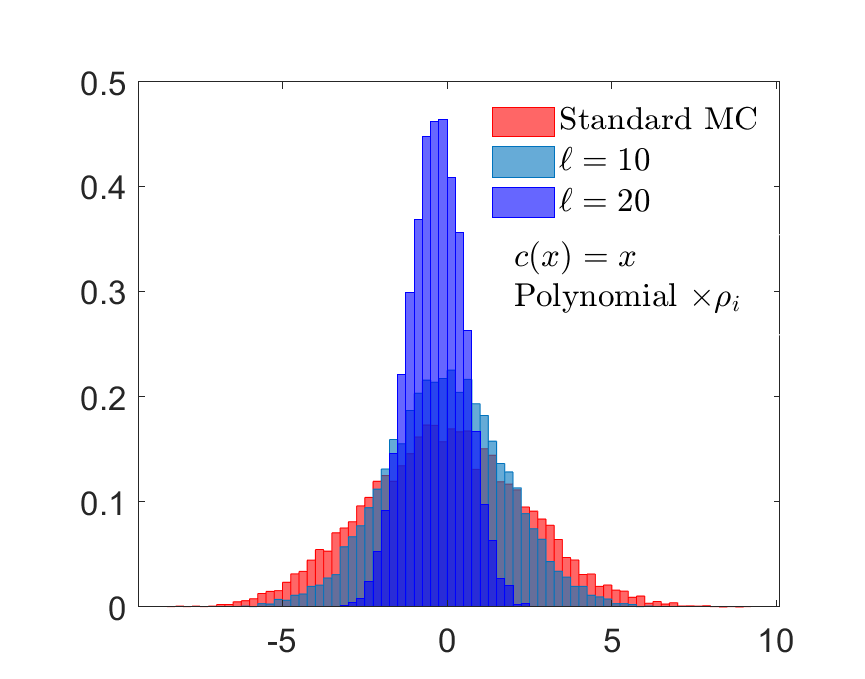
\includegraphics[width=0.5\hsize]{Chap5_hist_all_ds_basis_10000runs_100000samples.eps}}
	\subfloat {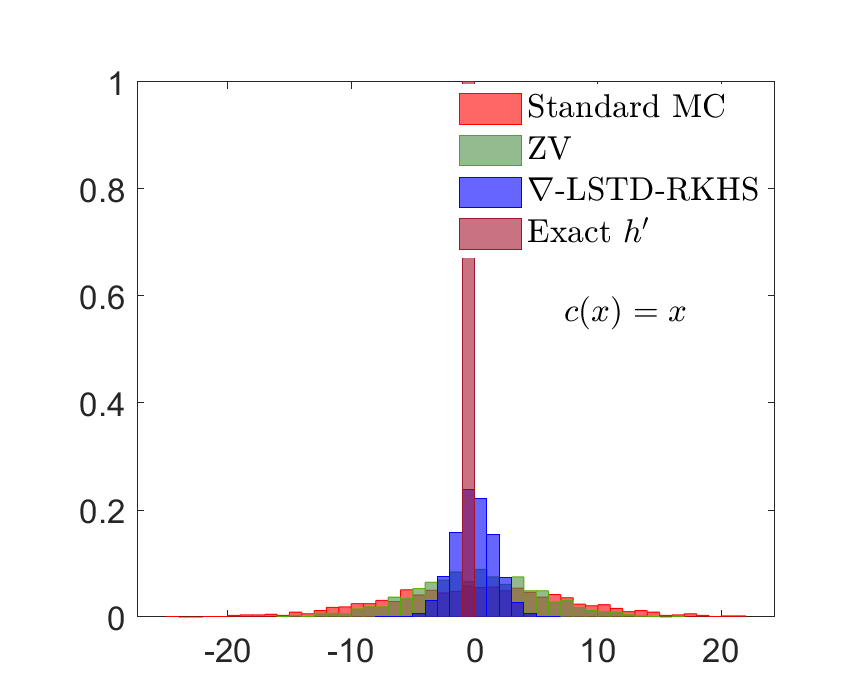
\includegraphics[width=0.5\hsize]{Chap5_hist_asym_var_all_methods.eps}}
}
\end{figure}
\end{frame}

\begin{frame}
\frametitle{Applications to MCMC}
\framesubtitle{Numerical Examples - RWM}
\begin{tabular}{lll}\alertb{Example:}   & Random walk Metropolis (RWM)
	\\
\end{tabular}
\begin{figure}
\centering
 \mbox{
	\subfloat{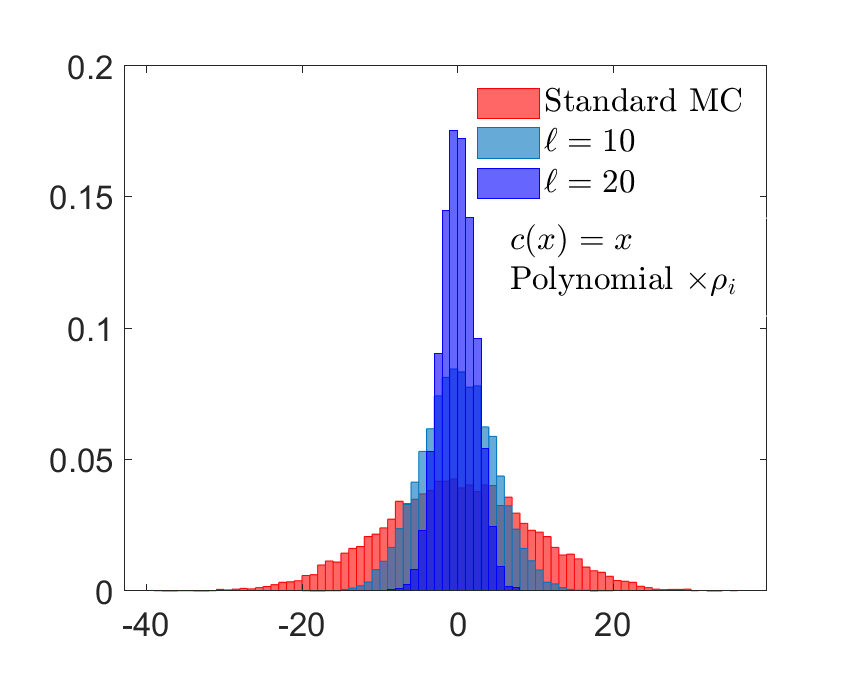
\includegraphics[width = 0.5\hsize]{Chap5_hist_mh_all_ds_basis_10000runs_100000samples.eps}} 
	\subfloat{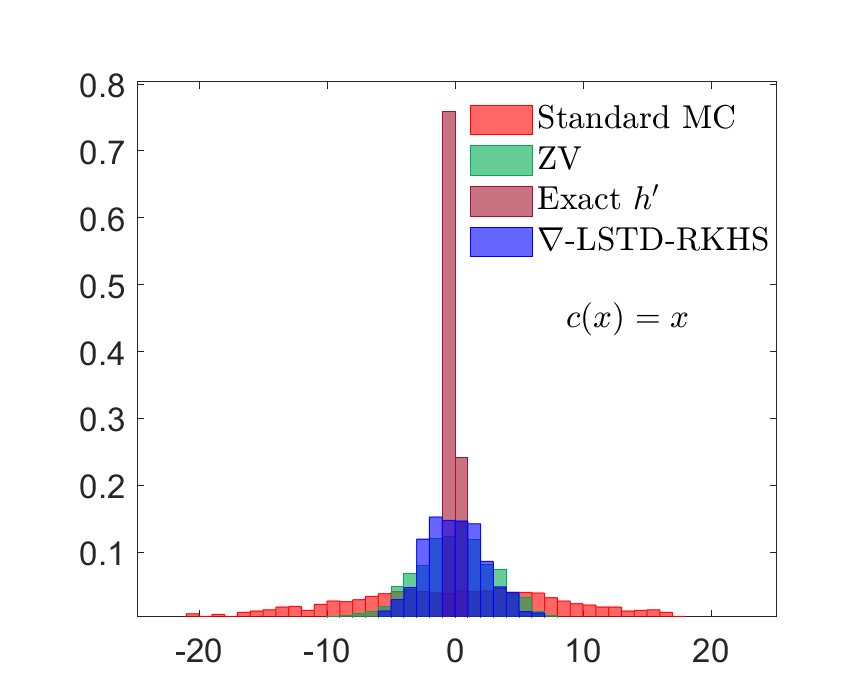
\includegraphics[width=0.5\hsize]{Chap5_hist_mh_asym_var_all_methods.eps}}
} 
\end{figure}
\end{frame}


\begin{frame}
\frametitle{Applications to MCMC}
\framesubtitle{Numerical Examples - ULA v RWM}
Unadjusted Langevin algorithm (ULA) vs Random walk Metropolis (RWM) \\[-0.2cm]
\begin{figure}[h]
	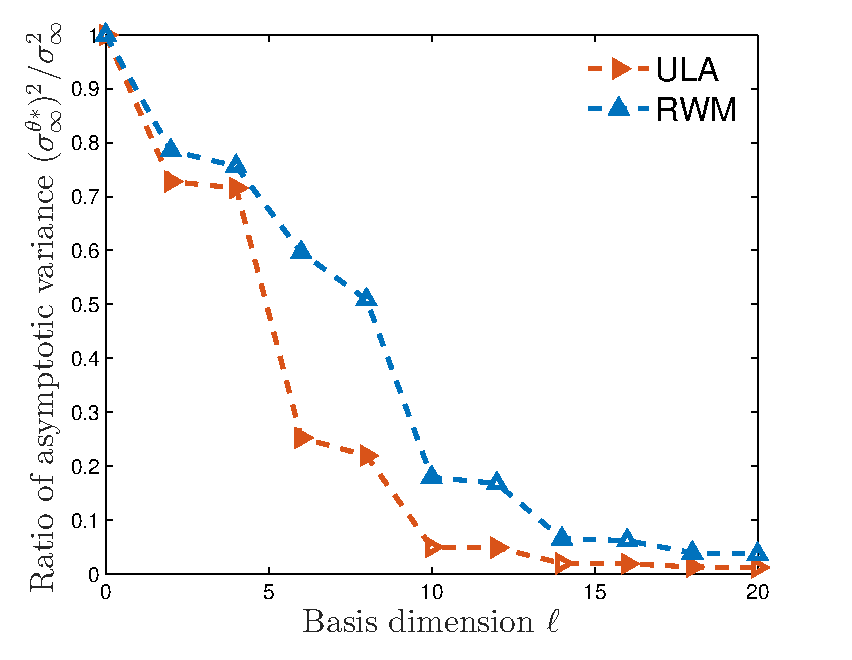
\includegraphics[width = .6\hsize]{Chap5_rel_red_lang_mh_all.eps}
	\label{lang_mh}
\end{figure}
\end{frame}

\begin{frame}
\frametitle{Applications to MCMC}
\framesubtitle{Numerical Examples - Sample variance v Asymptotic variance}
Sample variance v Asymptotic variance
\[
\begin{aligned}
\sigma^2 &= \langle \tilc, \tilc\rangle_{L^2} = R(0) \quad &\text{- Sample variance}\\ \pause
\gamma^2 & = 2 \langle h, \tilc \rangle_{L^2}   = \int_{-\infty}^{\infty} R(s) ds \quad &\text{- Asymptotic variance} \\ \pause
\end{aligned}
\]
Minimizing $\sigma^2$ is easier than minimizing $\gamma^2$  {\footnotesize \bl{[Oates 14,  Papamarkou 14] }}\\[0.2cm]
Appropriate only if samples are i.i.d. \\[0.2cm]
\alertb{Minimizing $\sigma^2$ also minimizes $\gamma^2$ ?} \pause \rd{NO !}
\end{frame}

\begin{frame}
\frametitle{Applications to MCMC}
\framesubtitle{Numerical Examples - Sample variance vs Asymptotic variance}
\begin{tabular}{lll}\alertb{Example:}   & Unadjusted Langevin algorithm (ULA)
	\\ & $c(x) \equiv x$ 
\end{tabular}
\begin{figure}
	\centering
	\mbox{
	\subfloat{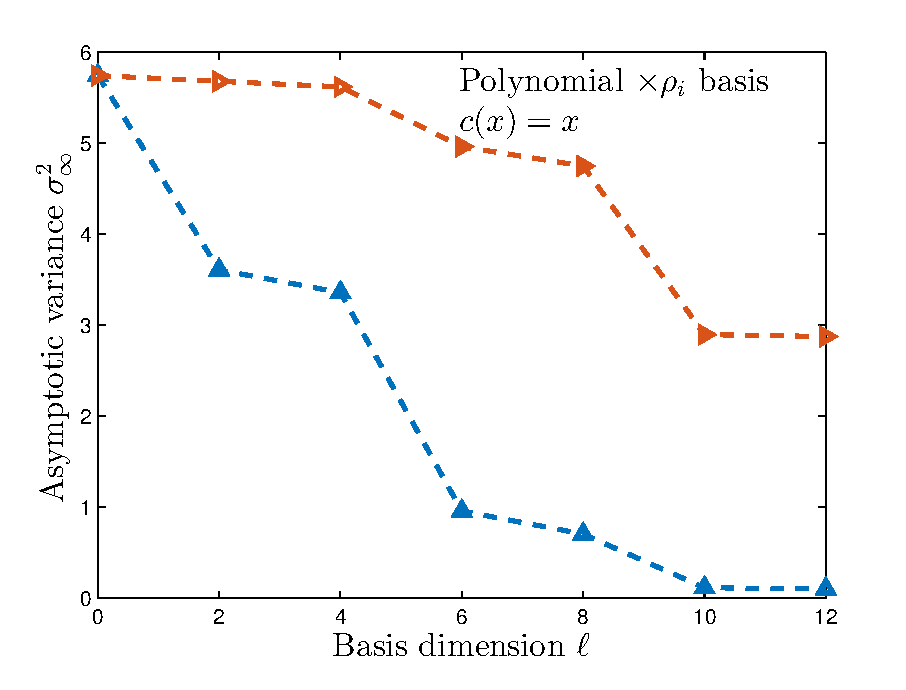
\includegraphics[width = .48\hsize]{Chap5_x_var_vs_asym_var_wt_poly.eps}}
	\subfloat{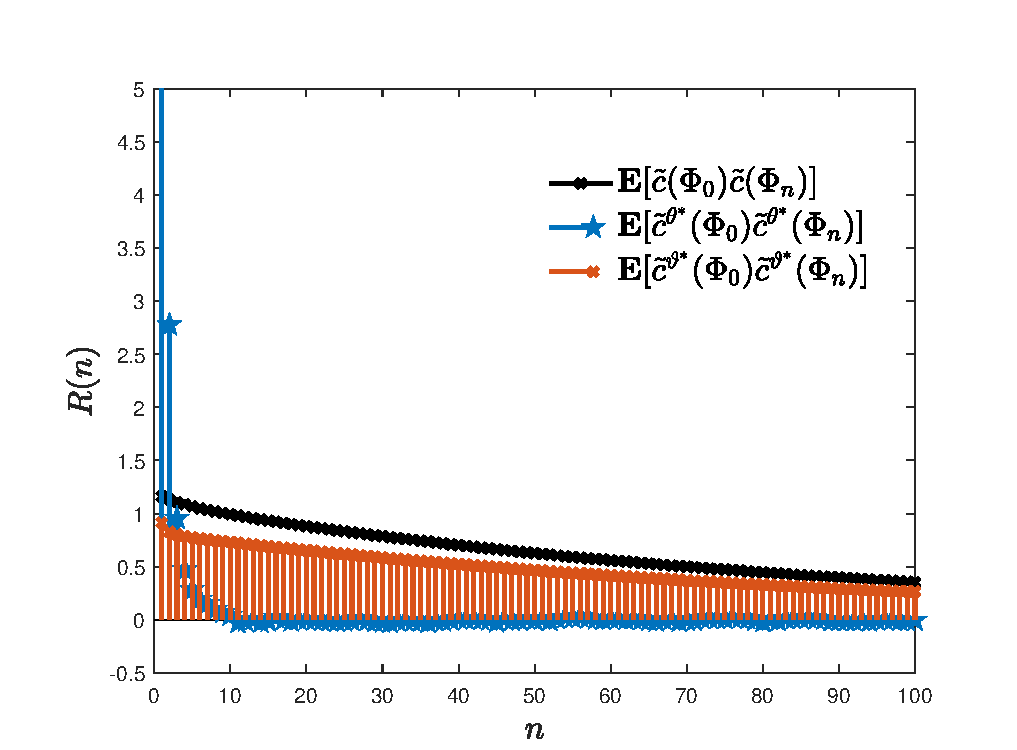
\includegraphics[width = .52\hsize]{Chap5_cov_R_n_gamma_pt05.eps}}
}
\end{figure}
\end{frame}

\begin{frame}
\frametitle{Applications to MCMC}
\framesubtitle{Numerical Examples - Logistic regression with RWM sampling}
\begin{tabular}{lll}\alertb{Example:}   & Logistic Regression for Swiss bank notes
	\\
\end{tabular}\\[0.3cm]
$X \in \Re^{200 \times 4}$ - Covariates measurements of four features of $200$ bank notes. \\[0.1cm]
$\{Y_i  \in \{0,1\}, 1 \leq i \leq 200 \}$ -  Binary response variables. \\[0.1cm]
$\Theta \in \Re^4$ - Regression coefficients for classification.
\[
\begin{aligned}
\pr(\Theta| \{X_i,Y_i\}_1^N) & \propto \\ \exp & \left( \underbrace{\sum_{i=1}^N \{Y_i \Theta^\transpose X_i - \log(1+e^{\Theta^\transpose X_i} ) \}}_{\text{Likelihood}} - \underbrace{\frac{\Theta^\transpose \Sigma^{-1} \Theta}{2}}_{\text{Prior}} \right)
\end{aligned}
\]
\end{frame}

\begin{frame}
\frametitle{Applications to MCMC}
\framesubtitle{Numerical Examples - Logistic Regression with RWM sampling}
\begin{tabular}{lll}\alertb{Example:}   & Logistic Regression for Swiss bank notes
	\\
\end{tabular}
\begin{figure}
\centering
\mbox{
	\subfloat{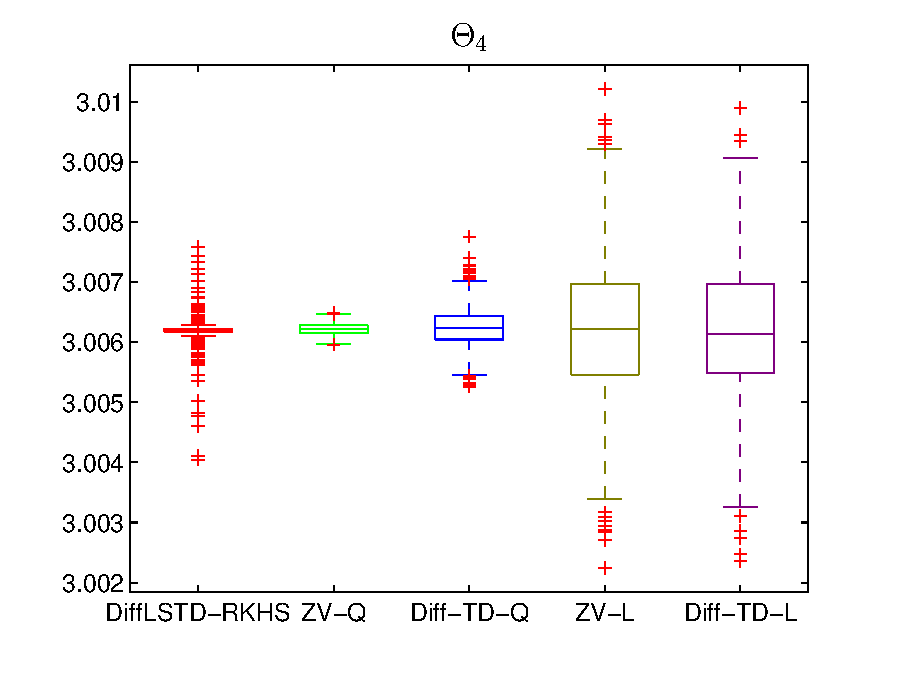
\includegraphics[width=0.5\hsize]{Chap5_hist_Theta4_no_std.eps}}
	\subfloat{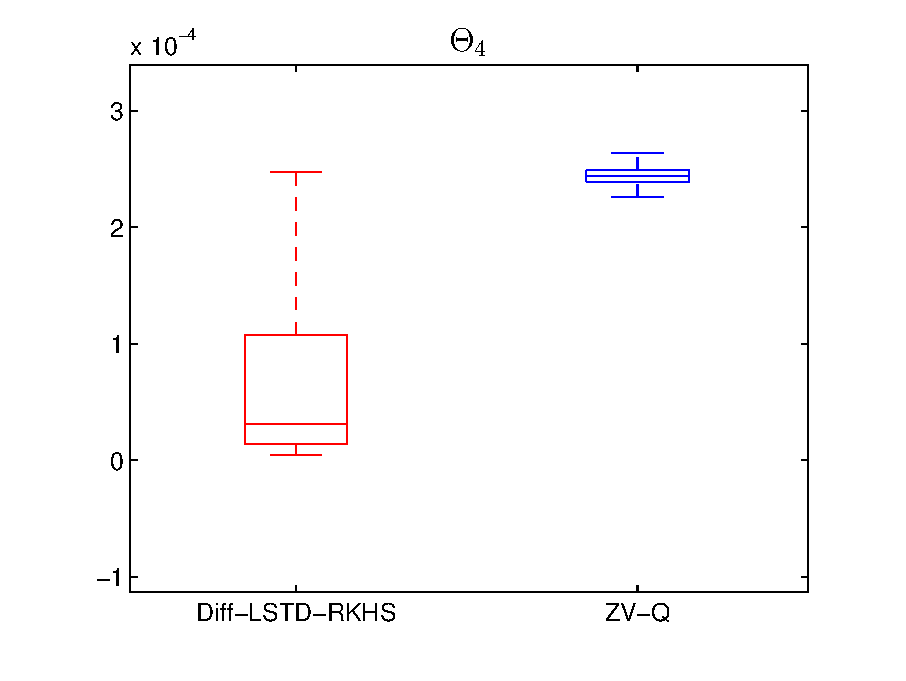
\includegraphics[width=0.5\hsize]{Chap5_box_var_Theta4.eps}}
}
	Box plots of estimates of $\Theta_4$.
\end{figure}
\end{frame}

\section{Conclusions and Future Work}
\begin{frame}
\frametitle{Conclusions}
\begin{itemize}
	\item Differential LSTD learning based approaches to approximate solution to Poisson's equation for the Langevin diffusion.\\[-0.1cm]
	 \begin{itemize}
	 	\item Finite dimensional basis.
	 	\item RKHS.
	 \end{itemize}
	\item Two interesting applications
	\begin{itemize}
		\item Asymptotic variance reduction in MCMC algorithms.
		\item Gain function approximation in Feedback particle filter.
	\end{itemize}
	\item Extended the approach to include reversible Markov chains.
\end{itemize}
\end{frame}

%\begin{frame}
%\frametitle{Future Work}
%\begin{itemize}
%	\item[$\bullet$]
%	Create algorithms whose complexity does not grow with dimension.
%	\item[$\bullet$]
%	A tractable solution to the ERM with regularized gradient may also lead to more efficient algorithms.
%	
%	\item[$\bullet$] Solidarity with the prior work  will require the extension of the RKHS theory to the case of self-adjoint kernels that are not symmetric.
%	
%	\item[$\bullet$]
%	Research and large scale testing is required for nonlinear filtering and MCMC applications.
%	
%\end{itemize}
%\end{frame}

\begin{frame}
\frametitle{References}
\bibliographystyle{alpha}
\begin{thebibliography}{10}
	\tiny
	\bibitem{raddevmey16}
	A. Radhakrishnan, A. Devraj and S. Meyn, ``Learning techniques for feedback particle filter design,'' \textit{ 2016 IEEE 55th Conference on Decision and Control (CDC)}, Las Vegas, NV, 2016.
	\bibitem{radmey18}
	A. Radhakrishnan, S. Meyn, ``Feedback particle filter design using a differential-loss reproducing kernel Hilbert space,'' \textit{2018 American Control Conference (ACC)}, Milwaukee, WI, 2018.
	\bibitem{ctcn}
	S.P.Meyn, ``Control Techniques for Complex Networks'', \textit{Cambridge University Press}, Dec 2007.
	\bibitem{henderson}
	S. Henderson. \textit{Variance Reduction Via an Approximating Markov Process}. PhD thesis, Stanford University, Stanford, California, 1997.
	\bibitem{yang}
	T. Yang, P. G. Mehta and S. P. Meyn, ``Feedback Particle Filter,'' in IEEE Transactions on Automatic Control, vol. 58, no. 10, pp. 2465-2480, Oct. 2013.
	
	\bibitem{devraj}
	A. M. Devraj and S. P. Meyn, ``Differential LSTD learning for value function approximation,'' \textit{2016 IEEE 55th Conference on Decision and Control (CDC)}, Las Vegas, NV, 2016.
	
	\bibitem{zhou}
	D.X. Zhou,
``Derivative reproducing properties for kernel methods in learning theory,''\textit{Journal of Computational and Applied Mathematics},
 Vol. 220, Issues 1?2,
	2008.
	
\end{thebibliography}
\end{frame}



\begin{frame}
% \centerline{\includegraphics[width=.9\hsize]{DSC04173.jpg}}
\centerline{\bf \huge \color{OrangeRed} Thank You!}
\vfill
\centerline{\huge \alertb{Questions?}}
\vfill
\end{frame}



\end{document}
%----------------------------------------------------------------------------------------------------------------------





% \centerline{\includegraphics[width=.9\hsize]{DSC04173.jpg}}
\centerline{\bf \huge \color{OrangeRed} Thank You!}
\vfill

\end{frame}

\begin{frame}
	\frametitle{References}
	\bibliographystyle{alpha}
	\begin{thebibliography}{10}
	\small
		\bibitem{asmglynn}
		S. Asmussen and P. W. Glynn. Stochastic Simulation: Algorithms and Analysis, volume 57 of \textit{Stochastic Modelling and Applied Probability.} Springer-Verlag, New York, 2007.
		
		\bibitem{glynnmeyn}
		P. W. Glynn and S. P. Meyn, A Liapunov bound for solutions of the Poisson equation, 1996.
		
		\bibitem{henderson}
		S. Henderson. \textit{Variance Reduction Via an Approximating Markov Process}. PhD thesis, Stanford University, Stanford, California, 1997.
		
		\bibitem{hendersonmeyn}
		S. G. Henderson, S. P. Meyn, and V. B. Tadic. Performance evaluation and policy selection in multiclass networks, 2003
		
		\bibitem{ctcn}
		S.P.Meyn, `Control Techniques for Complex Networks', \textit{Cambridge University Press}, Dec 2007
		
	\end{thebibliography}
\end{frame}
\end{document}

\bibliographystyle{abbrv}
\bibliography{markov,q} 